\documentclass[a4paper,12pt]{article}
\usepackage[colorlinks=false,pdfborder=000]{hyperref}
\usepackage[top=1.2in, bottom=1.2in, left=1.2in, right=1.2in]{geometry}
\usepackage[dvips]{graphicx,color}
\usepackage{times}
\usepackage{tikz}
\usepackage{fp}
\usetikzlibrary {snakes,arrows}

%%%%%%%%%%%%%%%%%%%%%%%%%%%%%%%%%%%%%%%%%%%%%%%%%%%%%%%%%%%%%%%%%%
\def\scale{0.7}
\def\half{0.5}
\providecommand{\blockage}[4]{%
    \fill[block] (#1,#2) rectangle (#3+1,#4+1);
}
\providecommand{\drawrowcol}[2]{
    % enumerate the row and column
    \FPset{\row}{#1}
    \FPadd{\row}{\row}{-1}
    \foreach \r in {0,...,\row}
        \node at (0-\half,\r+\half) {\r} ;
    \FPset{\col}{#2}
    \FPadd{\col}{\col}{-1}
    \foreach \c in {0,...,\col}
        \node at (\c+\half,0-\half) {\c} ;
}
\providecommand{\drawgrid}[2]{
    \draw (0,0) grid (#1,#2);
    \drawrowcol{#1}{#2}
}
\providecommand{\drawtwopin}[7]{
%#1= pin1 name #2,#3=pin1 location
%#4= pin1 name #5,#6=pin2 location
%#7= color
    \node[pins,#7]  (#1) at (#2 + \half, #3 + \half) {}; % pin-1
    \node[pins,#7]  (#4) at (#5  + \half, #6 + \half) {}  % pin-2
        edge[arrow] (#1);            % arrow
    %\node[above] at (#1) {$#1$}; % label
    %\node[above] at (#4) {$#4$}; % label
}
\providecommand{\drawthreepin}[9]{
%#1= pin1 name #2,#3=pin1 location
%#4= pin1 name #5,#6=pin2 location
%#7= pin1 name #8,#9=pin3 location
    \node[pins]  (#1) at (#2 + \half, #3 + \half) {}; % pin-1
    \node[pins]  (#4) at (#5  + \half, #6 + \half) {}  % pin-2
        edge[arrow] (#1);            % arrow
    \node[pins]  (#7) at (#8  + \half, #9 + \half) {}  % pin-2
        edge[arrow] (#1);            % arrow
}
%%%%%%%%%%%%%%%%%%%%%%%%%%%%%%%%%%%%%%%%%%%%%%%%%%%%%%%%%%%%%%%%%%
\begin{document}

\begin{figure}
\centering
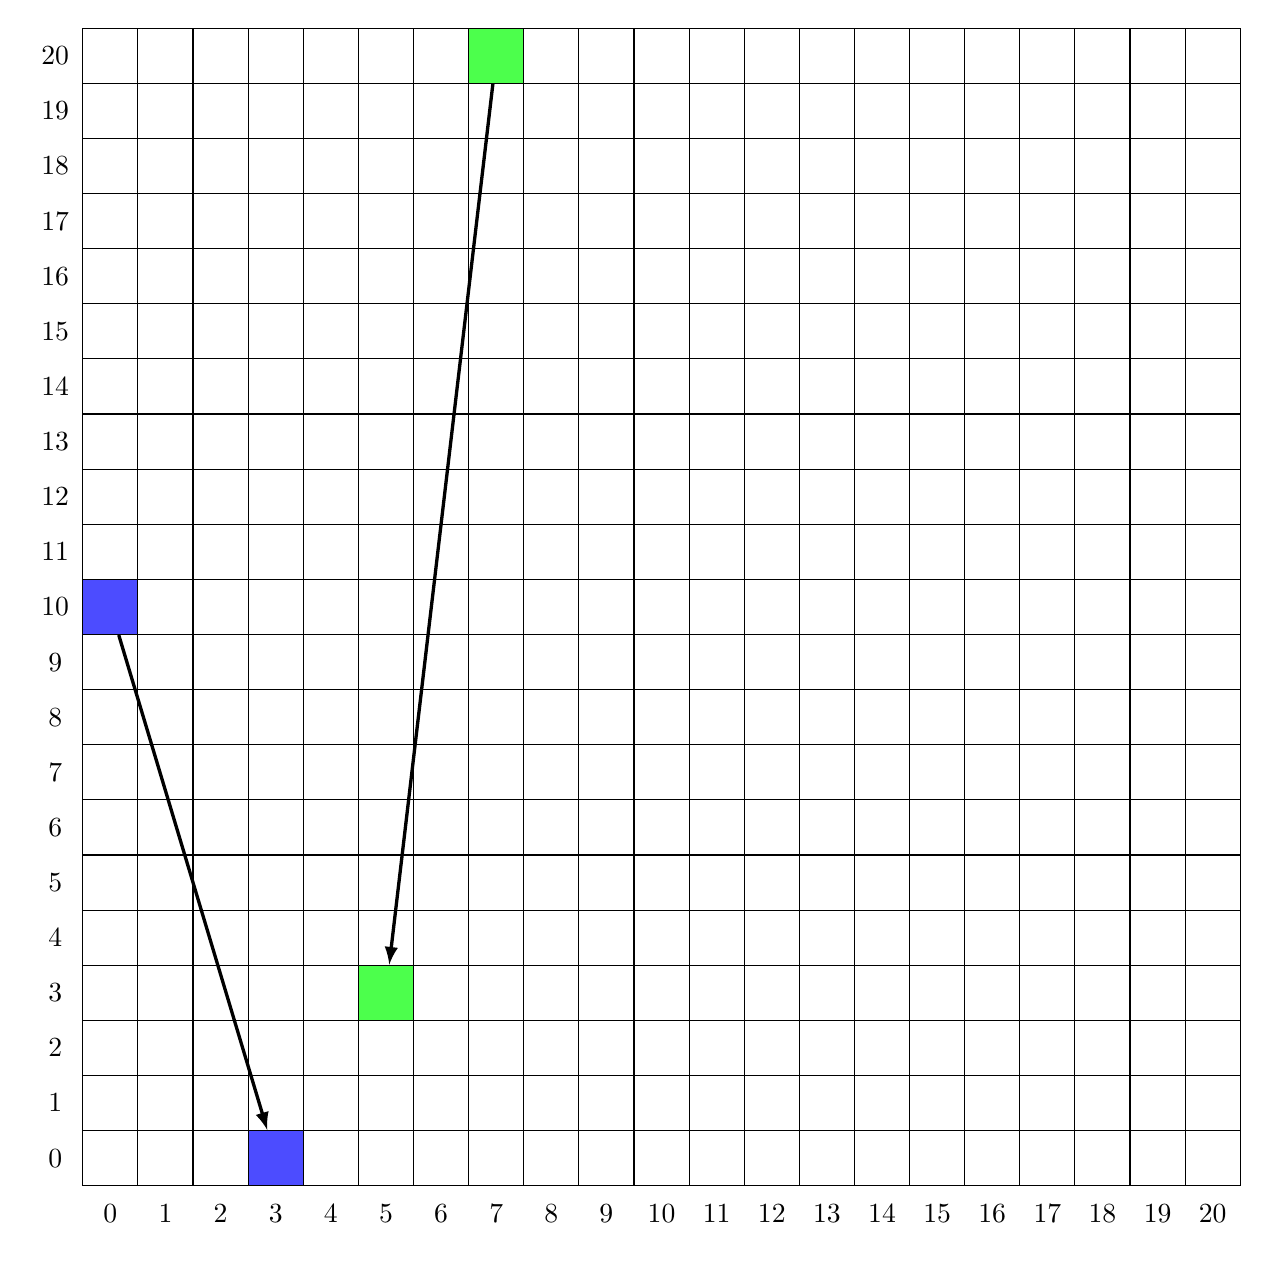
\begin{tikzpicture}[scale=\scale,
	%inner sep=1cm*\scale*\half,
	inner sep=0,
	minimum size=1cm*\scale,
	>=latex,
	pins/.style={rectangle,draw,fill=brown,font=\scriptsize},
	arrow/.style={->,very thick},
	block/.style={gray}]
	% define the row and column number
	\def \N{21}\def \M{21}
	% blockages
	% nets
	\drawtwopin{Dlt01}{3}{0}{Sample}{0}{10}{blue!70}
	\drawtwopin{Dlt01}{5}{3}{B1}{7}{20}{green!70}
	\drawgrid{\N}{\M}
	\end{tikzpicture}
	\caption{DAC05\_subproblem\_1}
	\end{figure}
	\clearpage
	\begin{figure}
	\centering
	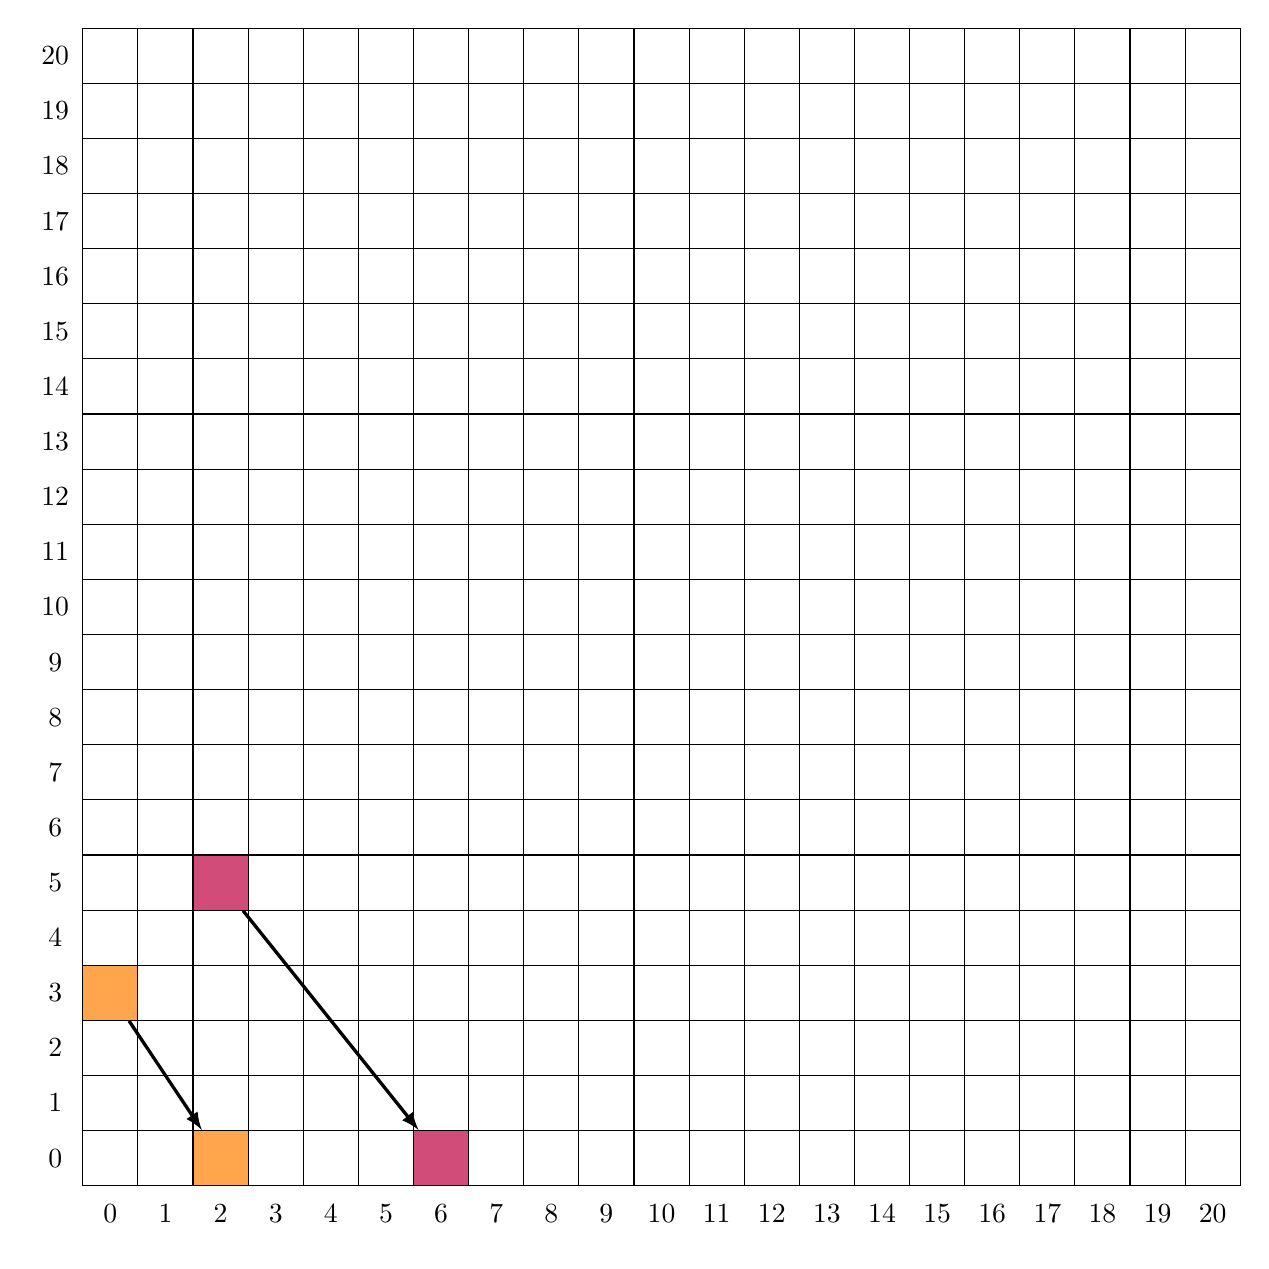
\begin{tikzpicture}[scale=\scale,
	%inner sep=1cm*\scale*\half,
	inner sep=0,
	minimum size=1cm*\scale,
	>=latex,
	pins/.style={rectangle,draw,fill=brown,font=\scriptsize},
	arrow/.style={->,very thick},
	block/.style={gray}]
	% define the row and column number
	\def \N{21}\def \M{21}
	% blockages
	% nets
	\drawtwopin{Dlt01_to_Dlt02}{2}{0}{Dlt01}{0}{3}{orange!70}
	\drawtwopin{Dlt01_to_Dlt03}{6}{0}{Dlt01}{2}{5}{purple!70}
	\drawgrid{\N}{\M}
	\end{tikzpicture}
	\caption{DAC05\_subproblem\_2}
	\end{figure}
	\clearpage
	\begin{figure}
	\centering
	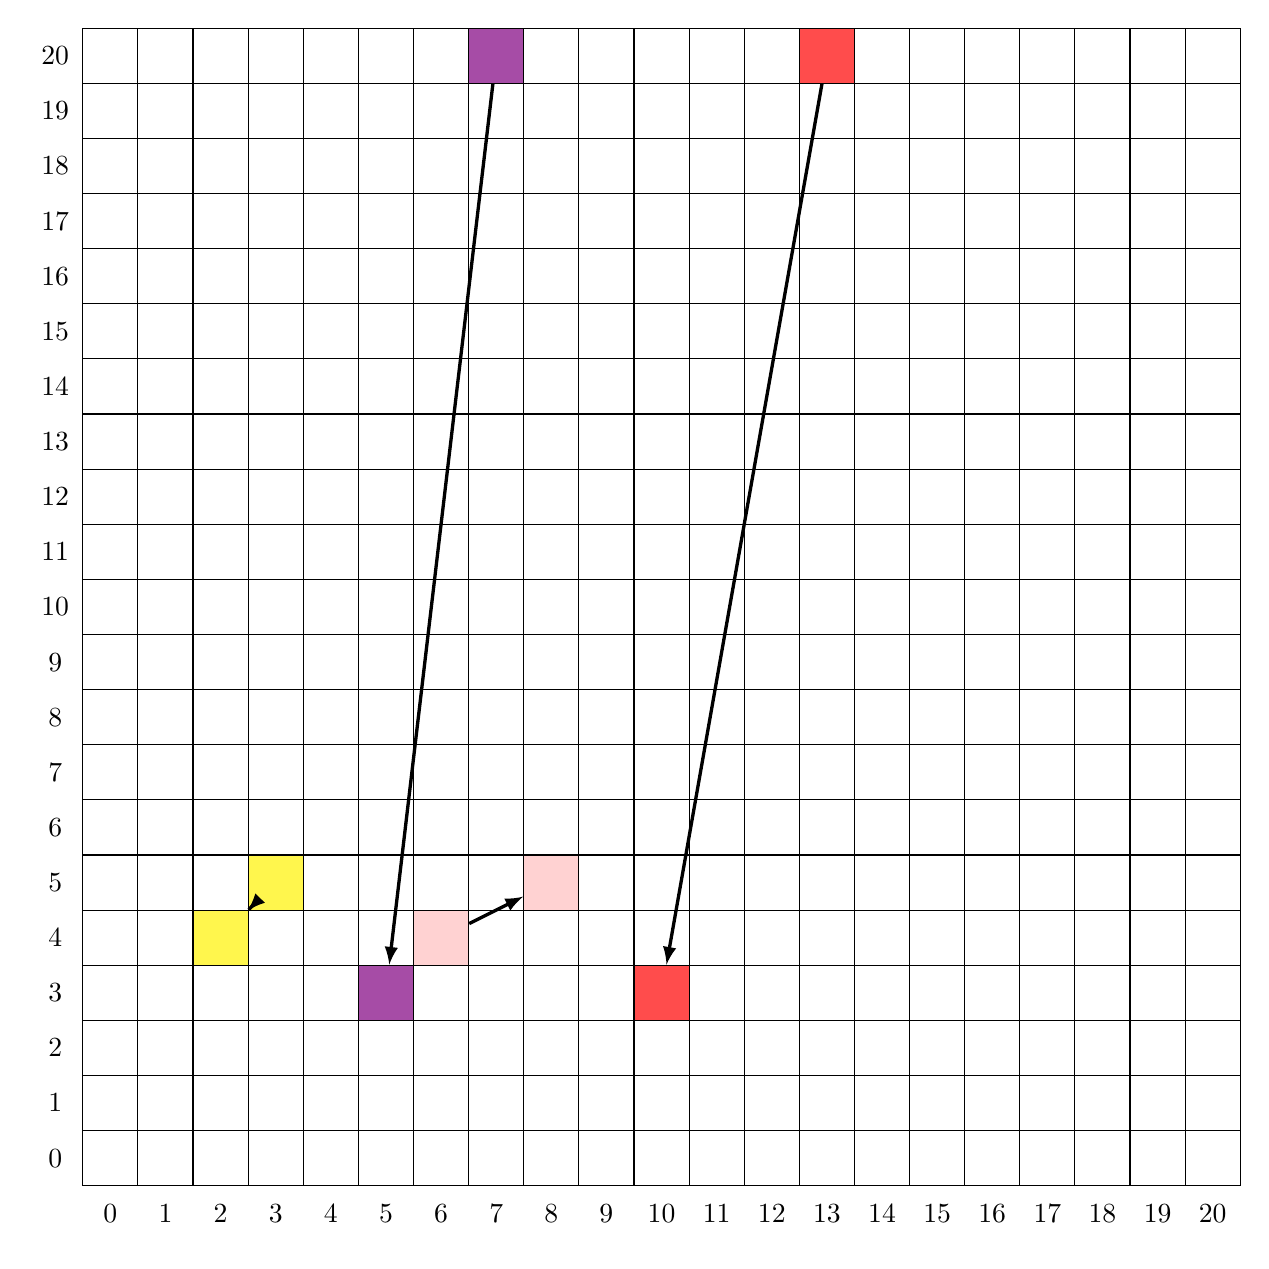
\begin{tikzpicture}[scale=\scale,
	%inner sep=1cm*\scale*\half,
	inner sep=0,
	minimum size=1cm*\scale,
	>=latex,
	pins/.style={rectangle,draw,fill=brown,font=\scriptsize},
	arrow/.style={->,very thick},
	block/.style={gray}]
	% define the row and column number
	\def \N{21}\def \M{21}
	% blockages
	% nets
	\drawtwopin{Dlt02}{3}{5}{Dlt01_to_Dlt02}{2}{4}{yellow!70}
	\drawtwopin{Dlt03}{8}{5}{Dlt01_to_Dlt03}{6}{4}{pink!70}
	\drawtwopin{Dlt02}{5}{3}{B1}{7}{20}{violet!70}
	\drawtwopin{Dlt03}{10}{3}{B2}{13}{20}{red!70}
	\drawgrid{\N}{\M}
	\end{tikzpicture}
	\caption{DAC05\_subproblem\_3}
	\end{figure}
	\clearpage
	\begin{figure}
	\centering
	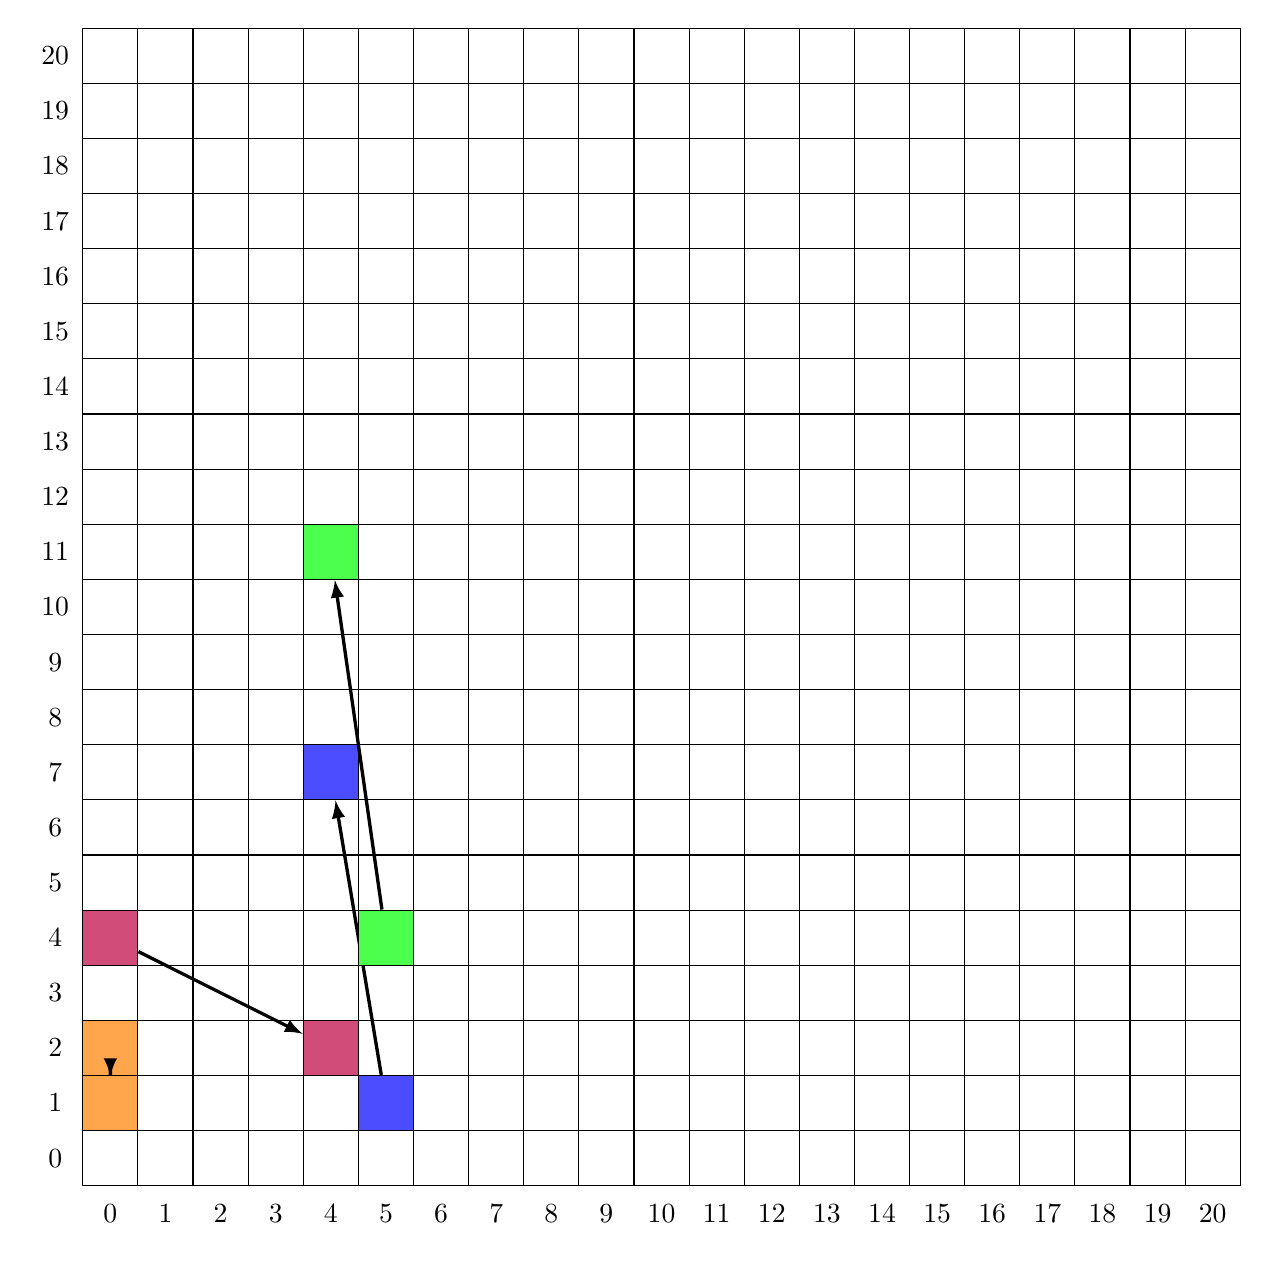
\begin{tikzpicture}[scale=\scale,
	%inner sep=1cm*\scale*\half,
	inner sep=0,
	minimum size=1cm*\scale,
	>=latex,
	pins/.style={rectangle,draw,fill=brown,font=\scriptsize},
	arrow/.style={->,very thick},
	block/.style={gray}]
	% define the row and column number
	\def \N{21}\def \M{21}
	% blockages
	% nets
	\drawtwopin{Dlt03_to_Dlt06}{4}{7}{Dlt03}{5}{1}{blue!70}
	\drawtwopin{Dlt03_to_Dlt07}{4}{11}{Dlt03}{5}{4}{green!70}
	\drawtwopin{Dlt02_to_Dlt04}{0}{2}{Dlt02}{0}{1}{orange!70}
	\drawtwopin{Dlt02_to_Dlt05}{4}{2}{Dlt02}{0}{4}{purple!70}
	\drawgrid{\N}{\M}
	\end{tikzpicture}
	\caption{DAC05\_subproblem\_4}
	\end{figure}
	\clearpage
	\begin{figure}
	\centering
	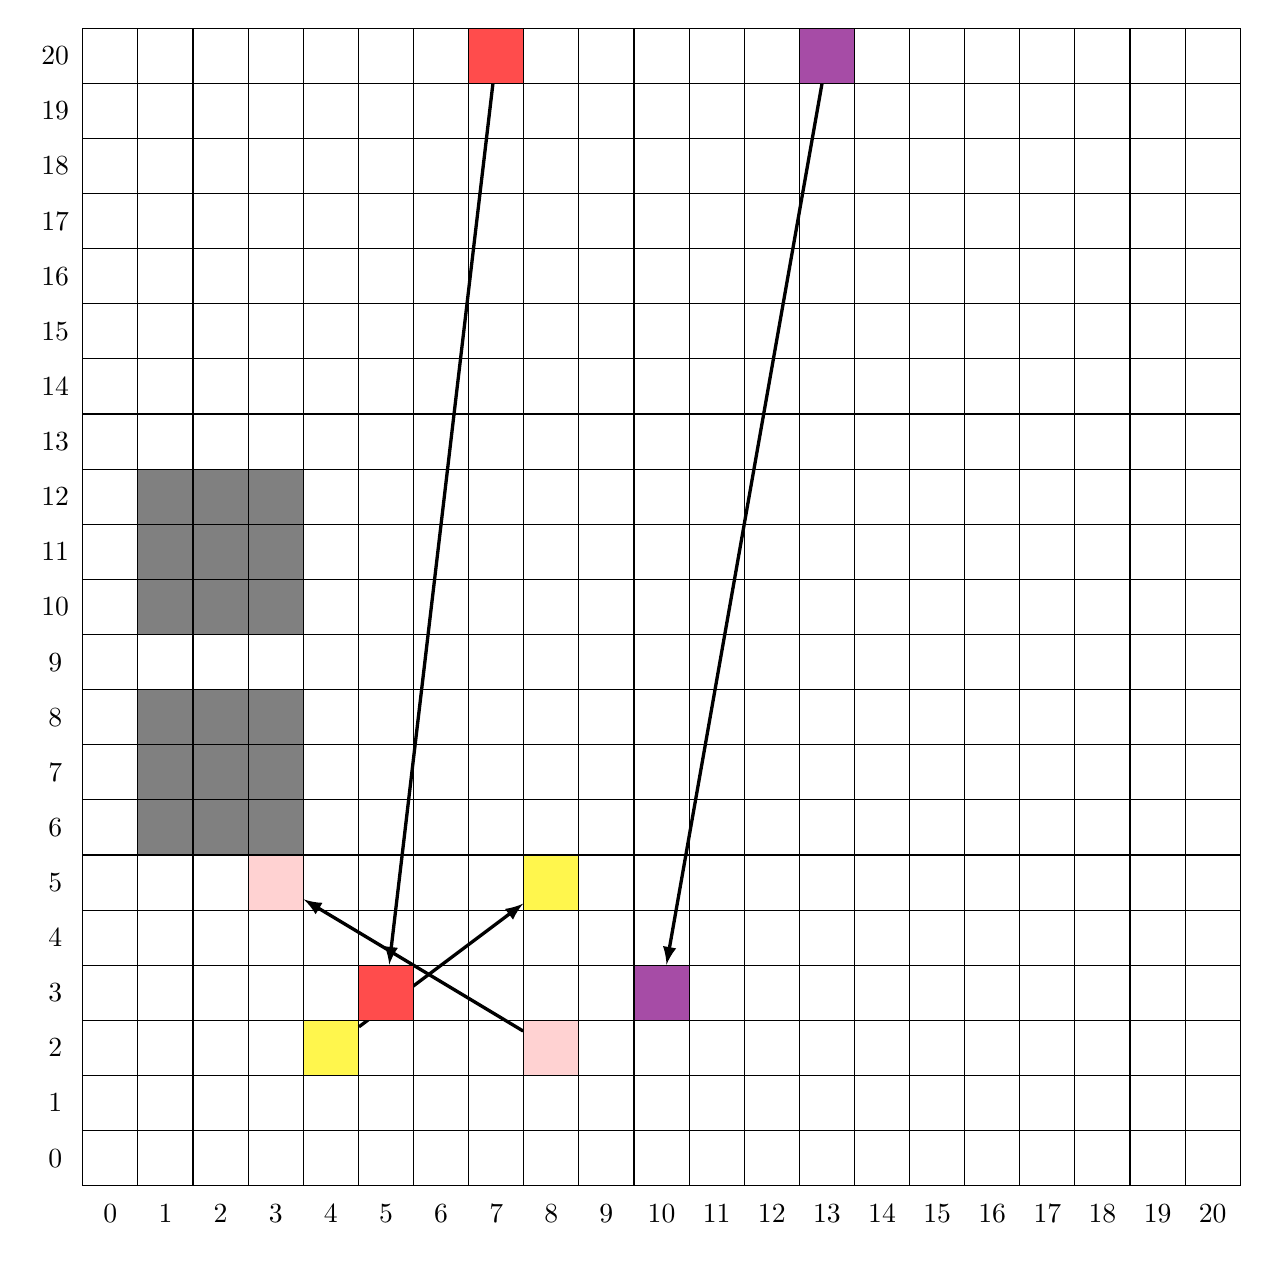
\begin{tikzpicture}[scale=\scale,
	%inner sep=1cm*\scale*\half,
	inner sep=0,
	minimum size=1cm*\scale,
	>=latex,
	pins/.style={rectangle,draw,fill=brown,font=\scriptsize},
	arrow/.style={->,very thick},
	block/.style={gray}]
	% define the row and column number
	\def \N{21}\def \M{21}
	% blockages
	\blockage{1}{6}{3}{8}
	\blockage{1}{10}{3}{12}
	% nets
	\drawtwopin{Dlt04}{8}{5}{Dlt02_to_Dlt04}{4}{2}{yellow!70}
	\drawtwopin{Dlt05}{3}{5}{Dlt02_to_Dlt05}{8}{2}{pink!70}
	\drawtwopin{Dlt04}{10}{3}{B2}{13}{20}{violet!70}
	\drawtwopin{Dlt05}{5}{3}{B1}{7}{20}{red!70}
	\drawgrid{\N}{\M}
	\end{tikzpicture}
	\caption{DAC05\_subproblem\_5}
	\end{figure}
	\clearpage
	\begin{figure}
	\centering
	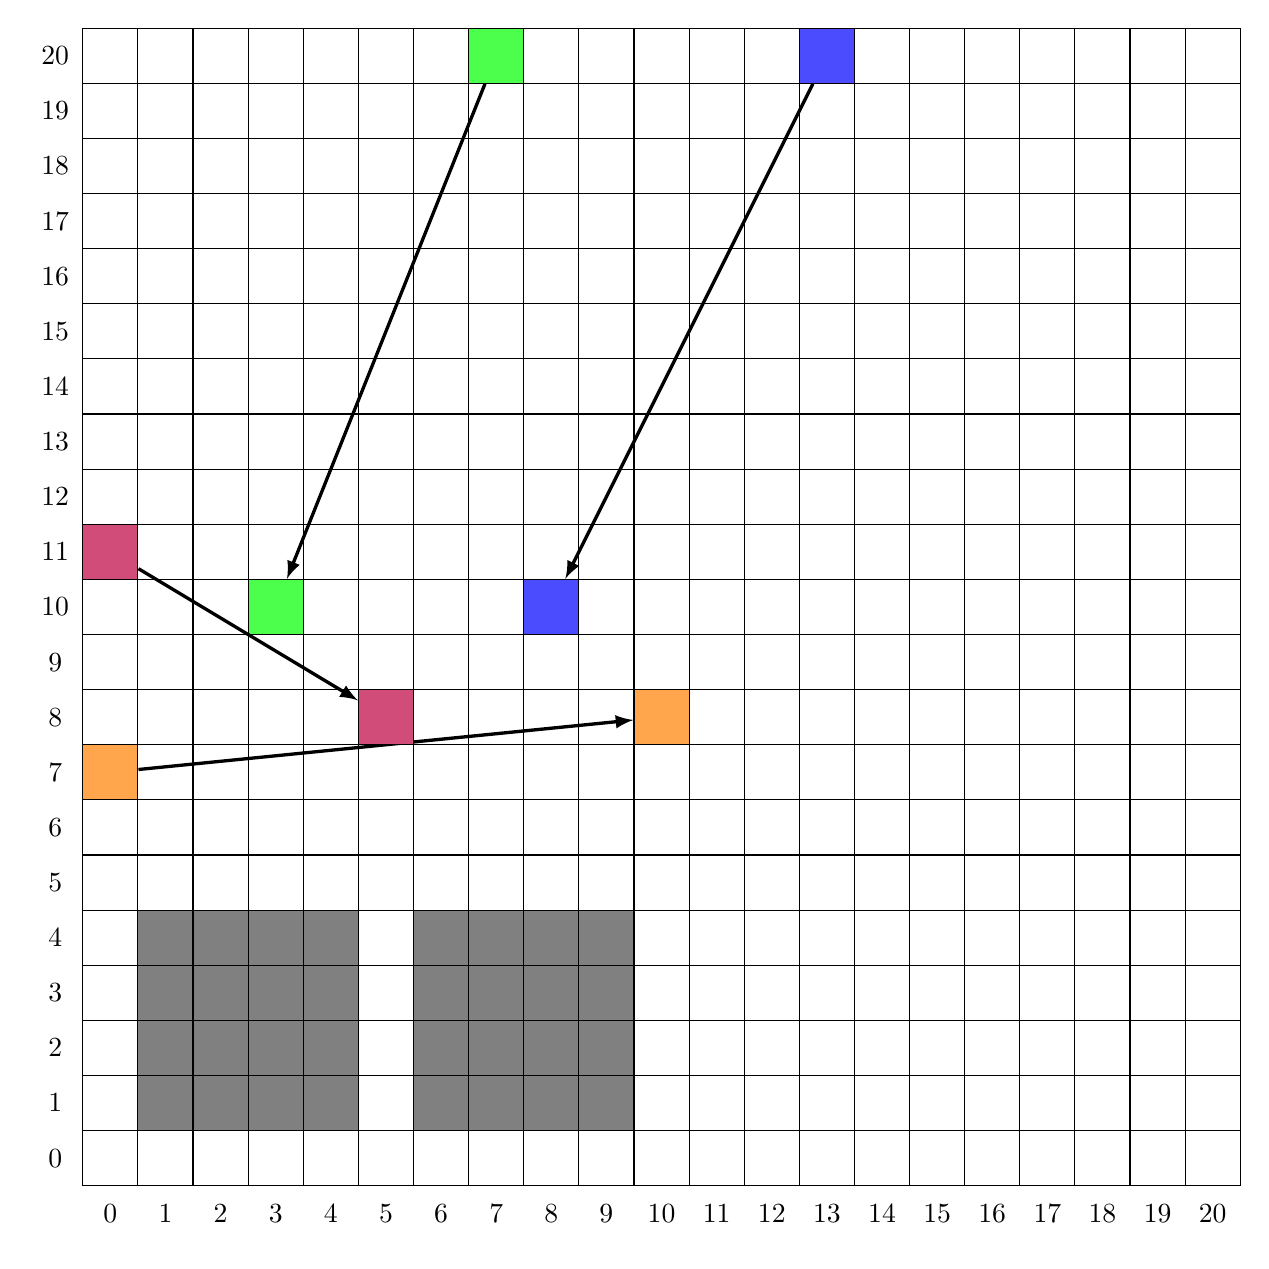
\begin{tikzpicture}[scale=\scale,
	%inner sep=1cm*\scale*\half,
	inner sep=0,
	minimum size=1cm*\scale,
	>=latex,
	pins/.style={rectangle,draw,fill=brown,font=\scriptsize},
	arrow/.style={->,very thick},
	block/.style={gray}]
	% define the row and column number
	\def \N{21}\def \M{21}
	% blockages
	\blockage{6}{1}{9}{4}
	\blockage{1}{1}{4}{4}
	% nets
	\drawtwopin{Dlt06}{8}{10}{B2}{13}{20}{blue!70}
	\drawtwopin{Dlt07}{3}{10}{B1}{7}{20}{green!70}
	\drawtwopin{Dlt06}{10}{8}{Dlt03_to_Dlt06}{0}{7}{orange!70}
	\drawtwopin{Dlt07}{5}{8}{Dlt03_to_Dlt07}{0}{11}{purple!70}
	\drawgrid{\N}{\M}
	\end{tikzpicture}
	\caption{DAC05\_subproblem\_6}
	\end{figure}
	\clearpage
	\begin{figure}
	\centering
	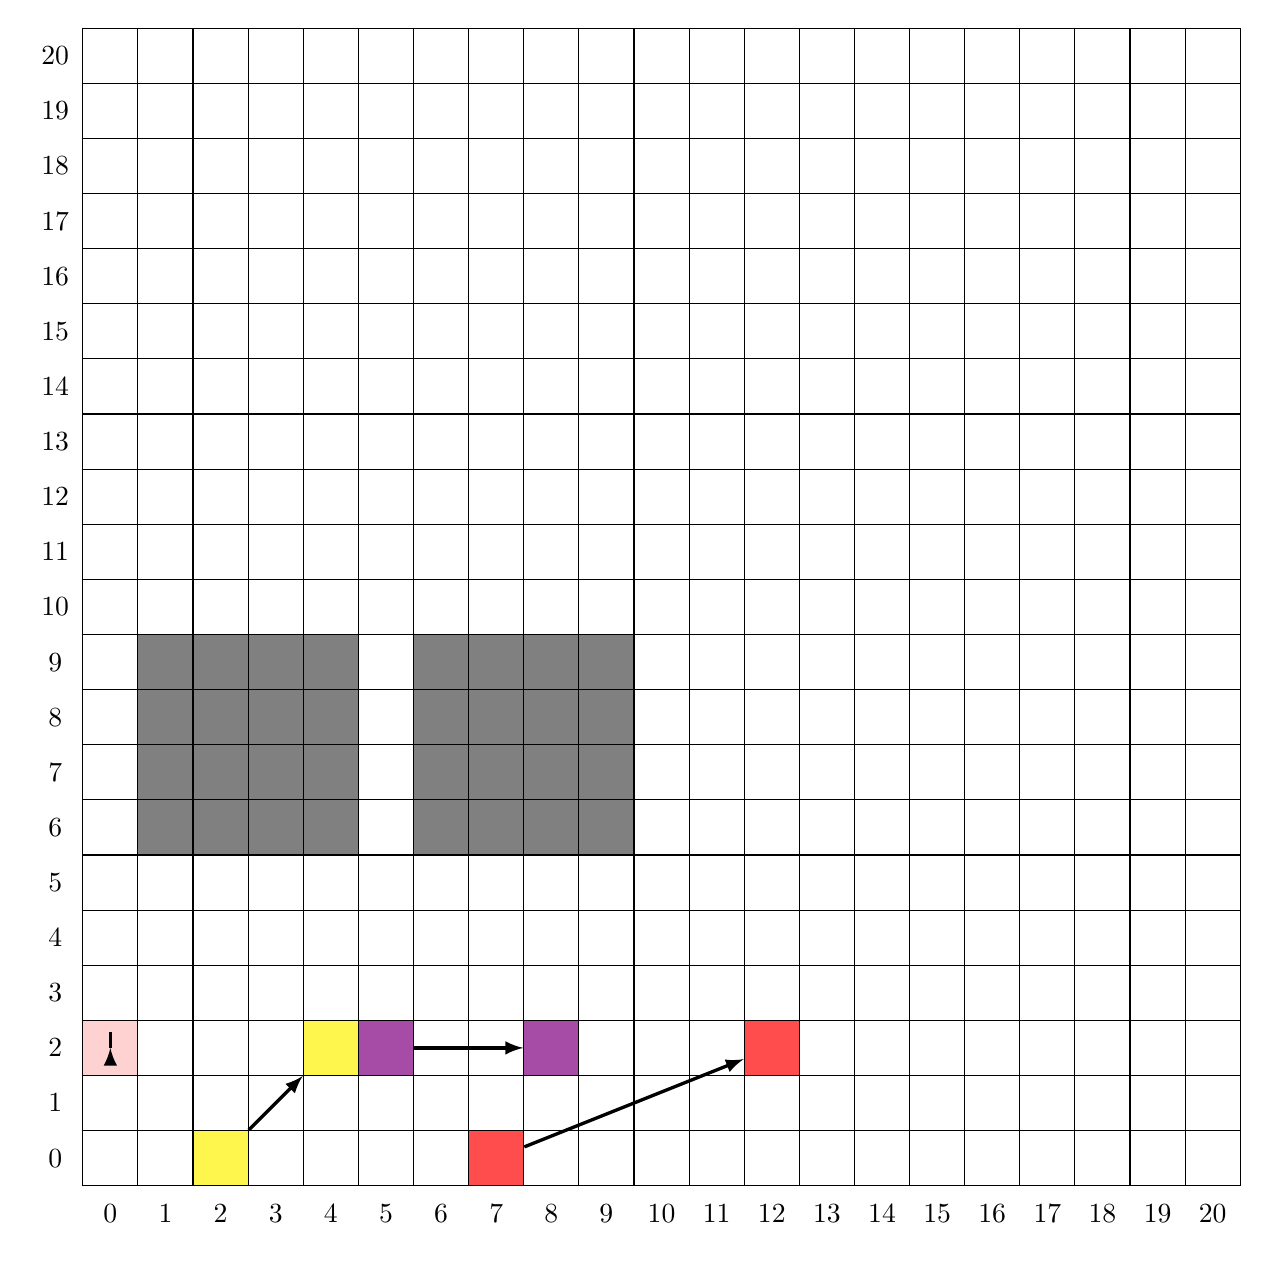
\begin{tikzpicture}[scale=\scale,
	%inner sep=1cm*\scale*\half,
	inner sep=0,
	minimum size=1cm*\scale,
	>=latex,
	pins/.style={rectangle,draw,fill=brown,font=\scriptsize},
	arrow/.style={->,very thick},
	block/.style={gray}]
	% define the row and column number
	\def \N{21}\def \M{21}
	% blockages
	\blockage{6}{6}{9}{9}
	\blockage{1}{6}{4}{9}
	% nets
	\drawtwopin{Dlt05_to_Dlt10}{4}{2}{Dlt05}{2}{0}{yellow!70}
	\drawtwopin{Dlt05_to_Dlt11}{0}{2}{Dlt05}{0}{2}{pink!70}
	\drawtwopin{Dlt04_to_Dlt08}{8}{2}{Dlt04}{5}{2}{violet!70}
	\drawtwopin{Dlt04_to_Dlt09}{12}{2}{Dlt04}{7}{0}{red!70}
	\drawgrid{\N}{\M}
	\end{tikzpicture}
	\caption{DAC05\_subproblem\_7}
	\end{figure}
	\clearpage
	\begin{figure}
	\centering
	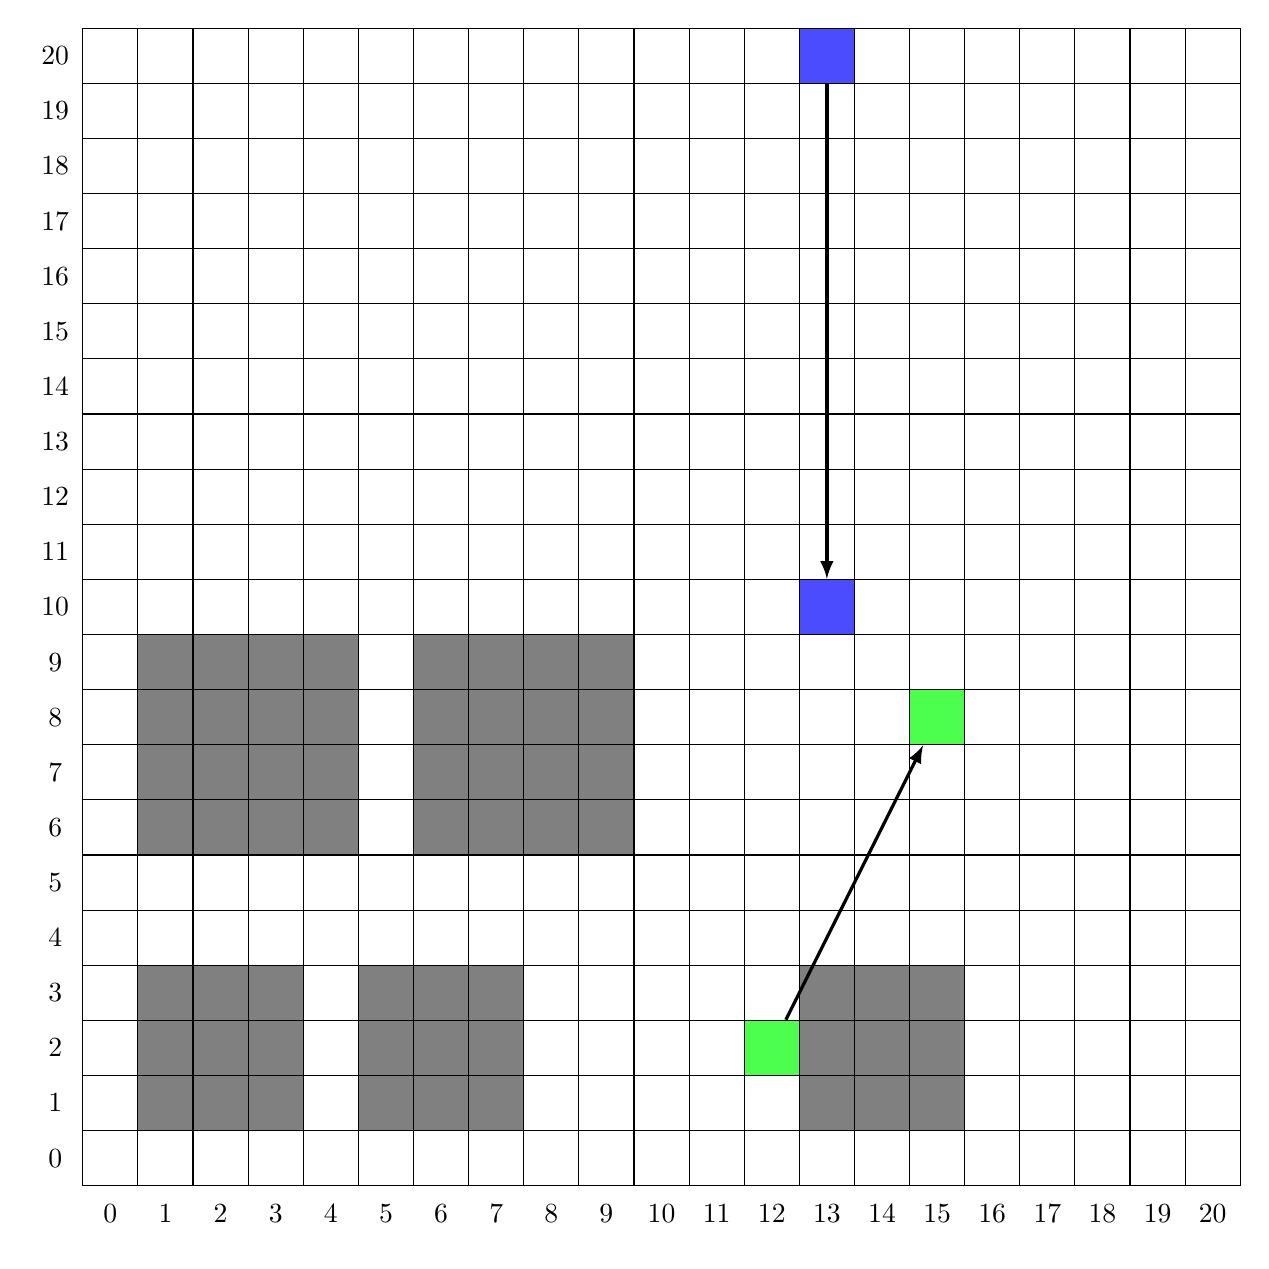
\begin{tikzpicture}[scale=\scale,
	%inner sep=1cm*\scale*\half,
	inner sep=0,
	minimum size=1cm*\scale,
	>=latex,
	pins/.style={rectangle,draw,fill=brown,font=\scriptsize},
	arrow/.style={->,very thick},
	block/.style={gray}]
	% define the row and column number
	\def \N{21}\def \M{21}
	% blockages
	\blockage{6}{6}{9}{9}
	\blockage{1}{6}{4}{9}
	\blockage{13}{1}{15}{3}
	\blockage{5}{1}{7}{3}
	\blockage{1}{1}{3}{3}
	% nets
	\drawtwopin{Dlt08}{13}{10}{B2}{13}{20}{blue!70}
	\drawtwopin{Dlt08}{15}{8}{Dlt04_to_Dlt08}{12}{2}{green!70}
	\drawgrid{\N}{\M}
	\end{tikzpicture}
	\caption{DAC05\_subproblem\_8}
	\end{figure}
	\clearpage
	\begin{figure}
	\centering
	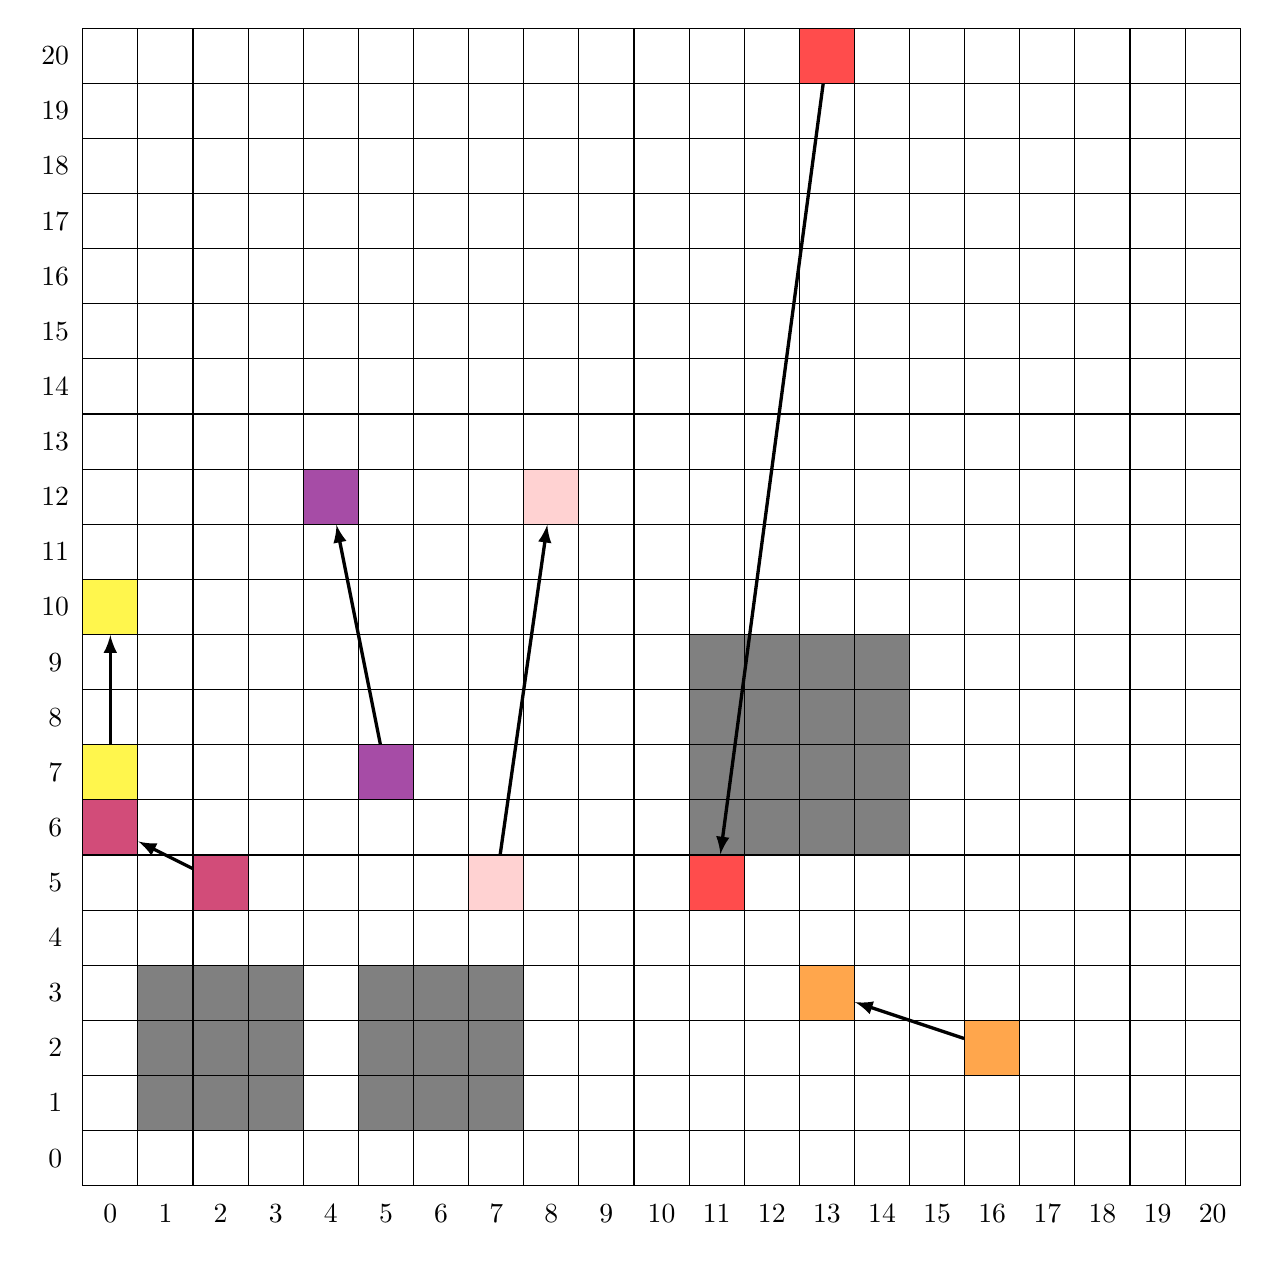
\begin{tikzpicture}[scale=\scale,
	%inner sep=1cm*\scale*\half,
	inner sep=0,
	minimum size=1cm*\scale,
	>=latex,
	pins/.style={rectangle,draw,fill=brown,font=\scriptsize},
	arrow/.style={->,very thick},
	block/.style={gray}]
	% define the row and column number
	\def \N{21}\def \M{21}
	% blockages
	\blockage{11}{6}{14}{9}
	\blockage{5}{1}{7}{3}
	\blockage{1}{1}{3}{3}
	% nets
	\drawtwopin{Dlt09}{13}{3}{Dlt04_to_Dlt09}{16}{2}{orange!70}
	\drawtwopin{Dlt07_to_Dlt14}{0}{6}{Dlt07}{2}{5}{purple!70}
	\drawtwopin{Dlt07_to_Dlt15}{0}{10}{Dlt07}{0}{7}{yellow!70}
	\drawtwopin{Dlt06_to_Dlt12}{8}{12}{Dlt06}{7}{5}{pink!70}
	\drawtwopin{Dlt06_to_Dlt13}{4}{12}{Dlt06}{5}{7}{violet!70}
	\drawtwopin{Dlt09}{11}{5}{B2}{13}{20}{red!70}
	\drawgrid{\N}{\M}
	\end{tikzpicture}
	\caption{DAC05\_subproblem\_9}
	\end{figure}
	\clearpage
	\begin{figure}
	\centering
	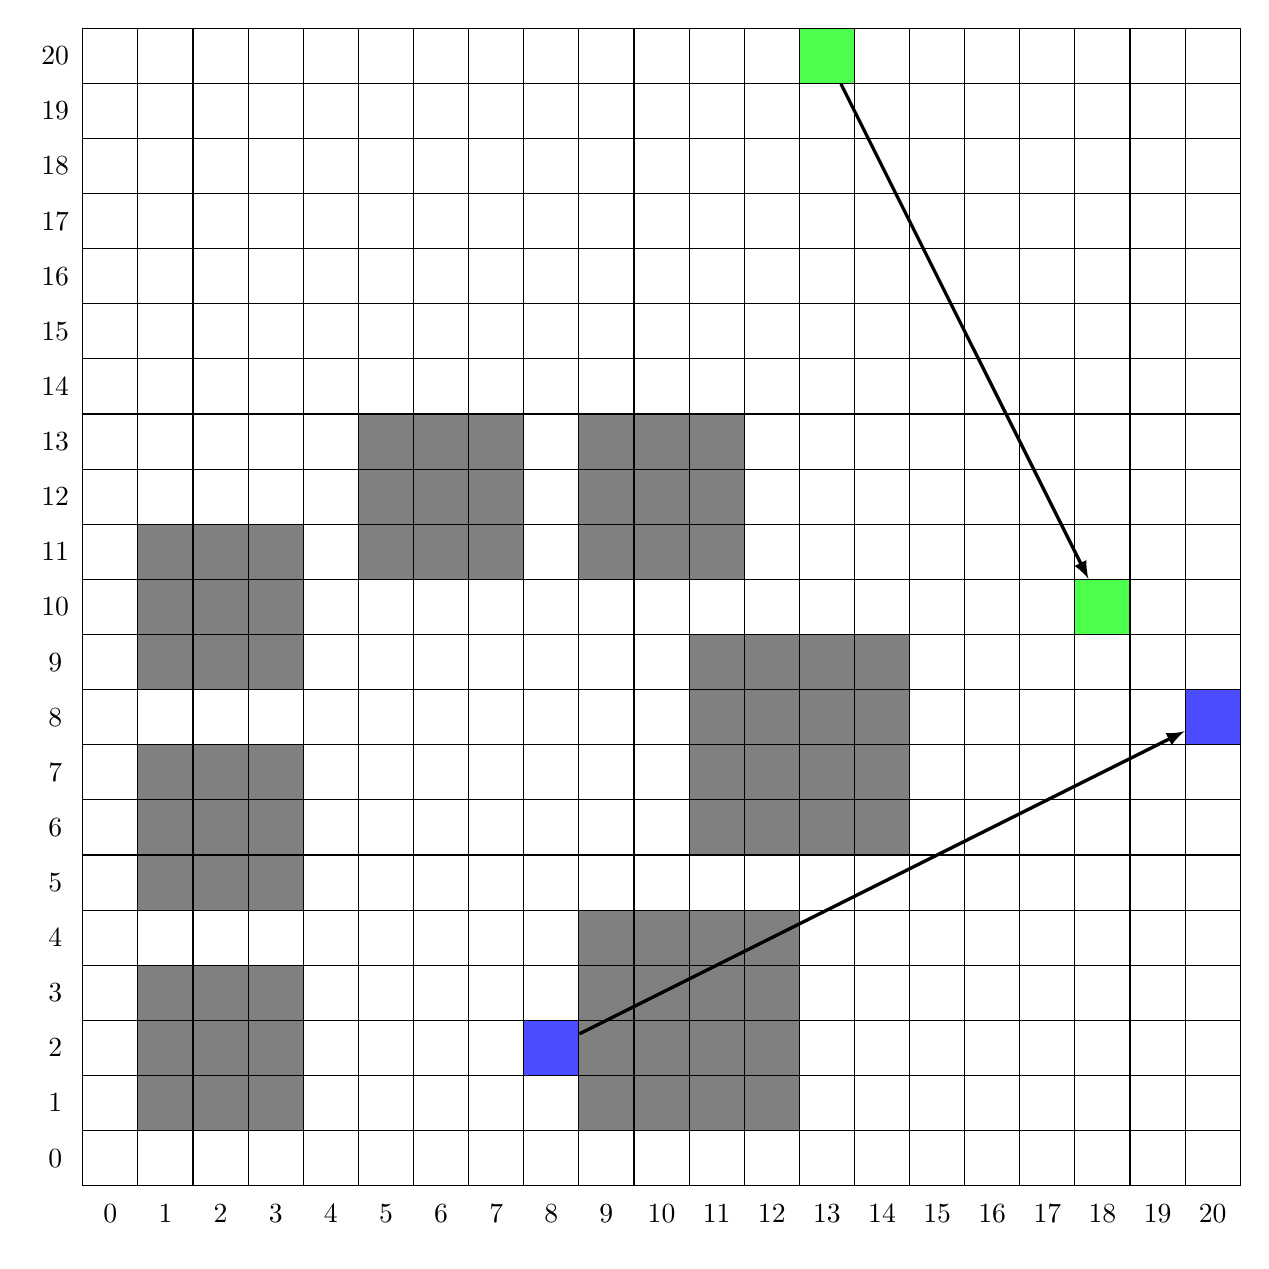
\begin{tikzpicture}[scale=\scale,
	%inner sep=1cm*\scale*\half,
	inner sep=0,
	minimum size=1cm*\scale,
	>=latex,
	pins/.style={rectangle,draw,fill=brown,font=\scriptsize},
	arrow/.style={->,very thick},
	block/.style={gray}]
	% define the row and column number
	\def \N{21}\def \M{21}
	% blockages
	\blockage{11}{6}{14}{9}
	\blockage{9}{1}{12}{4}
	\blockage{1}{1}{3}{3}
	\blockage{9}{11}{11}{13}
	\blockage{5}{11}{7}{13}
	\blockage{1}{5}{3}{7}
	\blockage{1}{9}{3}{11}
	% nets
	\drawtwopin{Dlt10}{20}{8}{Dlt05_to_Dlt10}{8}{2}{blue!70}
	\drawtwopin{Dlt10}{18}{10}{B2}{13}{20}{green!70}
	\drawgrid{\N}{\M}
	\end{tikzpicture}
	\caption{DAC05\_subproblem\_10}
	\end{figure}
	\clearpage
	\begin{figure}
	\centering
	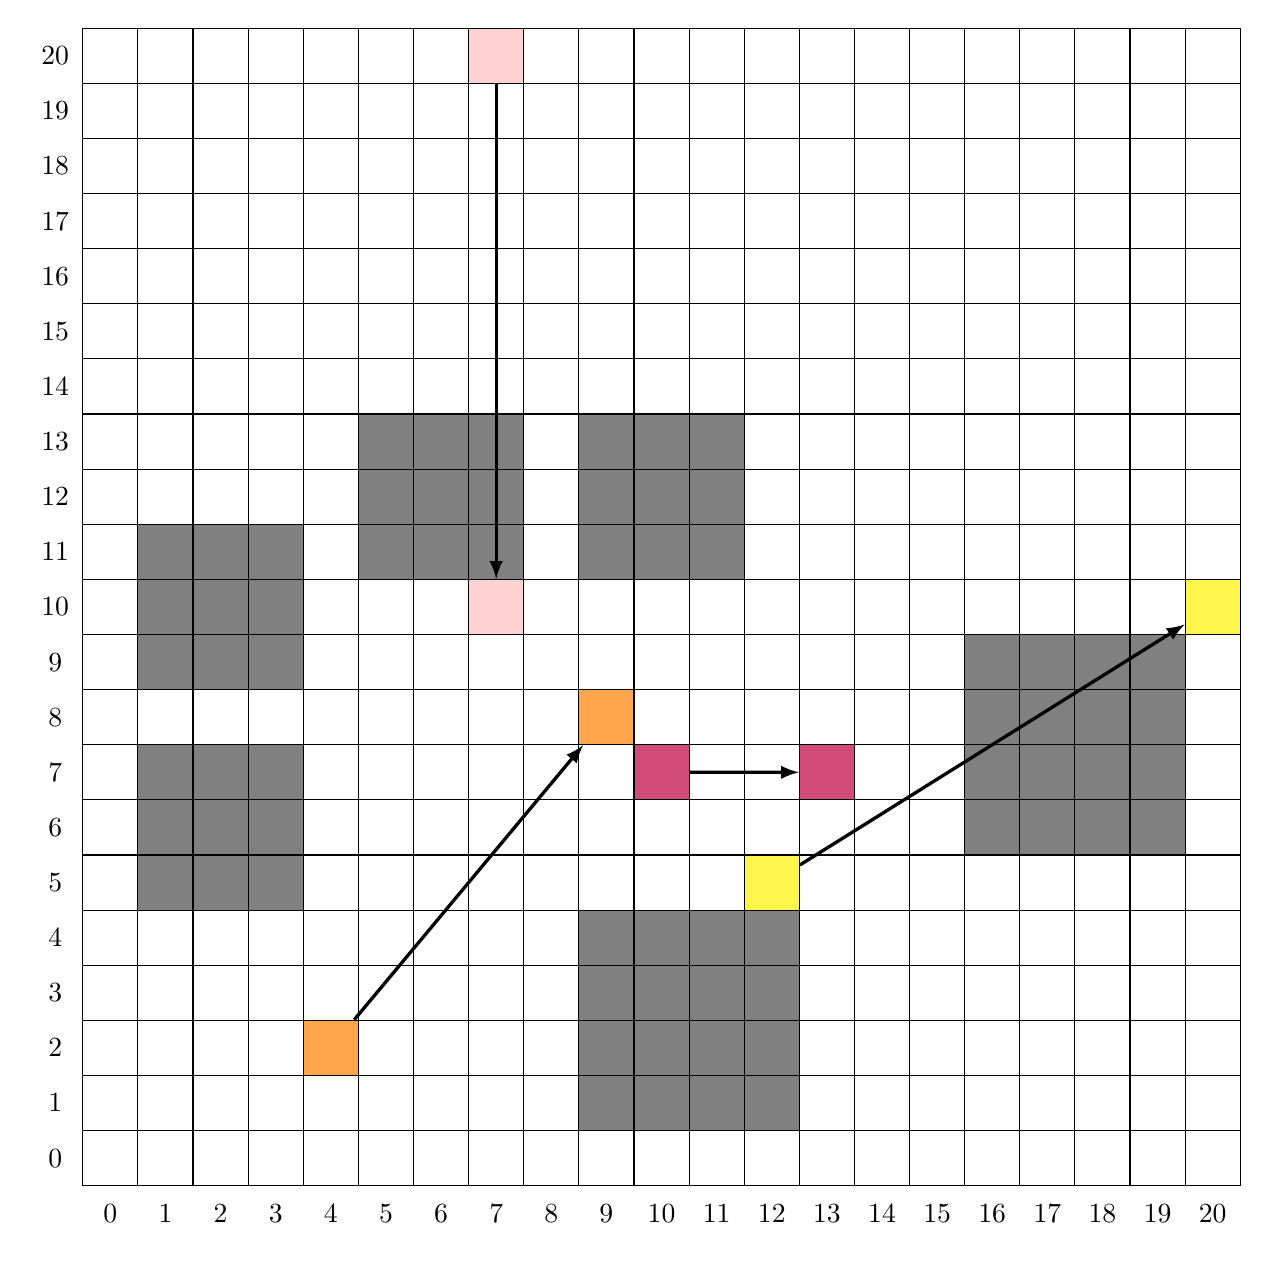
\begin{tikzpicture}[scale=\scale,
	%inner sep=1cm*\scale*\half,
	inner sep=0,
	minimum size=1cm*\scale,
	>=latex,
	pins/.style={rectangle,draw,fill=brown,font=\scriptsize},
	arrow/.style={->,very thick},
	block/.style={gray}]
	% define the row and column number
	\def \N{21}\def \M{21}
	% blockages
	\blockage{9}{1}{12}{4}
	\blockage{16}{6}{19}{9}
	\blockage{9}{11}{11}{13}
	\blockage{5}{11}{7}{13}
	\blockage{1}{5}{3}{7}
	\blockage{1}{9}{3}{11}
	% nets
	\drawtwopin{Dlt11}{9}{8}{Dlt05_to_Dlt11}{4}{2}{orange!70}
	\drawtwopin{Dlt08_to_Dlt16}{13}{7}{Dlt08}{10}{7}{purple!70}
	\drawtwopin{W}{20}{10}{DLT08}{12}{5}{yellow!70}
	\drawtwopin{Dlt11}{7}{10}{B1}{7}{20}{pink!70}
	\drawgrid{\N}{\M}
	\end{tikzpicture}
	\caption{DAC05\_subproblem\_11}
	\end{figure}
	\clearpage
	\begin{figure}
	\centering
	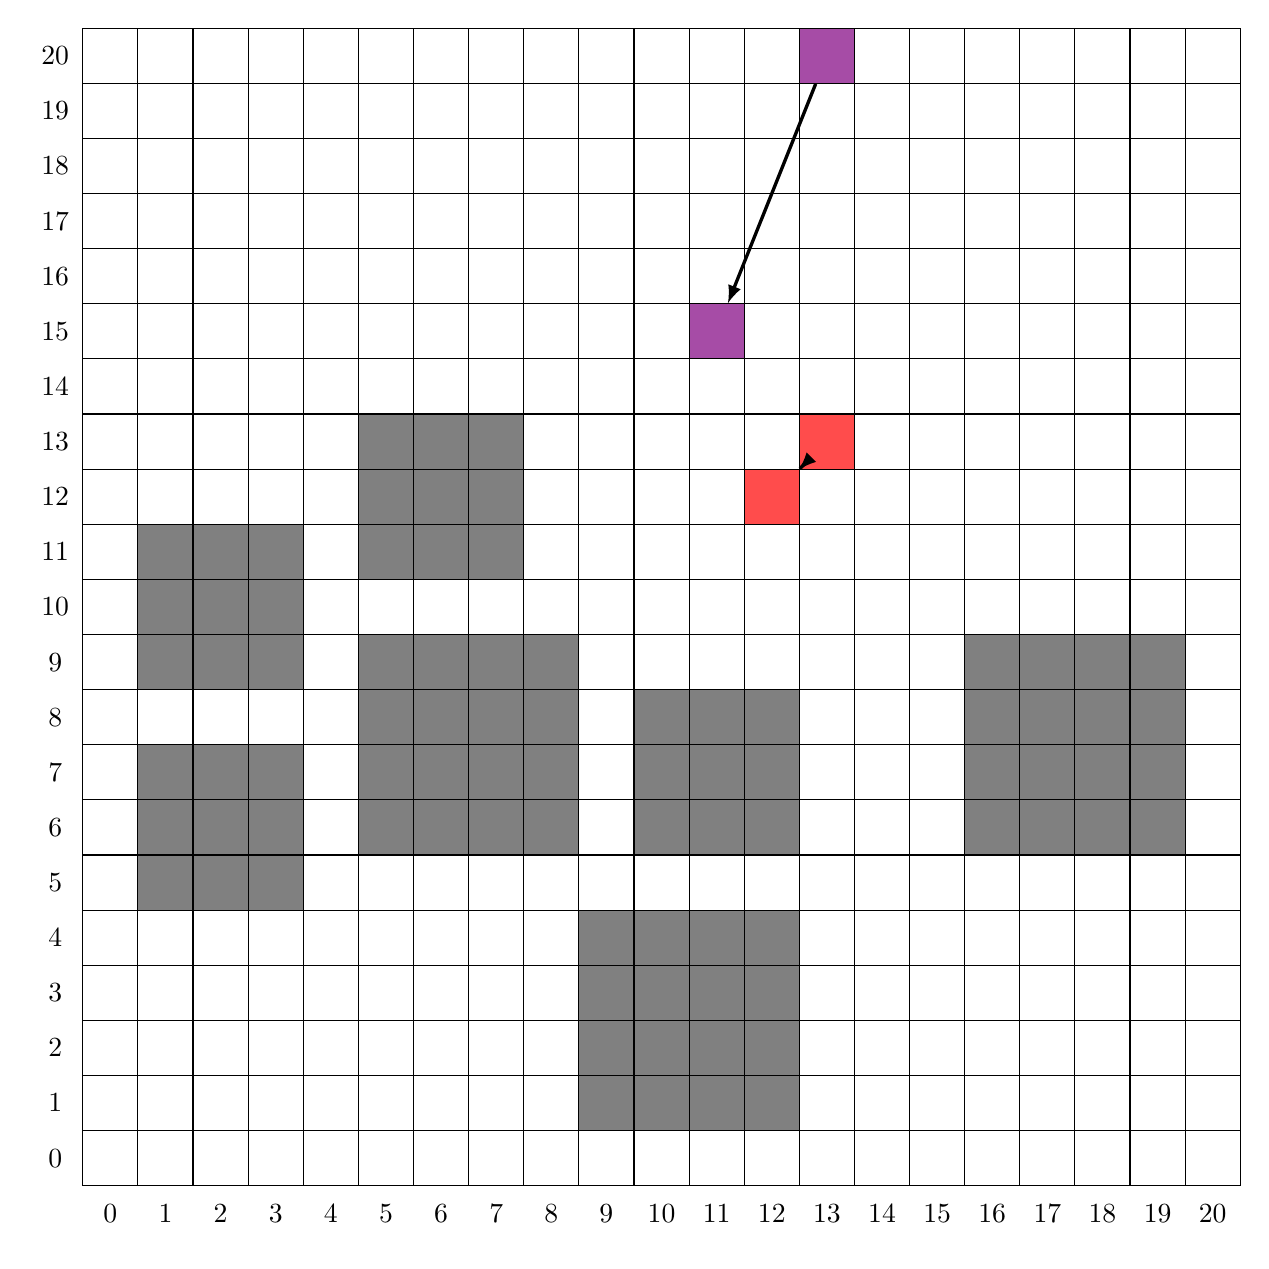
\begin{tikzpicture}[scale=\scale,
	%inner sep=1cm*\scale*\half,
	inner sep=0,
	minimum size=1cm*\scale,
	>=latex,
	pins/.style={rectangle,draw,fill=brown,font=\scriptsize},
	arrow/.style={->,very thick},
	block/.style={gray}]
	% define the row and column number
	\def \N{21}\def \M{21}
	% blockages
	\blockage{9}{1}{12}{4}
	\blockage{16}{6}{19}{9}
	\blockage{5}{6}{8}{9}
	\blockage{5}{11}{7}{13}
	\blockage{1}{5}{3}{7}
	\blockage{1}{9}{3}{11}
	\blockage{10}{6}{12}{8}
	% nets
	\drawtwopin{Dlt12}{11}{15}{B2}{13}{20}{violet!70}
	\drawtwopin{Dlt12}{13}{13}{Dlt06_to_Dlt12}{12}{12}{red!70}
	\drawgrid{\N}{\M}
	\end{tikzpicture}
	\caption{DAC05\_subproblem\_12}
	\end{figure}
	\clearpage
	\begin{figure}
	\centering
	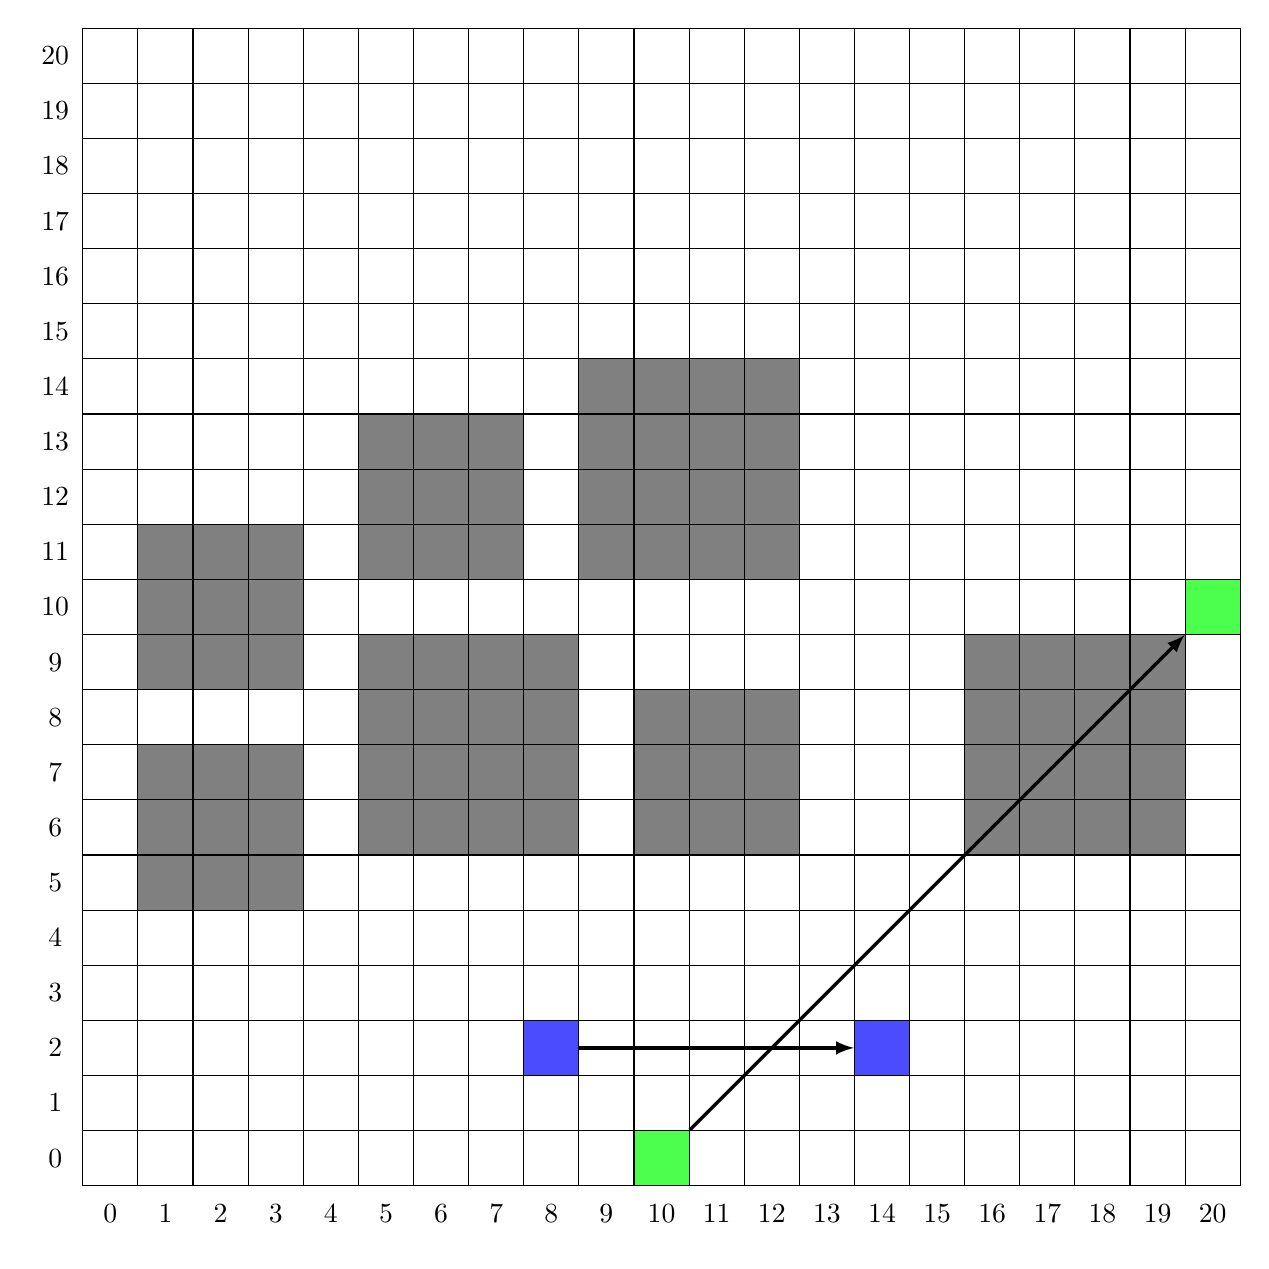
\begin{tikzpicture}[scale=\scale,
	%inner sep=1cm*\scale*\half,
	inner sep=0,
	minimum size=1cm*\scale,
	>=latex,
	pins/.style={rectangle,draw,fill=brown,font=\scriptsize},
	arrow/.style={->,very thick},
	block/.style={gray}]
	% define the row and column number
	\def \N{21}\def \M{21}
	% blockages
	\blockage{16}{6}{19}{9}
	\blockage{5}{6}{8}{9}
	\blockage{9}{11}{12}{14}
	\blockage{5}{11}{7}{13}
	\blockage{1}{5}{3}{7}
	\blockage{1}{9}{3}{11}
	\blockage{10}{6}{12}{8}
	% nets
	\drawtwopin{Dlt09_to_Dlt17}{14}{2}{Dlt09}{8}{2}{blue!70}
	\drawtwopin{W}{20}{10}{Dlt09}{10}{0}{green!70}
	\drawgrid{\N}{\M}
	\end{tikzpicture}
	\caption{DAC05\_subproblem\_13}
	\end{figure}
	\clearpage
	\begin{figure}
	\centering
	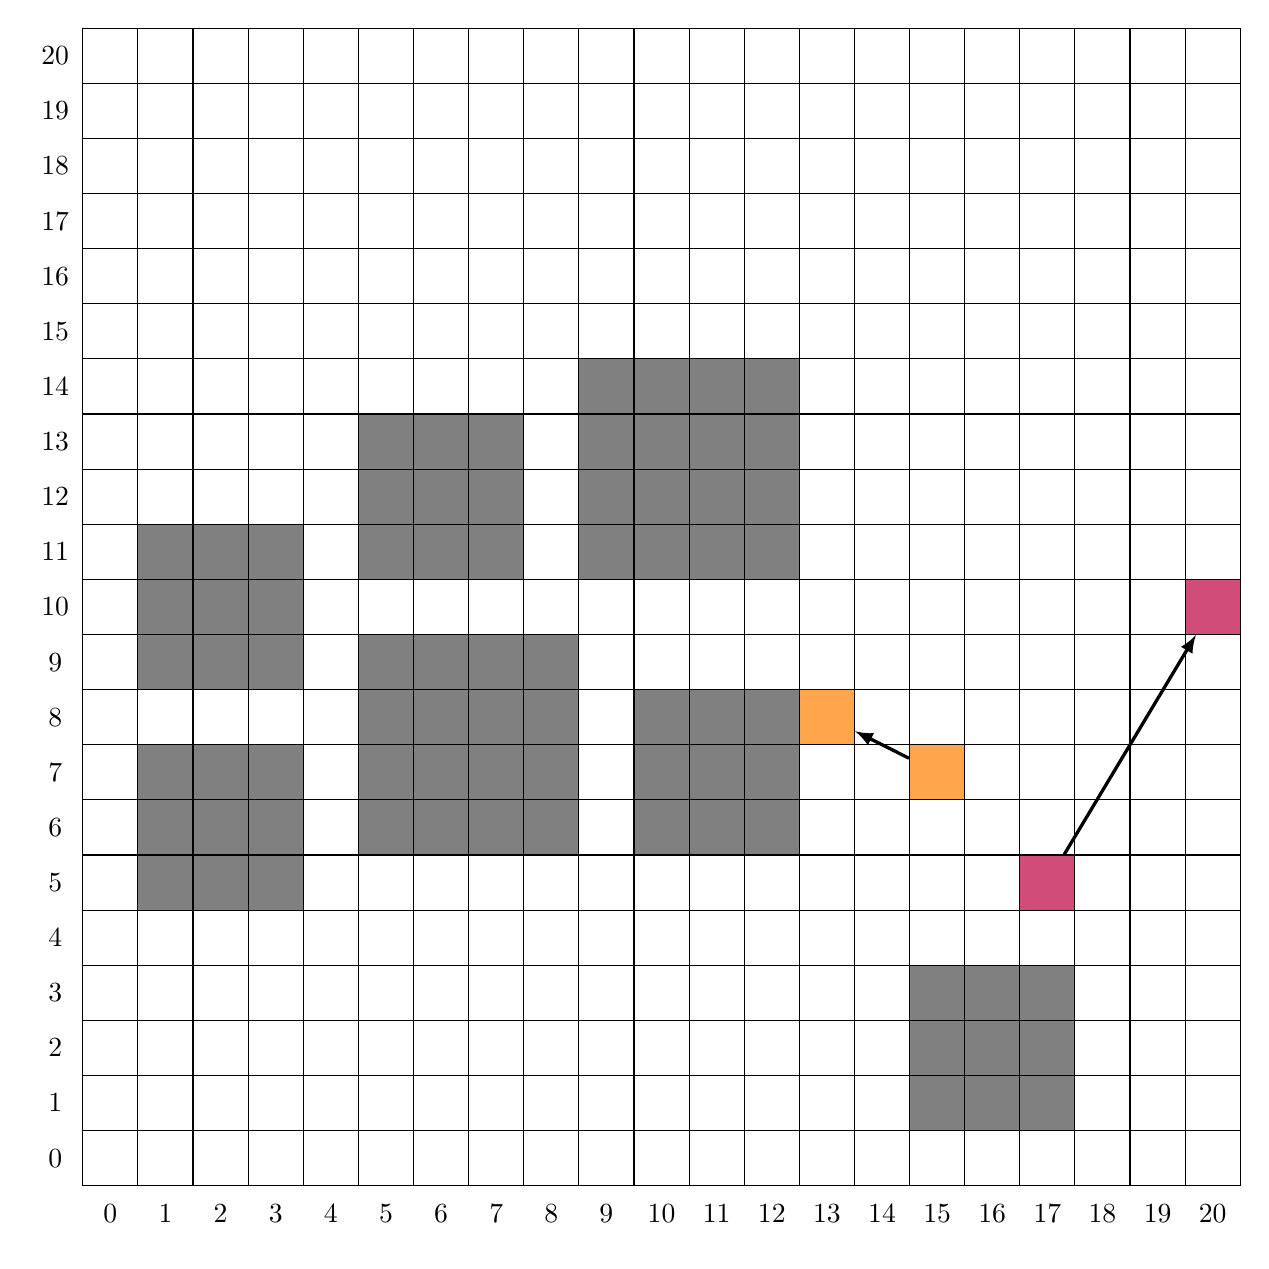
\begin{tikzpicture}[scale=\scale,
	%inner sep=1cm*\scale*\half,
	inner sep=0,
	minimum size=1cm*\scale,
	>=latex,
	pins/.style={rectangle,draw,fill=brown,font=\scriptsize},
	arrow/.style={->,very thick},
	block/.style={gray}]
	% define the row and column number
	\def \N{21}\def \M{21}
	% blockages
	\blockage{5}{6}{8}{9}
	\blockage{9}{11}{12}{14}
	\blockage{5}{11}{7}{13}
	\blockage{1}{5}{3}{7}
	\blockage{1}{9}{3}{11}
	\blockage{10}{6}{12}{8}
	\blockage{15}{1}{17}{3}
	% nets
	\drawtwopin{Dlt10_to_Dlt18}{13}{8}{Dlt10}{15}{7}{orange!70}
	\drawtwopin{W}{20}{10}{Dlt10}{17}{5}{purple!70}
	\drawgrid{\N}{\M}
	\end{tikzpicture}
	\caption{DAC05\_subproblem\_14}
	\end{figure}
	\clearpage
	\begin{figure}
	\centering
	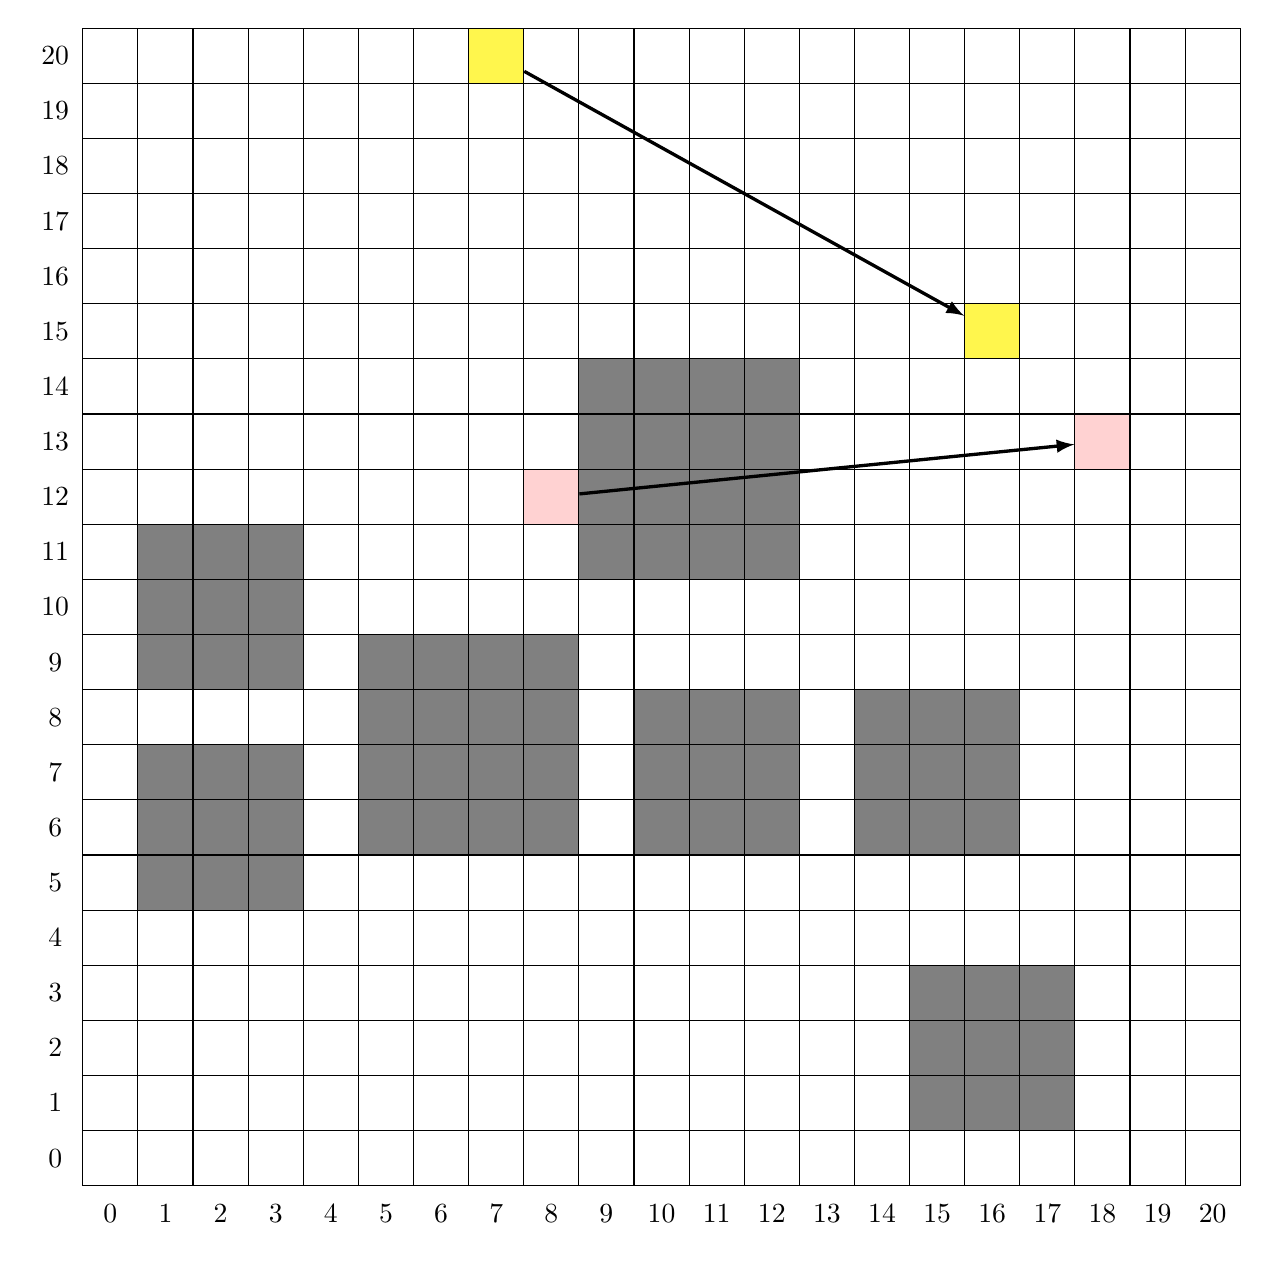
\begin{tikzpicture}[scale=\scale,
	%inner sep=1cm*\scale*\half,
	inner sep=0,
	minimum size=1cm*\scale,
	>=latex,
	pins/.style={rectangle,draw,fill=brown,font=\scriptsize},
	arrow/.style={->,very thick},
	block/.style={gray}]
	% define the row and column number
	\def \N{21}\def \M{21}
	% blockages
	\blockage{5}{6}{8}{9}
	\blockage{9}{11}{12}{14}
	\blockage{1}{5}{3}{7}
	\blockage{1}{9}{3}{11}
	\blockage{10}{6}{12}{8}
	\blockage{15}{1}{17}{3}
	\blockage{14}{6}{16}{8}
	% nets
	\drawtwopin{Dlt13}{16}{15}{B1}{7}{20}{yellow!70}
	\drawtwopin{Dlt13}{18}{13}{Dlt06_to_Dlt13}{8}{12}{pink!70}
	\drawgrid{\N}{\M}
	\end{tikzpicture}
	\caption{DAC05\_subproblem\_15}
	\end{figure}
	\clearpage
	\begin{figure}
	\centering
	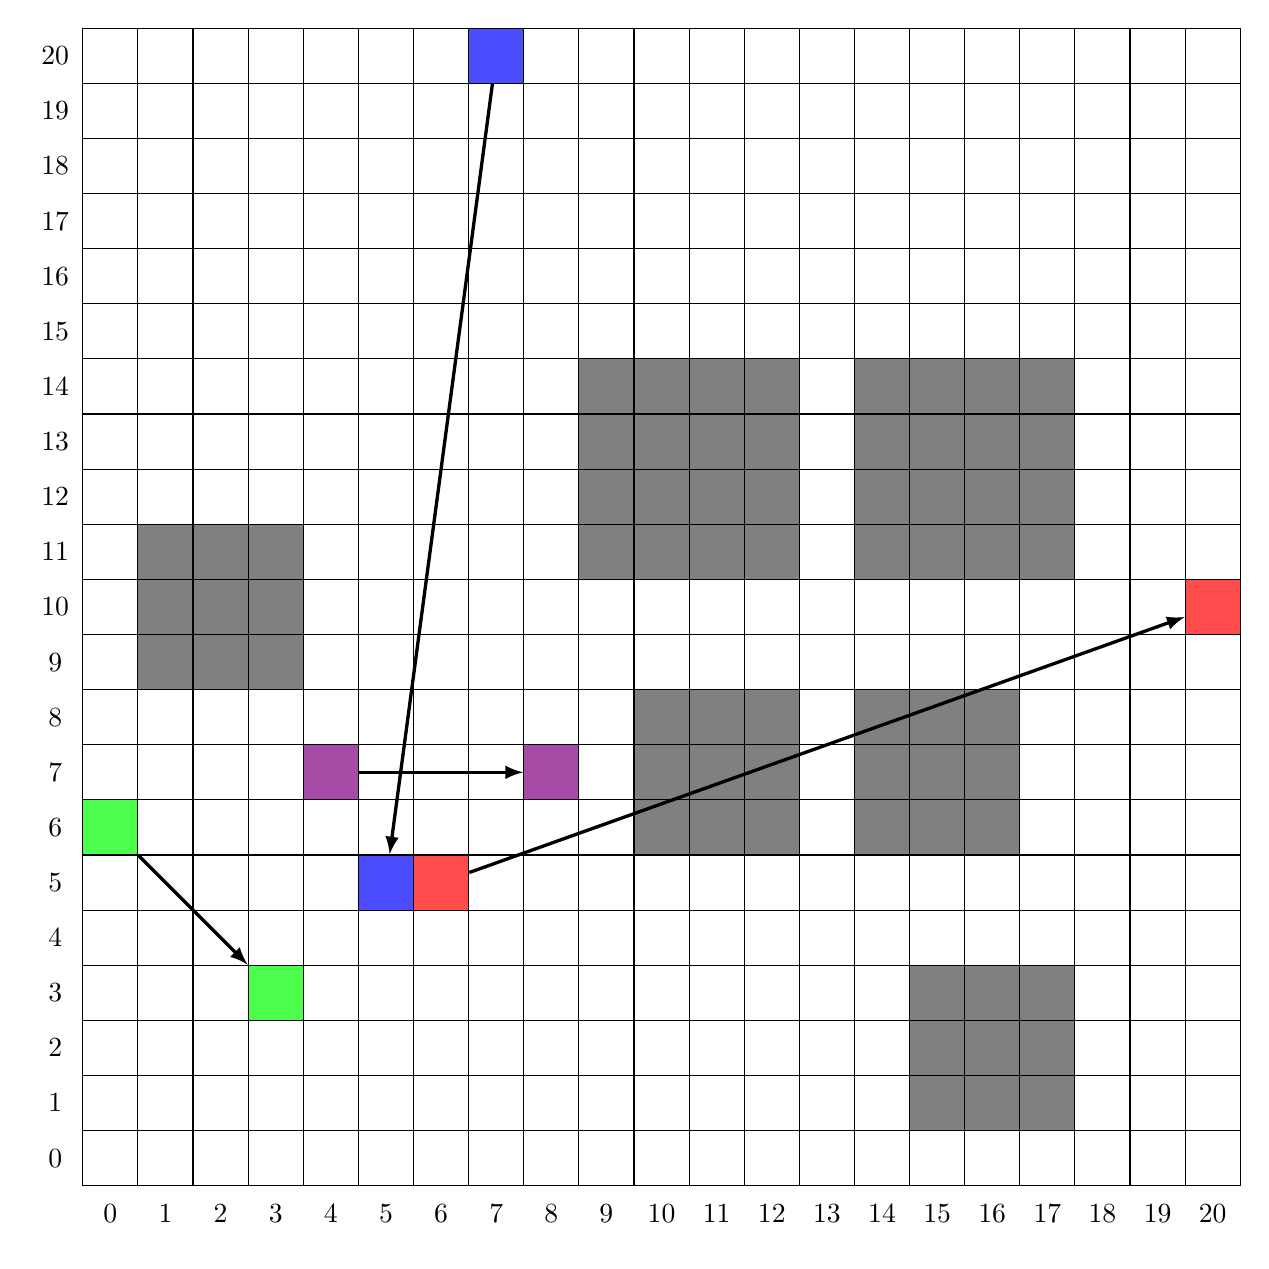
\begin{tikzpicture}[scale=\scale,
	%inner sep=1cm*\scale*\half,
	inner sep=0,
	minimum size=1cm*\scale,
	>=latex,
	pins/.style={rectangle,draw,fill=brown,font=\scriptsize},
	arrow/.style={->,very thick},
	block/.style={gray}]
	% define the row and column number
	\def \N{21}\def \M{21}
	% blockages
	\blockage{9}{11}{12}{14}
	\blockage{14}{11}{17}{14}
	\blockage{1}{9}{3}{11}
	\blockage{10}{6}{12}{8}
	\blockage{15}{1}{17}{3}
	\blockage{14}{6}{16}{8}
	% nets
	\drawtwopin{Dlt11_to_Dlt19}{8}{7}{Dlt11}{4}{7}{violet!70}
	\drawtwopin{W}{20}{10}{Dlt11}{6}{5}{red!70}
	\drawtwopin{Dlt14}{5}{5}{B1}{7}{20}{blue!70}
	\drawtwopin{Dlt14}{3}{3}{Dlt07_to_Dlt14}{0}{6}{green!70}
	\drawgrid{\N}{\M}
	\end{tikzpicture}
	\caption{DAC05\_subproblem\_16}
	\end{figure}
	\clearpage
	\begin{figure}
	\centering
	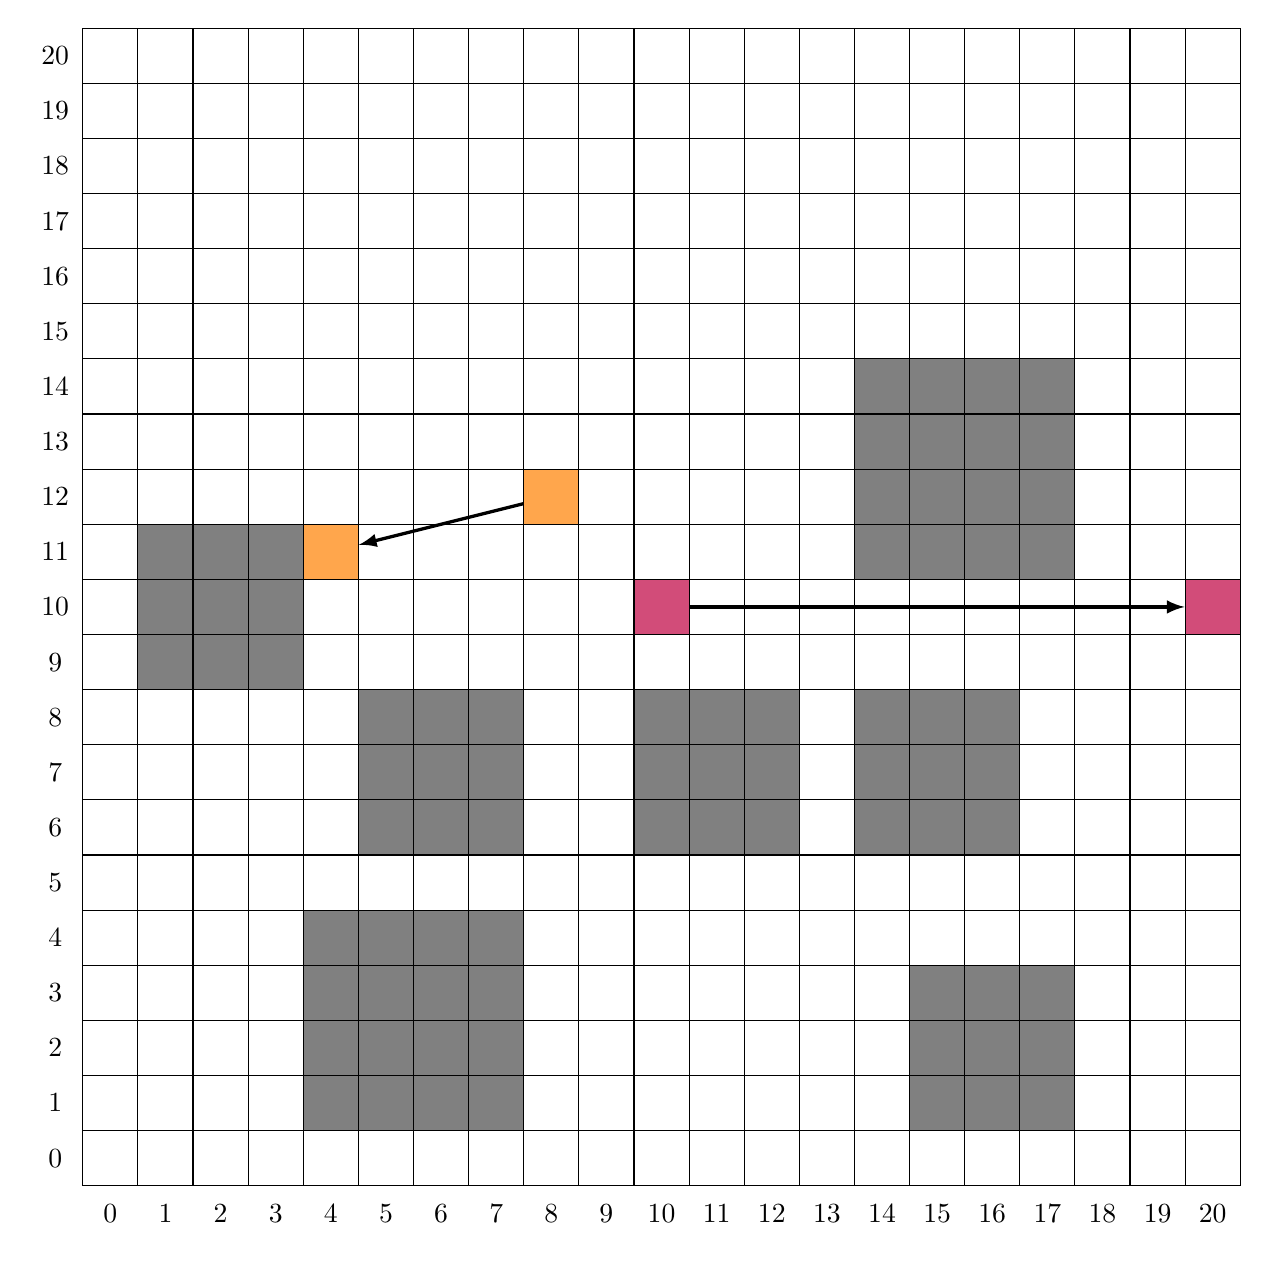
\begin{tikzpicture}[scale=\scale,
	%inner sep=1cm*\scale*\half,
	inner sep=0,
	minimum size=1cm*\scale,
	>=latex,
	pins/.style={rectangle,draw,fill=brown,font=\scriptsize},
	arrow/.style={->,very thick},
	block/.style={gray}]
	% define the row and column number
	\def \N{21}\def \M{21}
	% blockages
	\blockage{14}{11}{17}{14}
	\blockage{4}{1}{7}{4}
	\blockage{1}{9}{3}{11}
	\blockage{10}{6}{12}{8}
	\blockage{15}{1}{17}{3}
	\blockage{14}{6}{16}{8}
	\blockage{5}{6}{7}{8}
	% nets
	\drawtwopin{Dlt12_to_Dlt20}{4}{11}{Dlt12}{8}{12}{orange!70}
	\drawtwopin{W}{20}{10}{Dlt12}{10}{10}{purple!70}
	\drawgrid{\N}{\M}
	\end{tikzpicture}
	\caption{DAC05\_subproblem\_17}
	\end{figure}
	\clearpage
	\begin{figure}
	\centering
	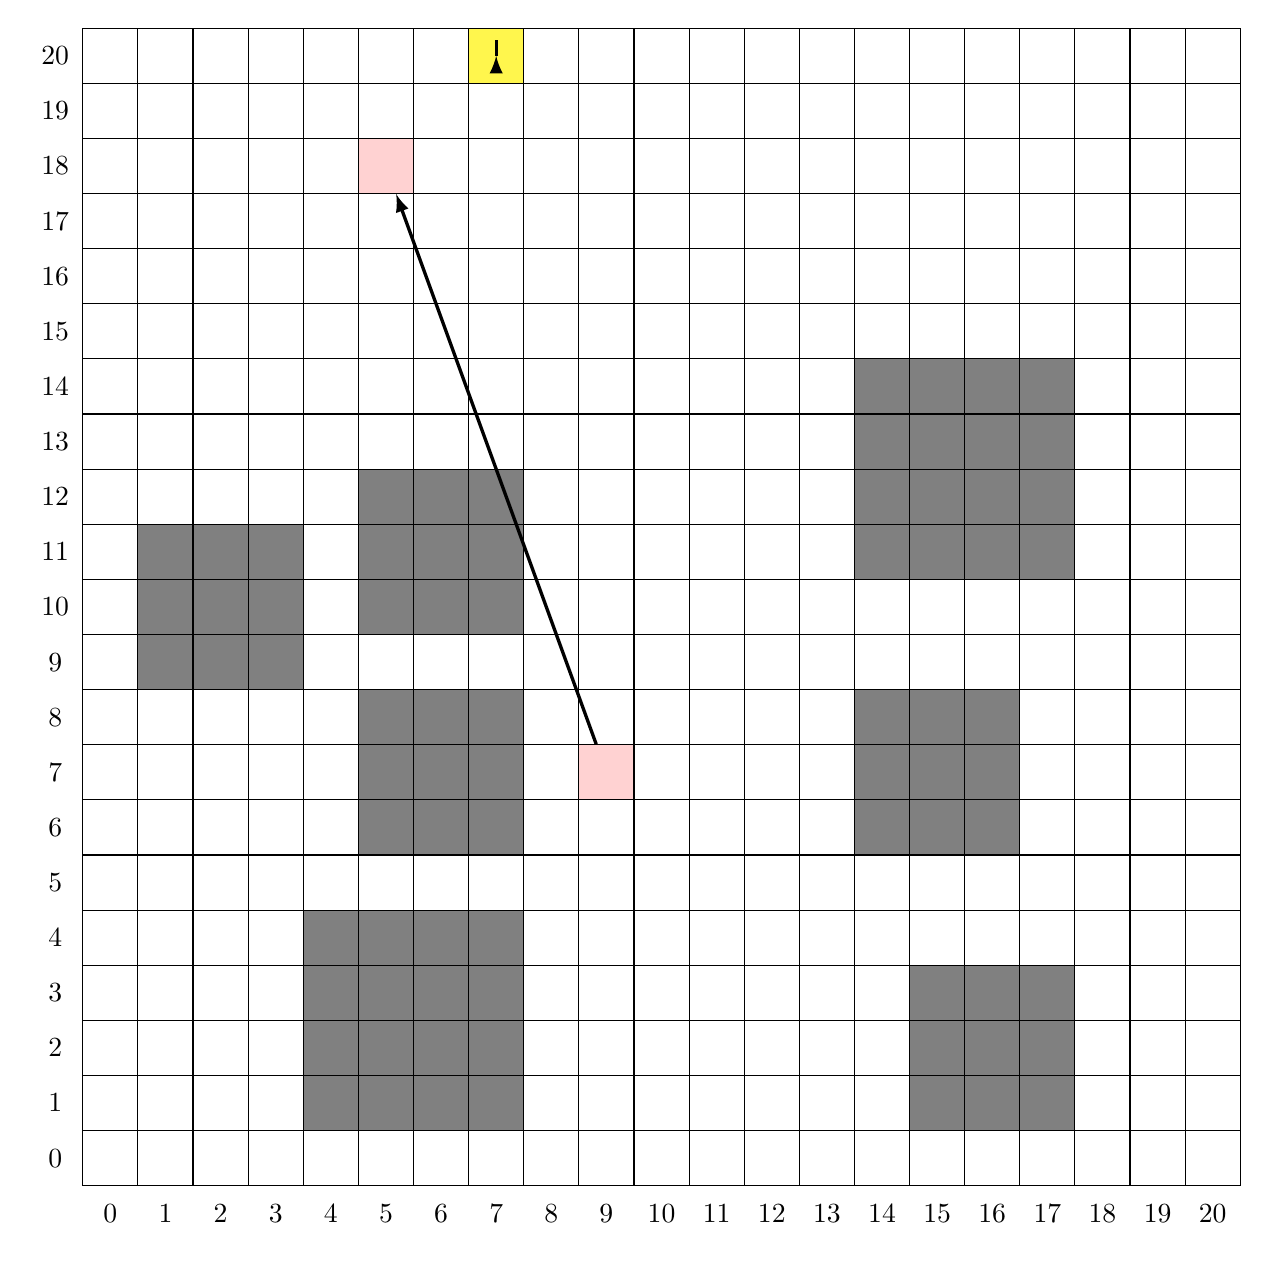
\begin{tikzpicture}[scale=\scale,
	%inner sep=1cm*\scale*\half,
	inner sep=0,
	minimum size=1cm*\scale,
	>=latex,
	pins/.style={rectangle,draw,fill=brown,font=\scriptsize},
	arrow/.style={->,very thick},
	block/.style={gray}]
	% define the row and column number
	\def \N{21}\def \M{21}
	% blockages
	\blockage{14}{11}{17}{14}
	\blockage{4}{1}{7}{4}
	\blockage{1}{9}{3}{11}
	\blockage{15}{1}{17}{3}
	\blockage{14}{6}{16}{8}
	\blockage{5}{6}{7}{8}
	\blockage{5}{10}{7}{12}
	% nets
	\drawtwopin{Dlt16}{7}{20}{B1}{7}{20}{yellow!70}
	\drawtwopin{Dlt16}{5}{18}{Dlt08_to_Dlt16}{9}{7}{pink!70}
	\drawgrid{\N}{\M}
	\end{tikzpicture}
	\caption{DAC05\_subproblem\_18}
	\end{figure}
	\clearpage
	\begin{figure}
	\centering
	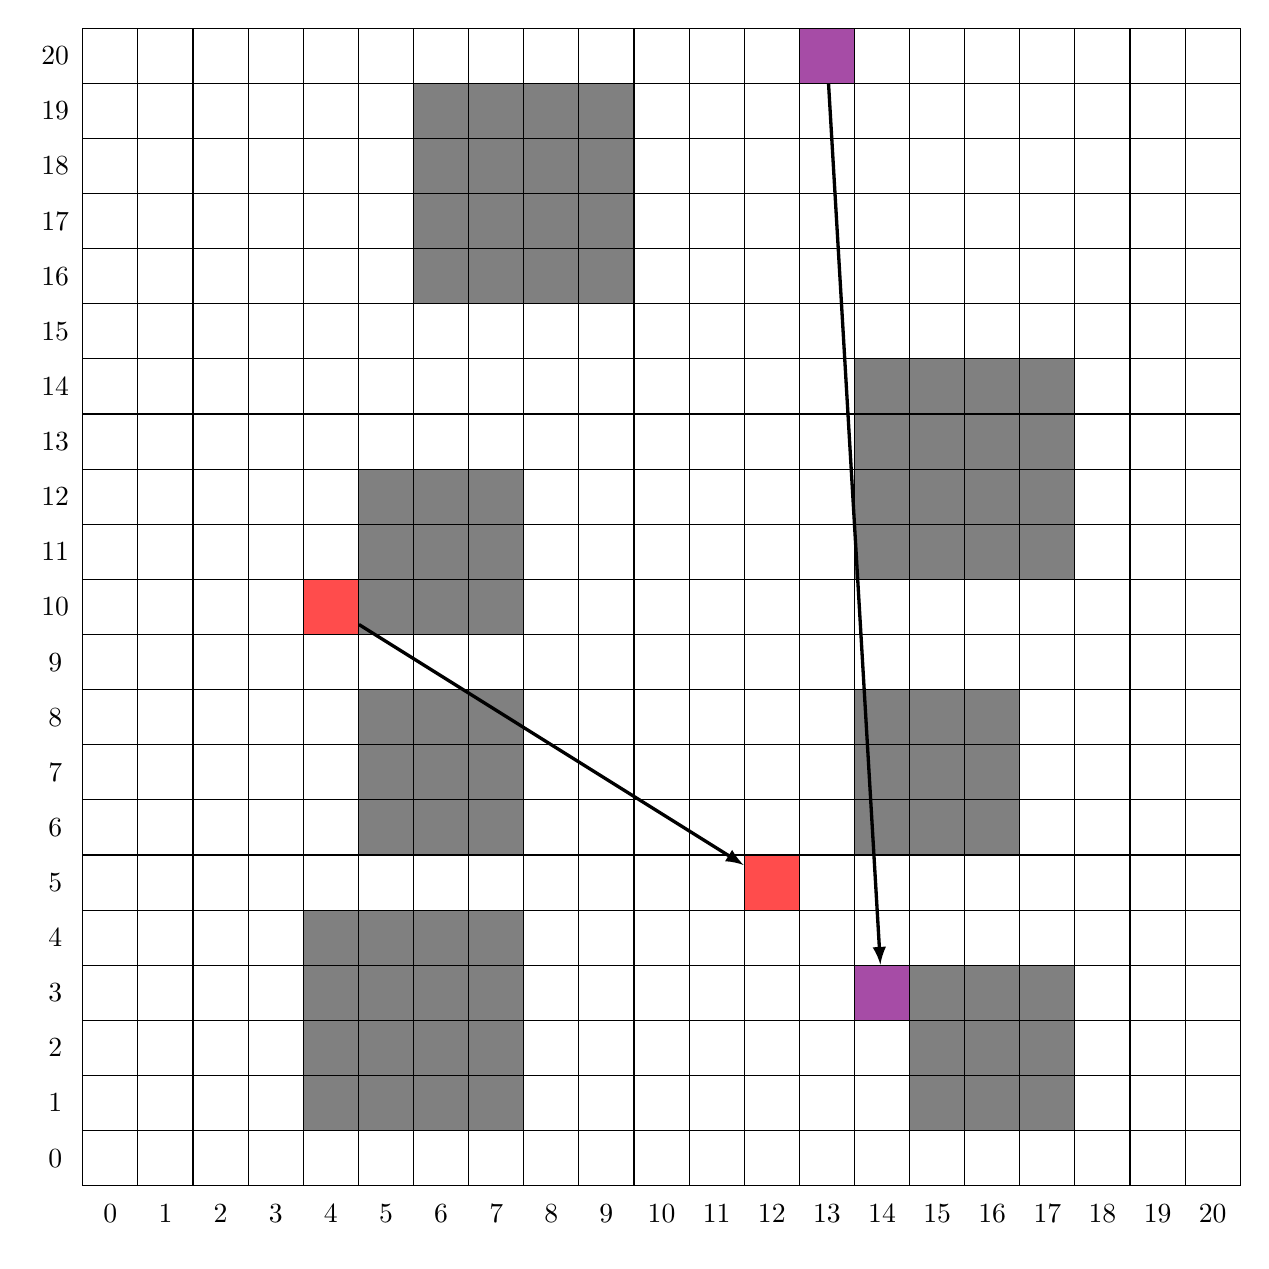
\begin{tikzpicture}[scale=\scale,
	%inner sep=1cm*\scale*\half,
	inner sep=0,
	minimum size=1cm*\scale,
	>=latex,
	pins/.style={rectangle,draw,fill=brown,font=\scriptsize},
	arrow/.style={->,very thick},
	block/.style={gray}]
	% define the row and column number
	\def \N{21}\def \M{21}
	% blockages
	\blockage{14}{11}{17}{14}
	\blockage{4}{1}{7}{4}
	\blockage{6}{16}{9}{19}
	\blockage{15}{1}{17}{3}
	\blockage{14}{6}{16}{8}
	\blockage{5}{6}{7}{8}
	\blockage{5}{10}{7}{12}
	% nets
	\drawtwopin{Dlt15}{14}{3}{B2}{13}{20}{violet!70}
	\drawtwopin{Dlt15}{12}{5}{Dlt07_to_Dlt15}{4}{10}{red!70}
	\drawgrid{\N}{\M}
	\end{tikzpicture}
	\caption{DAC05\_subproblem\_19}
	\end{figure}
	\clearpage
	\begin{figure}
	\centering
	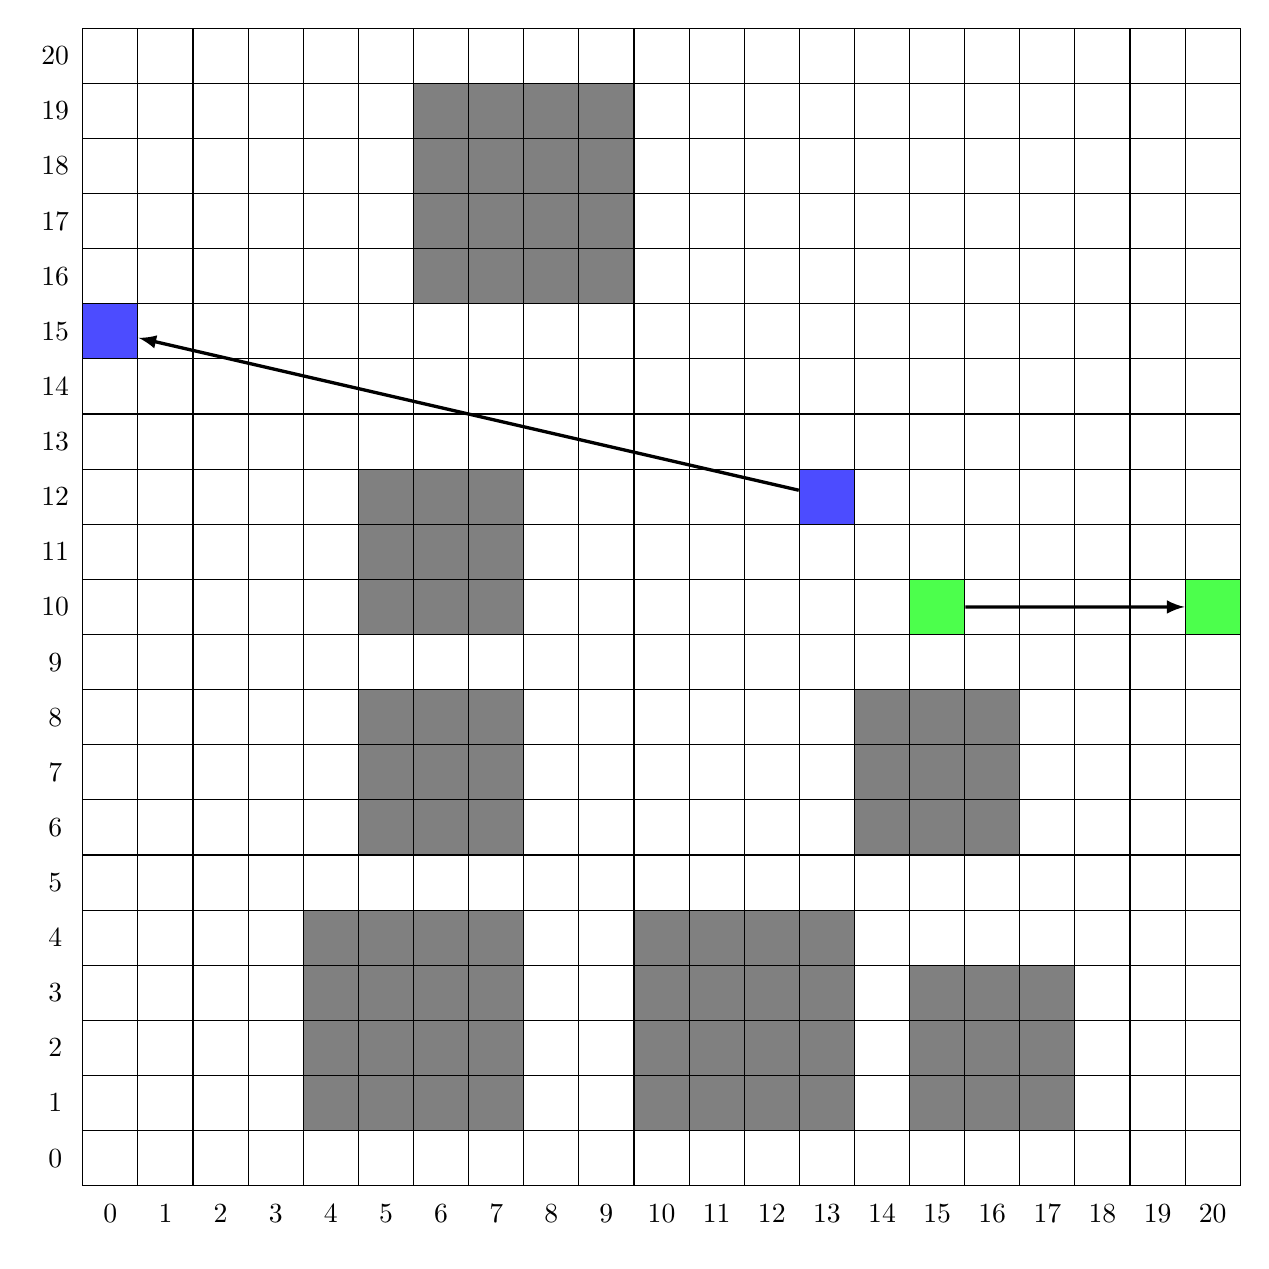
\begin{tikzpicture}[scale=\scale,
	%inner sep=1cm*\scale*\half,
	inner sep=0,
	minimum size=1cm*\scale,
	>=latex,
	pins/.style={rectangle,draw,fill=brown,font=\scriptsize},
	arrow/.style={->,very thick},
	block/.style={gray}]
	% define the row and column number
	\def \N{21}\def \M{21}
	% blockages
	\blockage{4}{1}{7}{4}
	\blockage{10}{1}{13}{4}
	\blockage{6}{16}{9}{19}
	\blockage{15}{1}{17}{3}
	\blockage{14}{6}{16}{8}
	\blockage{5}{6}{7}{8}
	\blockage{5}{10}{7}{12}
	% nets
	\drawtwopin{Dlt13_to_Dlt21}{0}{15}{Dlt13}{13}{12}{blue!70}
	\drawtwopin{W}{20}{10}{Dlt13}{15}{10}{green!70}
	\drawgrid{\N}{\M}
	\end{tikzpicture}
	\caption{DAC05\_subproblem\_20}
	\end{figure}
	\clearpage
	\begin{figure}
	\centering
	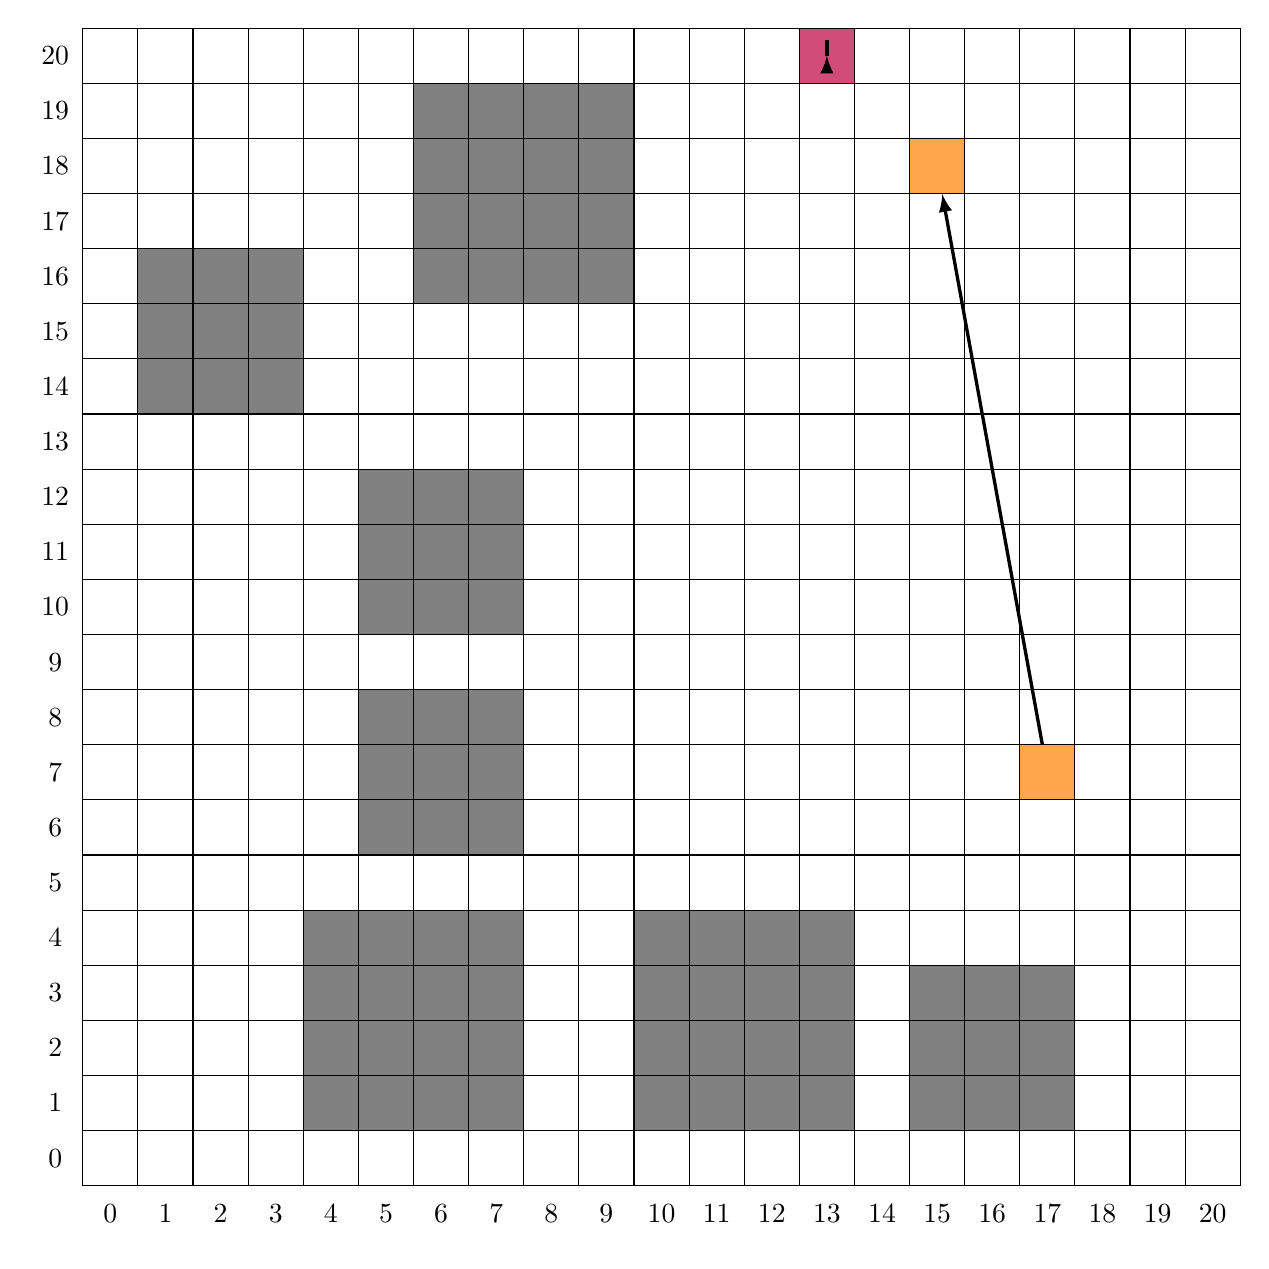
\begin{tikzpicture}[scale=\scale,
	%inner sep=1cm*\scale*\half,
	inner sep=0,
	minimum size=1cm*\scale,
	>=latex,
	pins/.style={rectangle,draw,fill=brown,font=\scriptsize},
	arrow/.style={->,very thick},
	block/.style={gray}]
	% define the row and column number
	\def \N{21}\def \M{21}
	% blockages
	\blockage{4}{1}{7}{4}
	\blockage{10}{1}{13}{4}
	\blockage{6}{16}{9}{19}
	\blockage{15}{1}{17}{3}
	\blockage{5}{6}{7}{8}
	\blockage{5}{10}{7}{12}
	\blockage{1}{14}{3}{16}
	% nets
	\drawtwopin{Dlt18}{15}{18}{Dlt10_to_Dlt18}{17}{7}{orange!70}
	\drawtwopin{Dlt18}{13}{20}{B2}{13}{20}{purple!70}
	\drawgrid{\N}{\M}
	\end{tikzpicture}
	\caption{DAC05\_subproblem\_21}
	\end{figure}
	\clearpage
	\begin{figure}
	\centering
	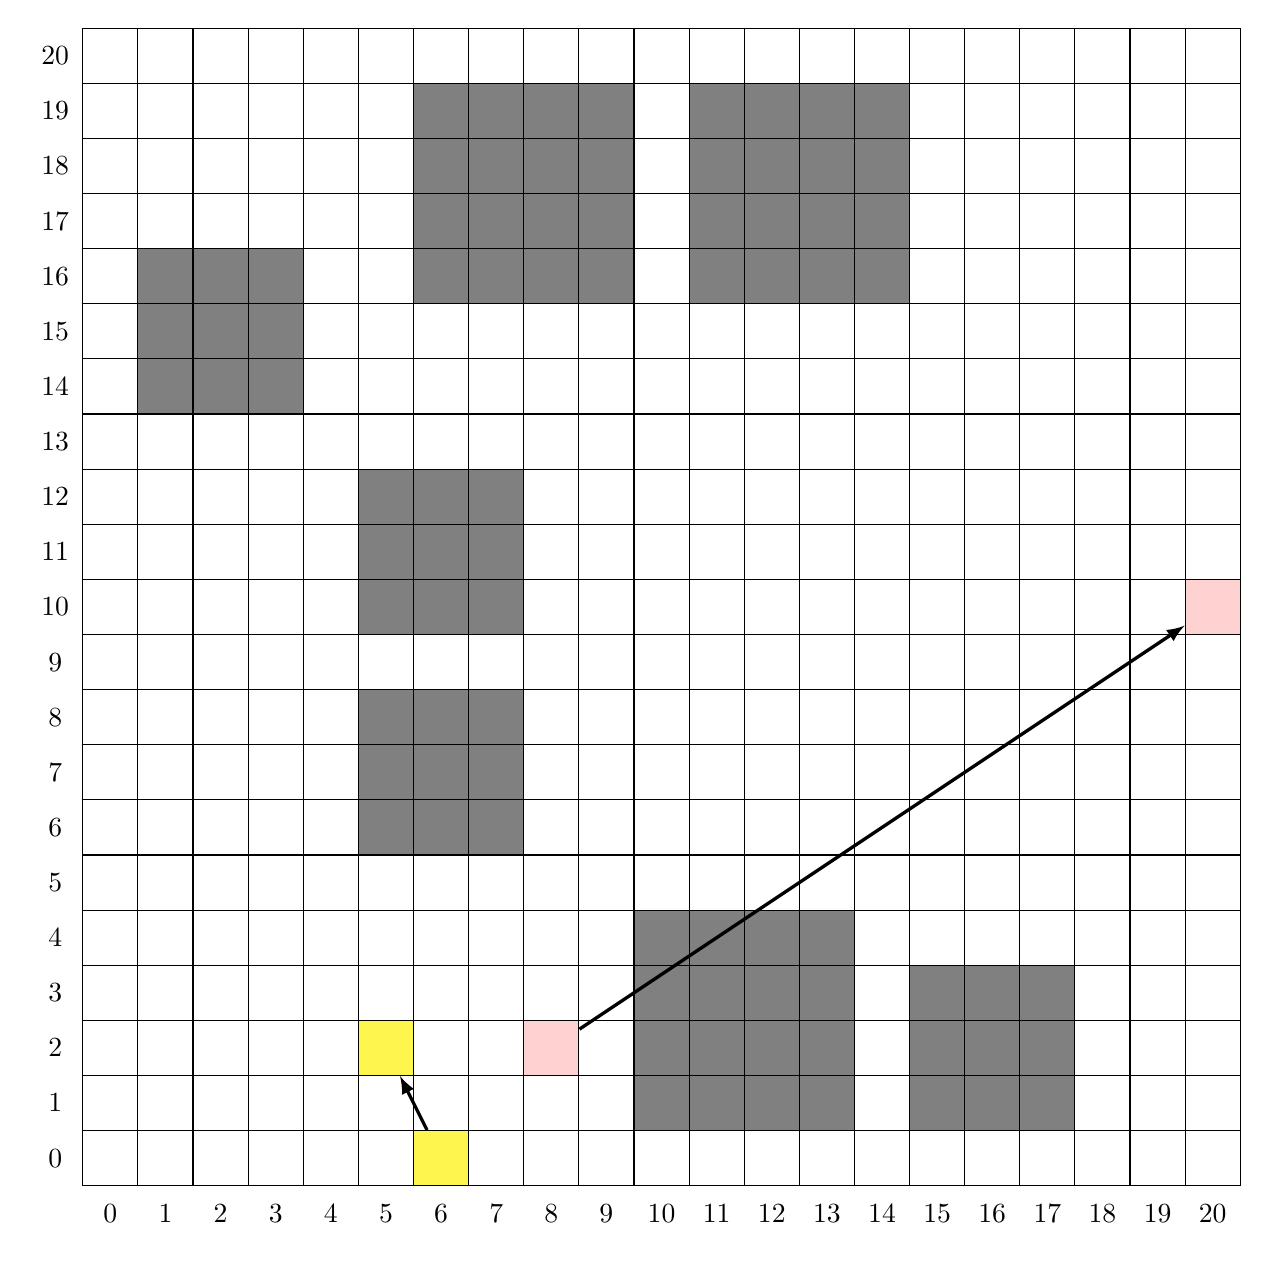
\begin{tikzpicture}[scale=\scale,
	%inner sep=1cm*\scale*\half,
	inner sep=0,
	minimum size=1cm*\scale,
	>=latex,
	pins/.style={rectangle,draw,fill=brown,font=\scriptsize},
	arrow/.style={->,very thick},
	block/.style={gray}]
	% define the row and column number
	\def \N{21}\def \M{21}
	% blockages
	\blockage{10}{1}{13}{4}
	\blockage{6}{16}{9}{19}
	\blockage{11}{16}{14}{19}
	\blockage{15}{1}{17}{3}
	\blockage{5}{6}{7}{8}
	\blockage{5}{10}{7}{12}
	\blockage{1}{14}{3}{16}
	% nets
	\drawtwopin{Dlt14_to_Dlt22}{5}{2}{Dlt14}{6}{0}{yellow!70}
	\drawtwopin{W}{20}{10}{Dlt14}{8}{2}{pink!70}
	\drawgrid{\N}{\M}
	\end{tikzpicture}
	\caption{DAC05\_subproblem\_22}
	\end{figure}
	\clearpage
	\begin{figure}
	\centering
	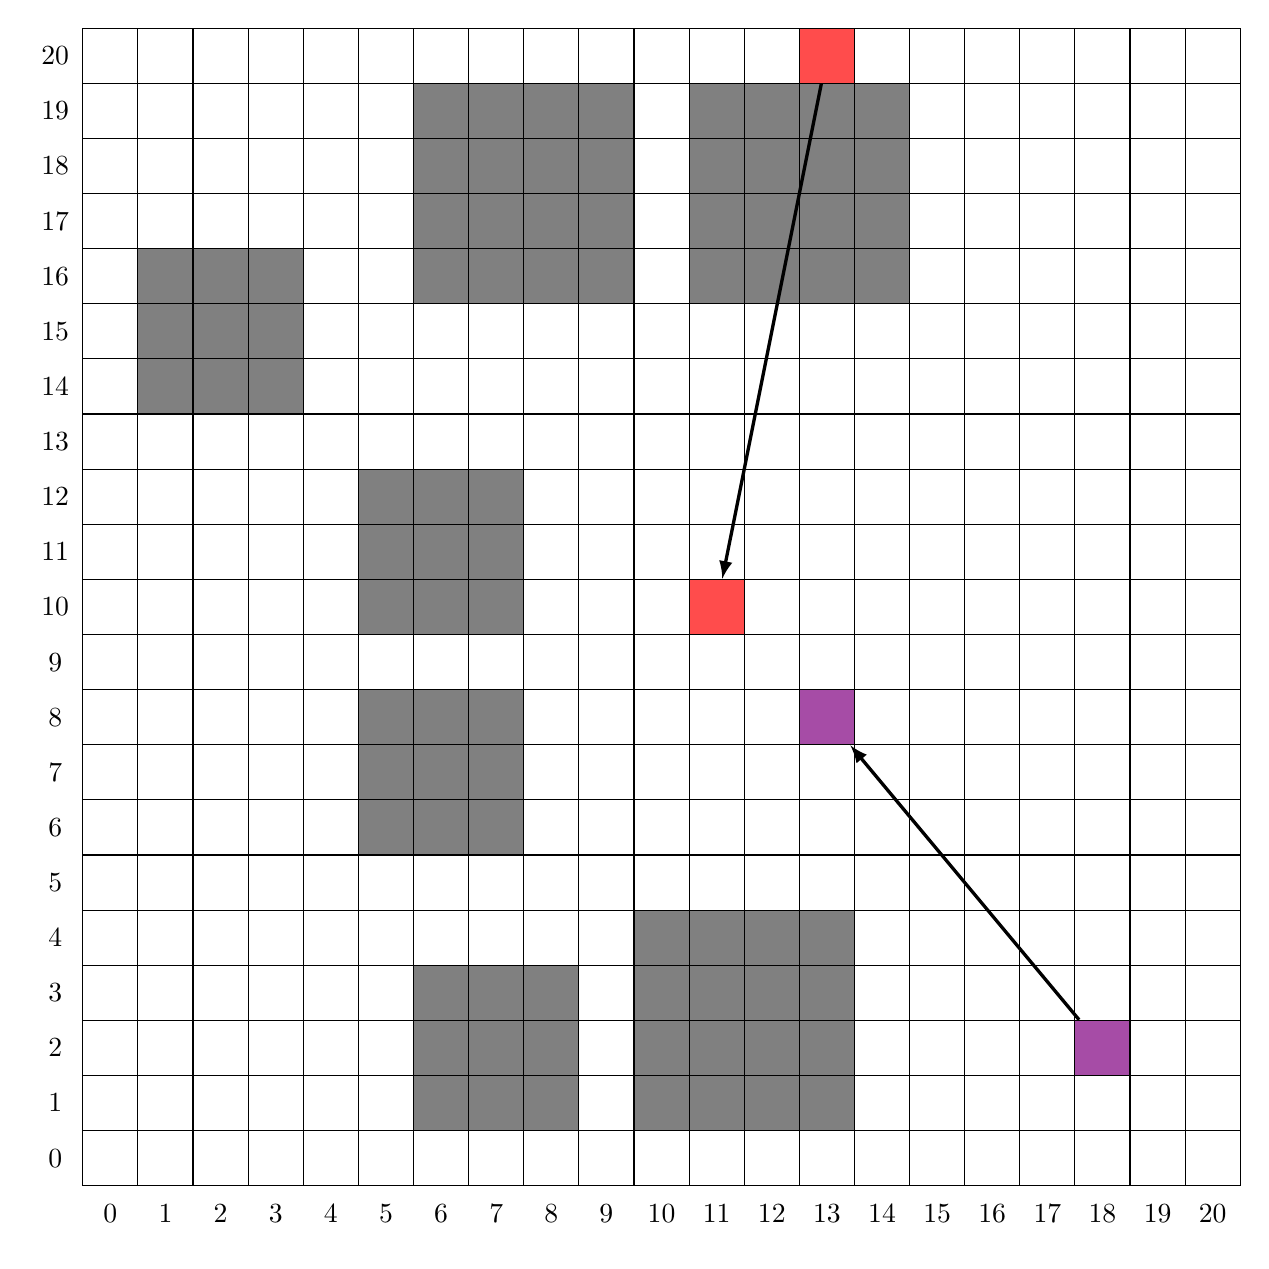
\begin{tikzpicture}[scale=\scale,
	%inner sep=1cm*\scale*\half,
	inner sep=0,
	minimum size=1cm*\scale,
	>=latex,
	pins/.style={rectangle,draw,fill=brown,font=\scriptsize},
	arrow/.style={->,very thick},
	block/.style={gray}]
	% define the row and column number
	\def \N{21}\def \M{21}
	% blockages
	\blockage{10}{1}{13}{4}
	\blockage{6}{16}{9}{19}
	\blockage{11}{16}{14}{19}
	\blockage{5}{6}{7}{8}
	\blockage{5}{10}{7}{12}
	\blockage{1}{14}{3}{16}
	\blockage{6}{1}{8}{3}
	% nets
	\drawtwopin{Dlt17}{13}{8}{Dlt09_to_Dlt17}{18}{2}{violet!70}
	\drawtwopin{Dlt17}{11}{10}{B2}{13}{20}{red!70}
	\drawgrid{\N}{\M}
	\end{tikzpicture}
	\caption{DAC05\_subproblem\_23}
	\end{figure}
	\clearpage
	\begin{figure}
	\centering
	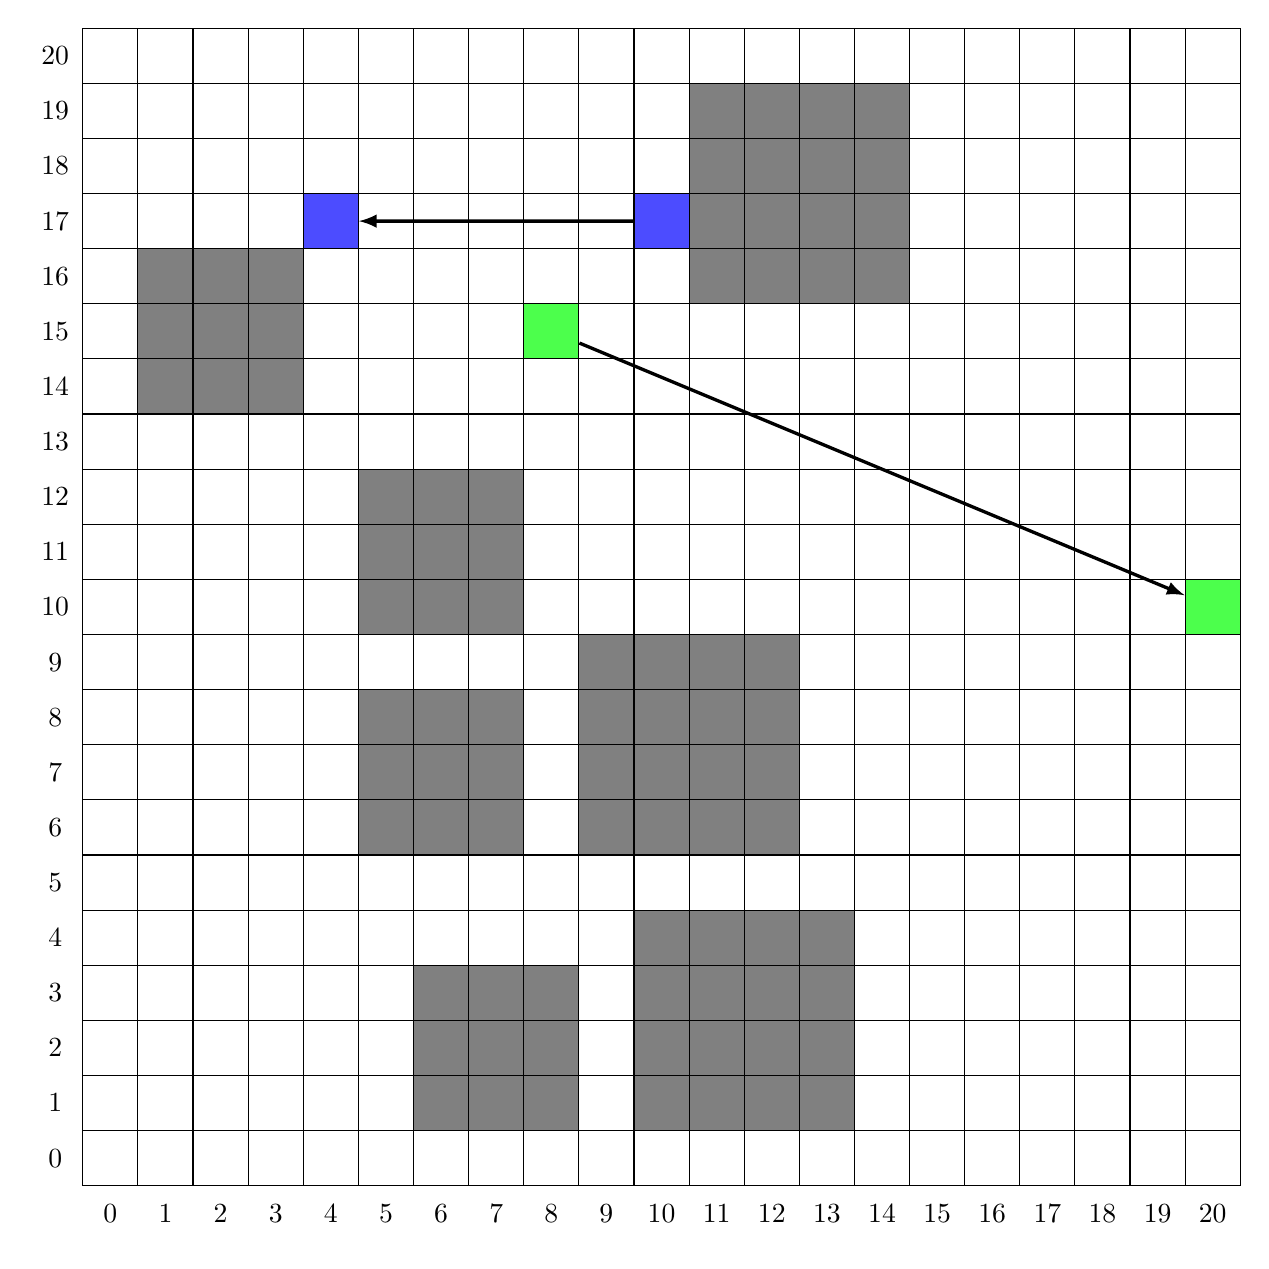
\begin{tikzpicture}[scale=\scale,
	%inner sep=1cm*\scale*\half,
	inner sep=0,
	minimum size=1cm*\scale,
	>=latex,
	pins/.style={rectangle,draw,fill=brown,font=\scriptsize},
	arrow/.style={->,very thick},
	block/.style={gray}]
	% define the row and column number
	\def \N{21}\def \M{21}
	% blockages
	\blockage{10}{1}{13}{4}
	\blockage{9}{6}{12}{9}
	\blockage{11}{16}{14}{19}
	\blockage{5}{6}{7}{8}
	\blockage{5}{10}{7}{12}
	\blockage{1}{14}{3}{16}
	\blockage{6}{1}{8}{3}
	% nets
	\drawtwopin{Dlt16_to_Dlt24}{4}{17}{Dlt16}{10}{17}{blue!70}
	\drawtwopin{W}{20}{10}{Dlt16}{8}{15}{green!70}
	\drawgrid{\N}{\M}
	\end{tikzpicture}
	\caption{DAC05\_subproblem\_24}
	\end{figure}
	\clearpage
	\begin{figure}
	\centering
	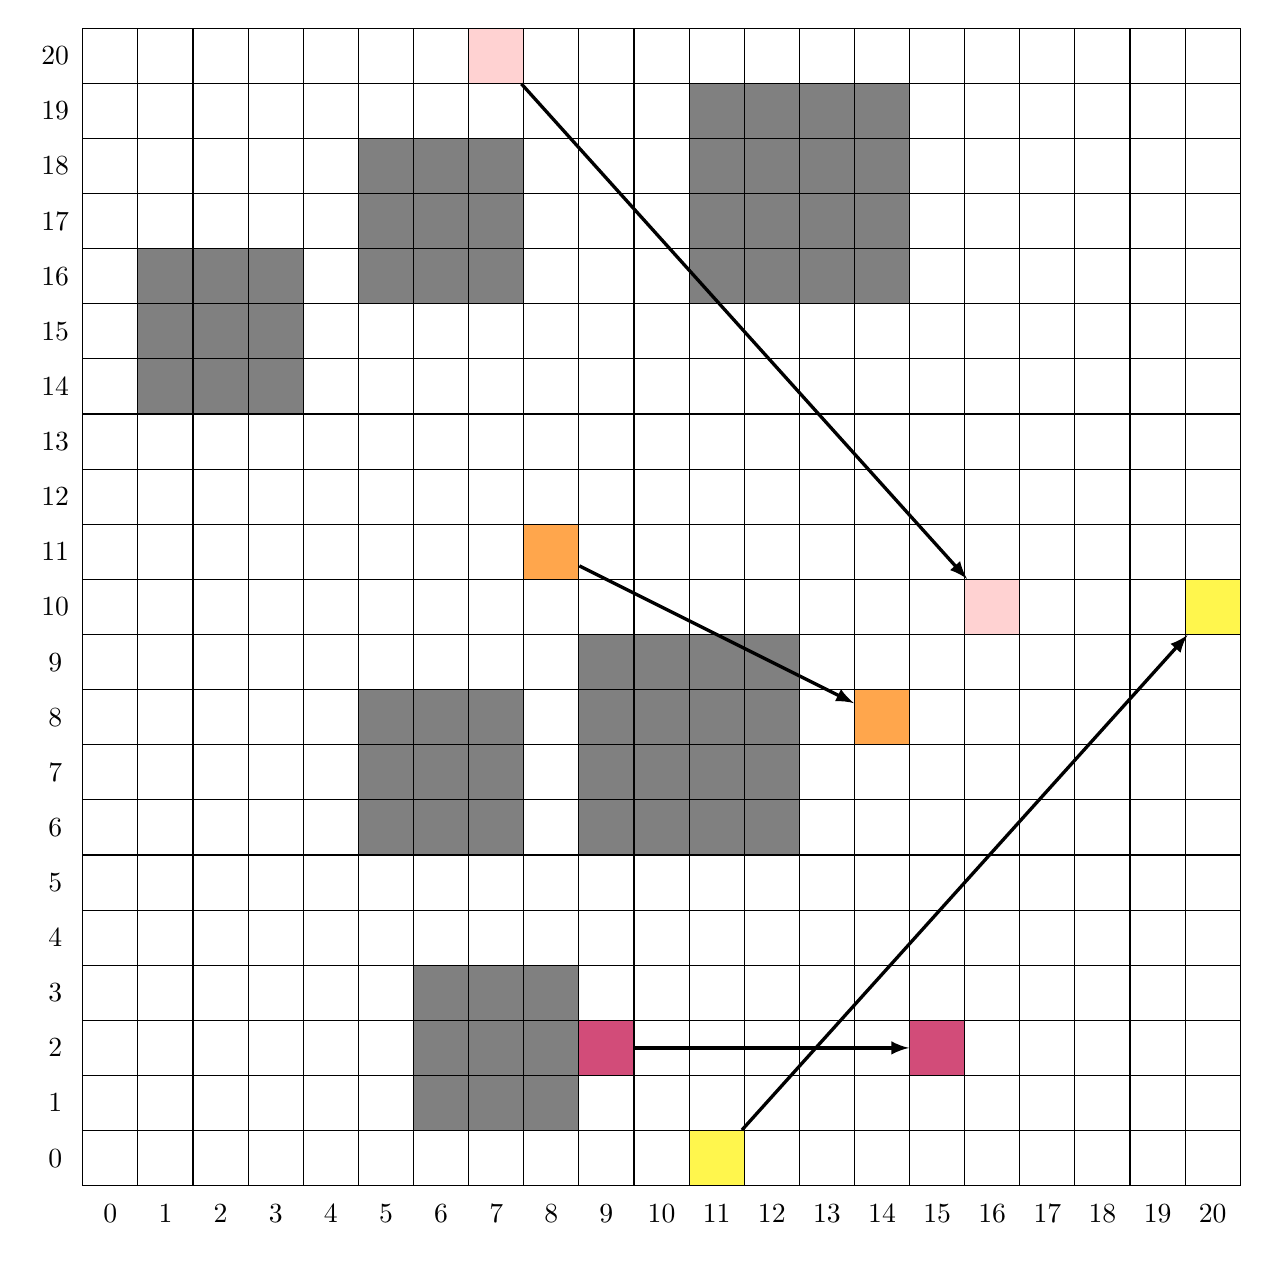
\begin{tikzpicture}[scale=\scale,
	%inner sep=1cm*\scale*\half,
	inner sep=0,
	minimum size=1cm*\scale,
	>=latex,
	pins/.style={rectangle,draw,fill=brown,font=\scriptsize},
	arrow/.style={->,very thick},
	block/.style={gray}]
	% define the row and column number
	\def \N{21}\def \M{21}
	% blockages
	\blockage{9}{6}{12}{9}
	\blockage{11}{16}{14}{19}
	\blockage{5}{6}{7}{8}
	\blockage{1}{14}{3}{16}
	\blockage{6}{1}{8}{3}
	\blockage{5}{16}{7}{18}
	% nets
	\drawtwopin{Dlt20}{14}{8}{Dlt12_to_Dlt20}{8}{11}{orange!70}
	\drawtwopin{Dlt15_to_Dlt23}{15}{2}{Dlt15}{9}{2}{purple!70}
	\drawtwopin{W}{20}{10}{Dlt15}{11}{0}{yellow!70}
	\drawtwopin{Dlt20}{16}{10}{B1}{7}{20}{pink!70}
	\drawgrid{\N}{\M}
	\end{tikzpicture}
	\caption{DAC05\_subproblem\_25}
	\end{figure}
	\clearpage
	\begin{figure}
	\centering
	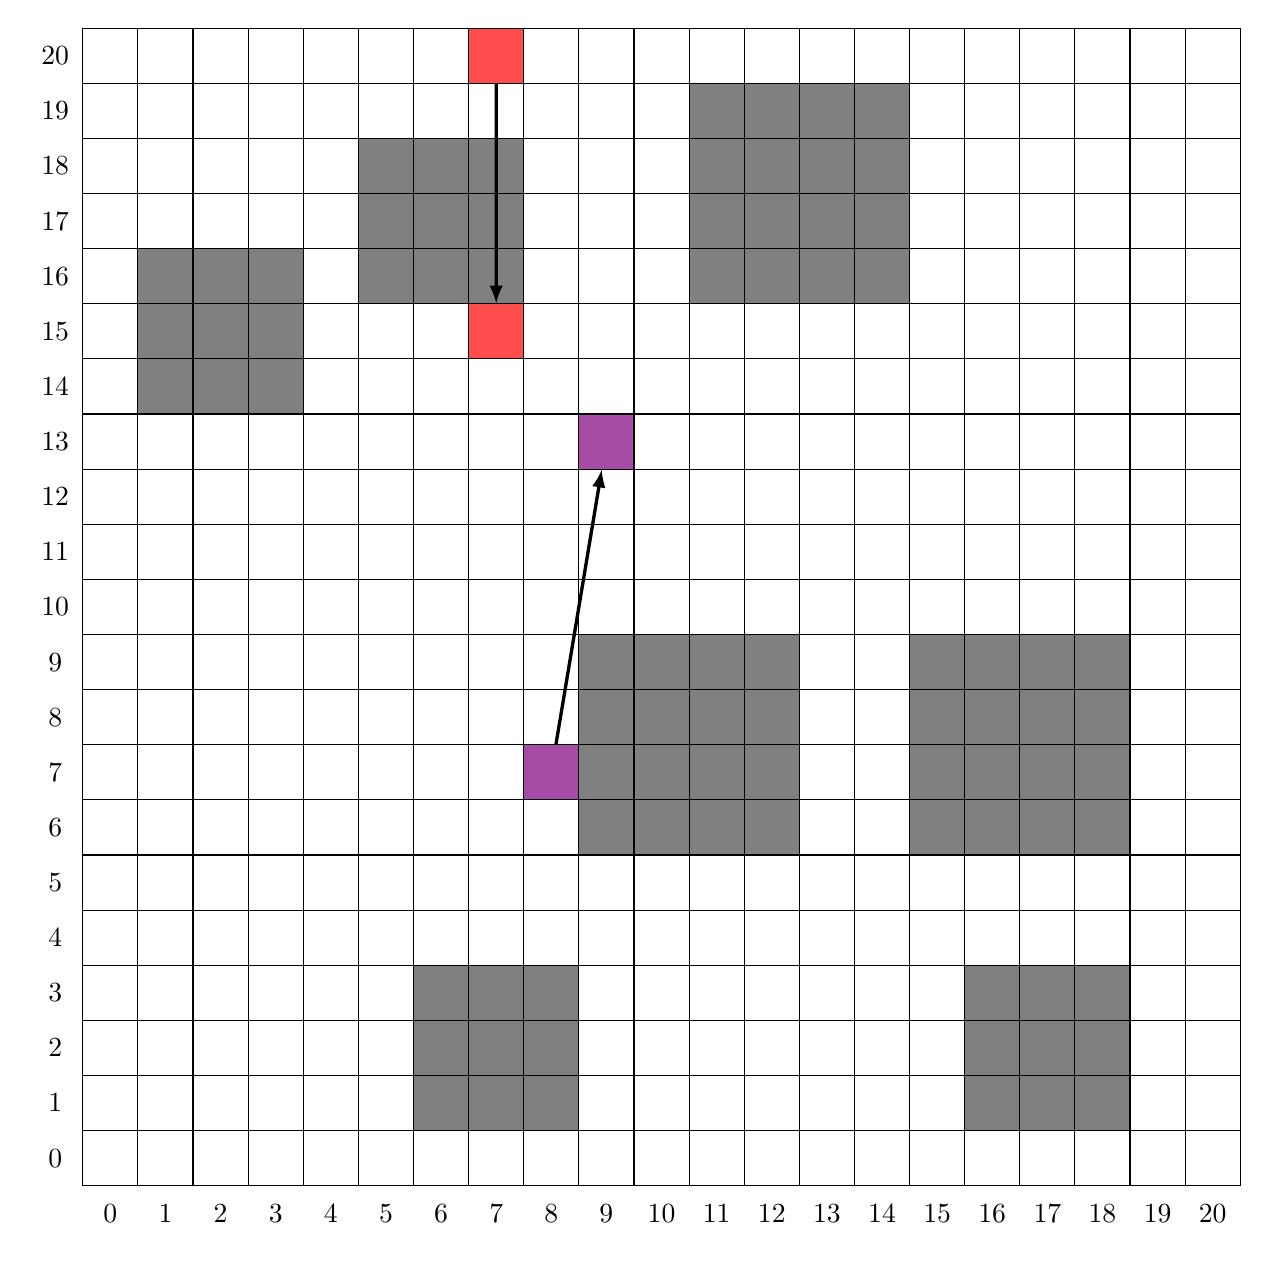
\begin{tikzpicture}[scale=\scale,
	%inner sep=1cm*\scale*\half,
	inner sep=0,
	minimum size=1cm*\scale,
	>=latex,
	pins/.style={rectangle,draw,fill=brown,font=\scriptsize},
	arrow/.style={->,very thick},
	block/.style={gray}]
	% define the row and column number
	\def \N{21}\def \M{21}
	% blockages
	\blockage{9}{6}{12}{9}
	\blockage{11}{16}{14}{19}
	\blockage{15}{6}{18}{9}
	\blockage{1}{14}{3}{16}
	\blockage{6}{1}{8}{3}
	\blockage{16}{1}{18}{3}
	\blockage{5}{16}{7}{18}
	% nets
	\drawtwopin{Dlt19}{9}{13}{Dlt11_to_Dlt19}{8}{7}{violet!70}
	\drawtwopin{Dlt19}{7}{15}{B1}{7}{20}{red!70}
	\drawgrid{\N}{\M}
	\end{tikzpicture}
	\caption{DAC05\_subproblem\_26}
	\end{figure}
	\clearpage
	\begin{figure}
	\centering
	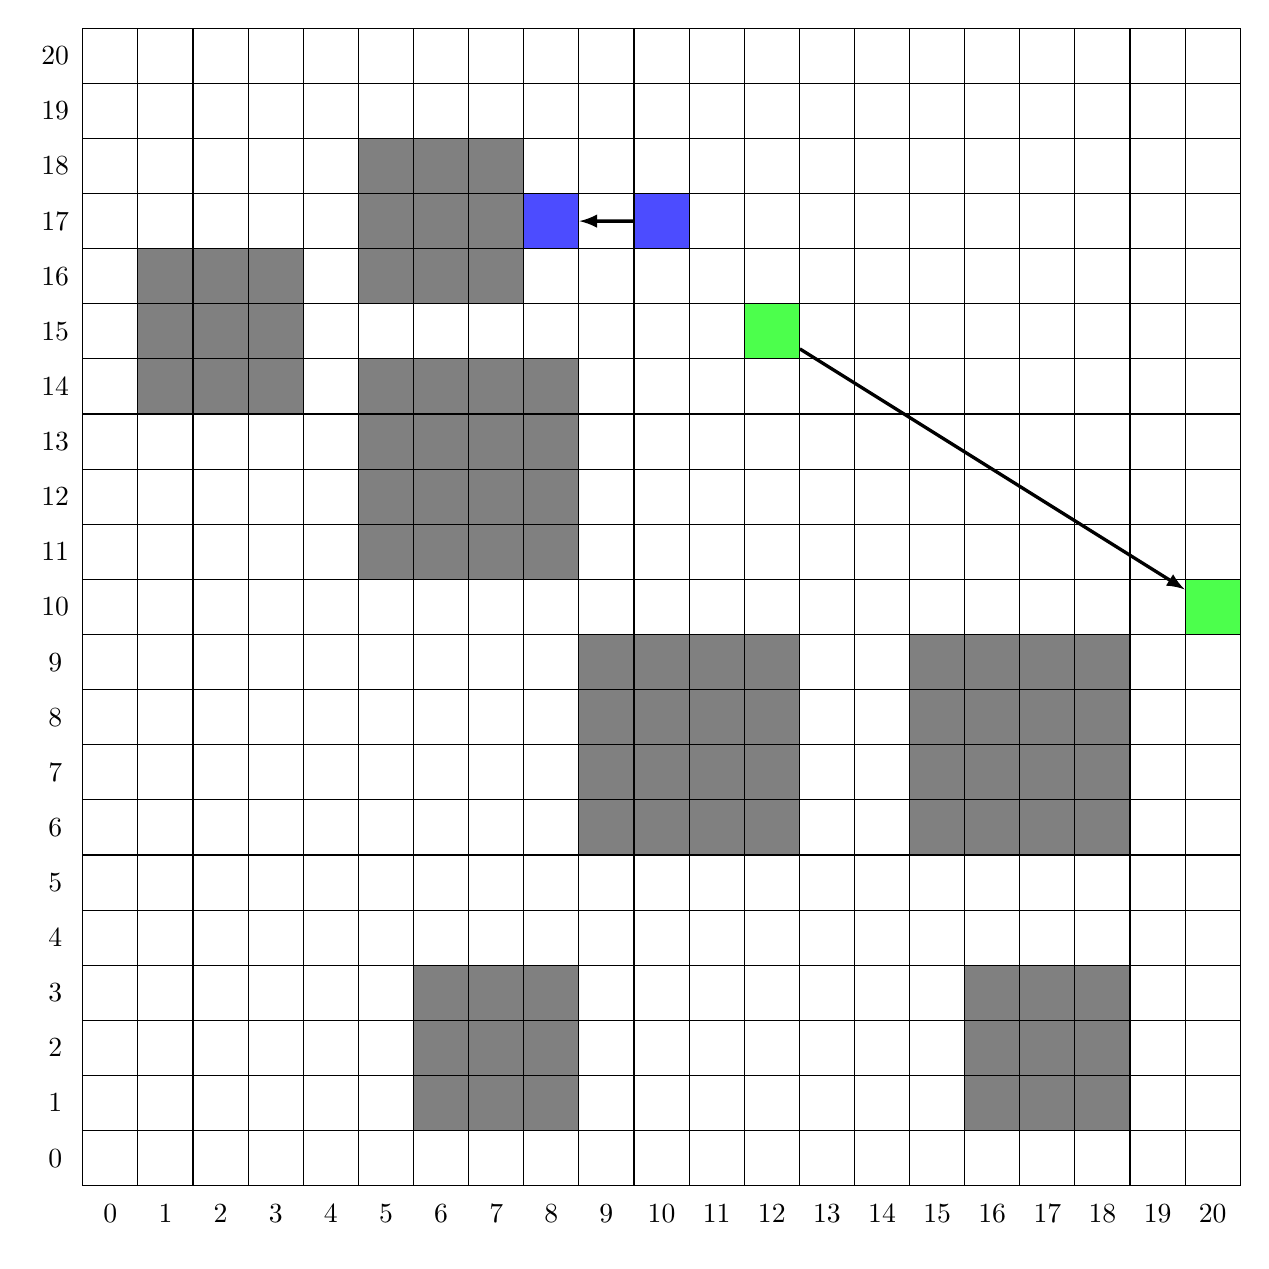
\begin{tikzpicture}[scale=\scale,
	%inner sep=1cm*\scale*\half,
	inner sep=0,
	minimum size=1cm*\scale,
	>=latex,
	pins/.style={rectangle,draw,fill=brown,font=\scriptsize},
	arrow/.style={->,very thick},
	block/.style={gray}]
	% define the row and column number
	\def \N{21}\def \M{21}
	% blockages
	\blockage{9}{6}{12}{9}
	\blockage{5}{11}{8}{14}
	\blockage{15}{6}{18}{9}
	\blockage{1}{14}{3}{16}
	\blockage{6}{1}{8}{3}
	\blockage{16}{1}{18}{3}
	\blockage{5}{16}{7}{18}
	% nets
	\drawtwopin{Dlt18_to_Dlt26}{8}{17}{Dlt18}{10}{17}{blue!70}
	\drawtwopin{W}{20}{10}{Dlt18}{12}{15}{green!70}
	\drawgrid{\N}{\M}
	\end{tikzpicture}
	\caption{DAC05\_subproblem\_27}
	\end{figure}
	\clearpage
	\begin{figure}
	\centering
	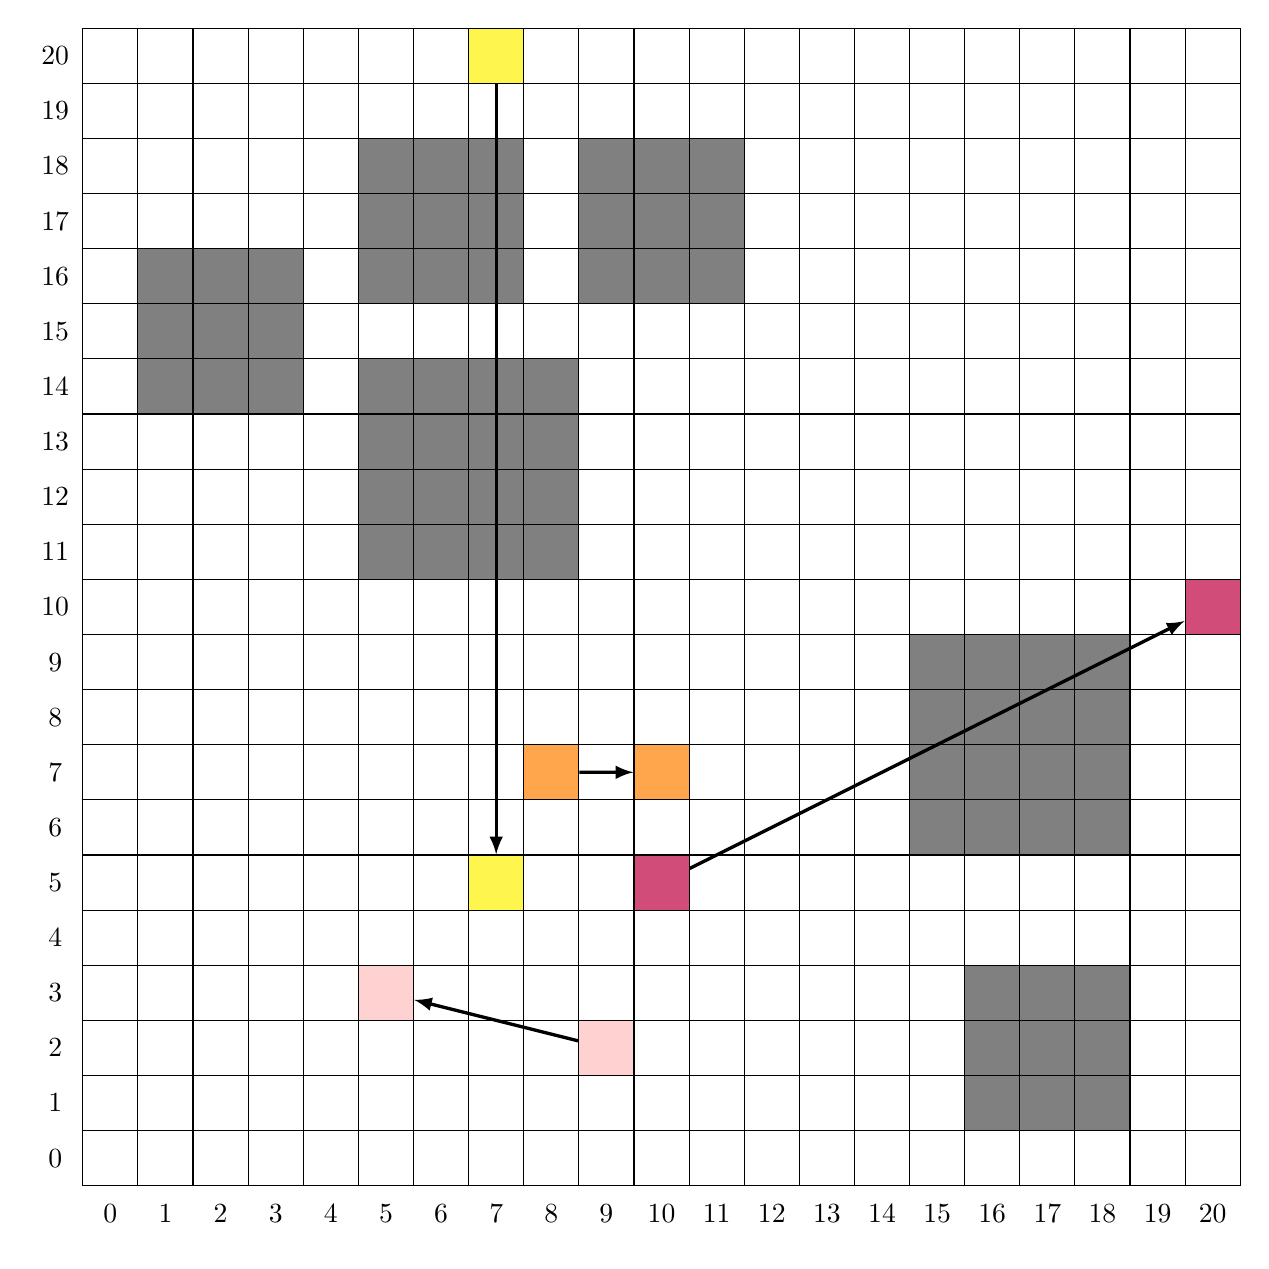
\begin{tikzpicture}[scale=\scale,
	%inner sep=1cm*\scale*\half,
	inner sep=0,
	minimum size=1cm*\scale,
	>=latex,
	pins/.style={rectangle,draw,fill=brown,font=\scriptsize},
	arrow/.style={->,very thick},
	block/.style={gray}]
	% define the row and column number
	\def \N{21}\def \M{21}
	% blockages
	\blockage{5}{11}{8}{14}
	\blockage{15}{6}{18}{9}
	\blockage{1}{14}{3}{16}
	\blockage{16}{1}{18}{3}
	\blockage{5}{16}{7}{18}
	\blockage{9}{16}{11}{18}
	% nets
	\drawtwopin{Dlt17_to_Dlt25}{10}{7}{Dlt17}{8}{7}{orange!70}
	\drawtwopin{W}{20}{10}{Dlt17}{10}{5}{purple!70}
	\drawtwopin{Dlt22}{7}{5}{B1}{7}{20}{yellow!70}
	\drawtwopin{Dlt22}{5}{3}{Dlt14_to_Dlt22}{9}{2}{pink!70}
	\drawgrid{\N}{\M}
	\end{tikzpicture}
	\caption{DAC05\_subproblem\_28}
	\end{figure}
	\clearpage
	\begin{figure}
	\centering
	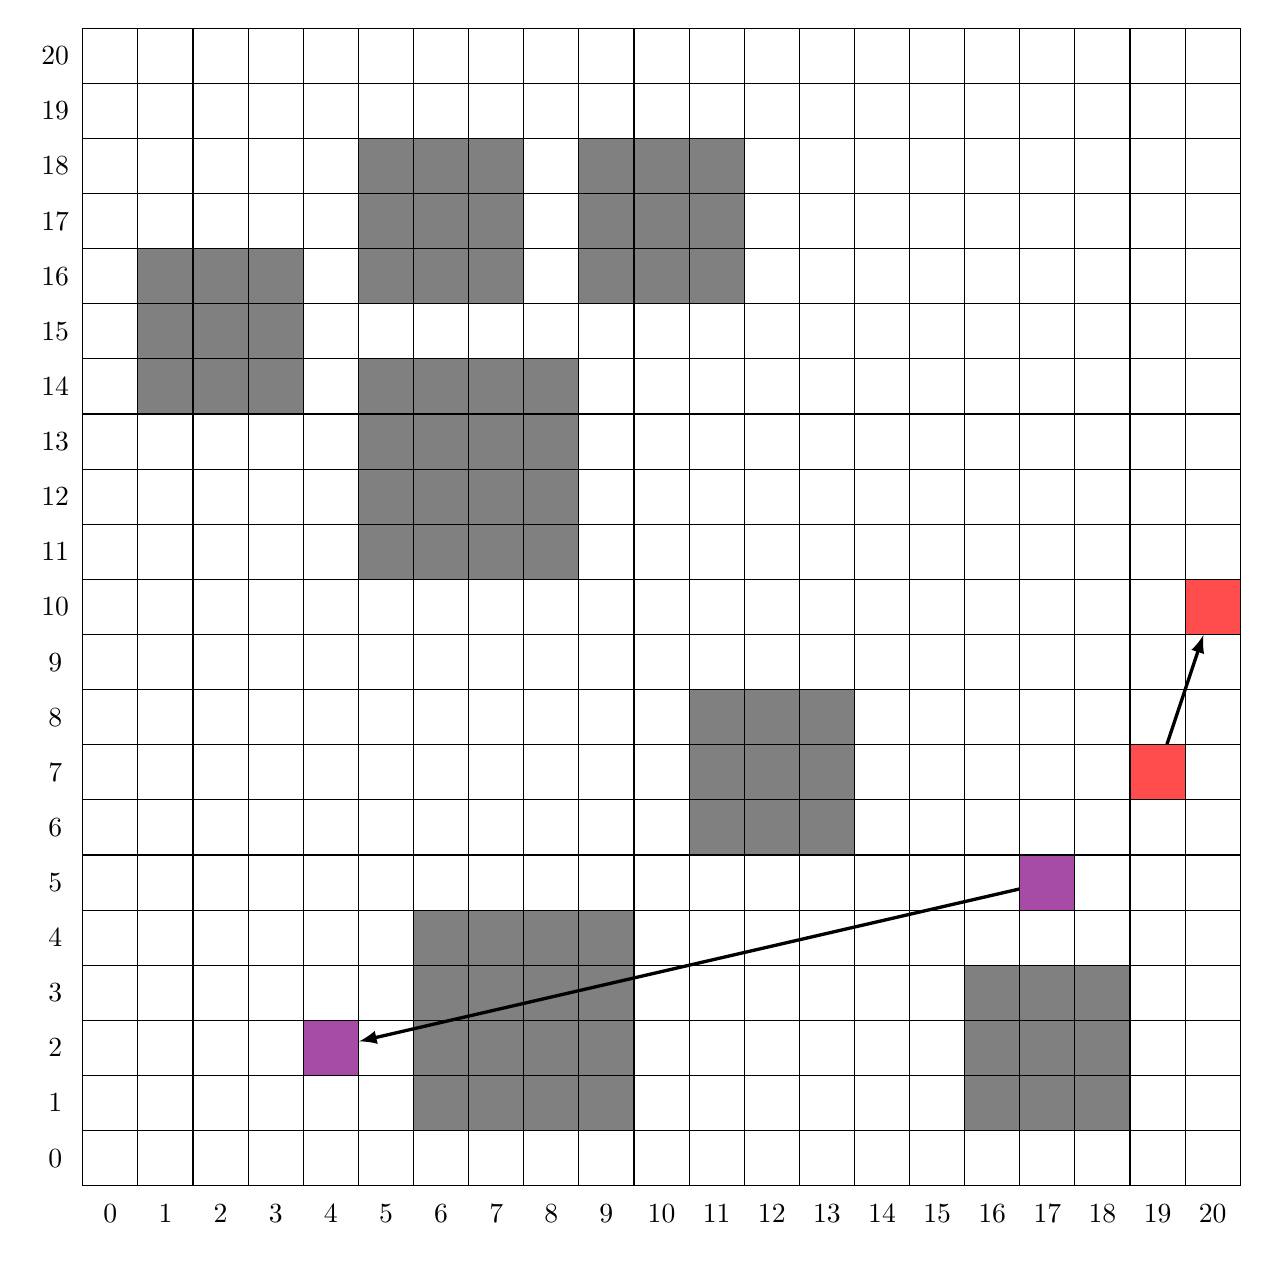
\begin{tikzpicture}[scale=\scale,
	%inner sep=1cm*\scale*\half,
	inner sep=0,
	minimum size=1cm*\scale,
	>=latex,
	pins/.style={rectangle,draw,fill=brown,font=\scriptsize},
	arrow/.style={->,very thick},
	block/.style={gray}]
	% define the row and column number
	\def \N{21}\def \M{21}
	% blockages
	\blockage{5}{11}{8}{14}
	\blockage{6}{1}{9}{4}
	\blockage{1}{14}{3}{16}
	\blockage{16}{1}{18}{3}
	\blockage{5}{16}{7}{18}
	\blockage{11}{6}{13}{8}
	\blockage{9}{16}{11}{18}
	% nets
	\drawtwopin{Dlt20_to_Dlt28}{4}{2}{Dlt20}{17}{5}{violet!70}
	\drawtwopin{W}{20}{10}{Dlt20}{19}{7}{red!70}
	\drawgrid{\N}{\M}
	\end{tikzpicture}
	\caption{DAC05\_subproblem\_29}
	\end{figure}
	\clearpage
	\begin{figure}
	\centering
	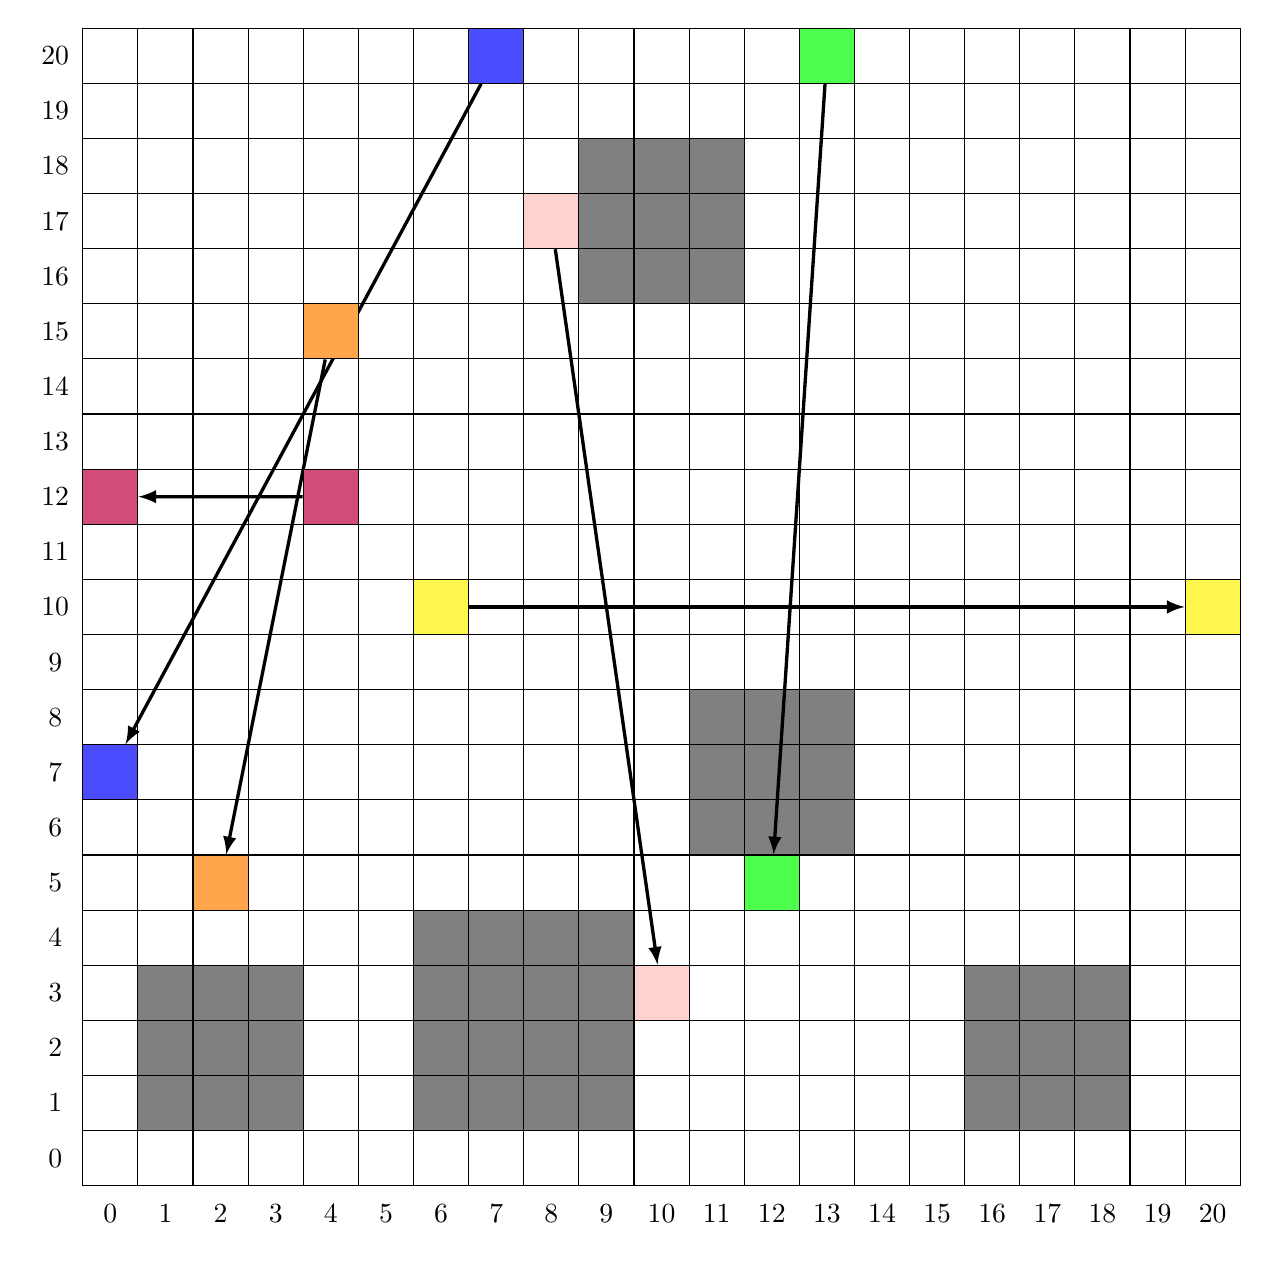
\begin{tikzpicture}[scale=\scale,
	%inner sep=1cm*\scale*\half,
	inner sep=0,
	minimum size=1cm*\scale,
	>=latex,
	pins/.style={rectangle,draw,fill=brown,font=\scriptsize},
	arrow/.style={->,very thick},
	block/.style={gray}]
	% define the row and column number
	\def \N{21}\def \M{21}
	% blockages
	\blockage{6}{1}{9}{4}
	\blockage{16}{1}{18}{3}
	\blockage{11}{6}{13}{8}
	\blockage{9}{16}{11}{18}
	\blockage{1}{1}{3}{3}
	% nets
	\drawtwopin{Dlt21}{0}{7}{B1}{7}{20}{blue!70}
	\drawtwopin{Dlt24}{12}{5}{B2}{13}{20}{green!70}
	\drawtwopin{Dlt21}{2}{5}{Dlt13_to_Dlt21}{4}{15}{orange!70}
	\drawtwopin{Dlt19_to_Dlt27}{0}{12}{Dlt19}{4}{12}{purple!70}
	\drawtwopin{W}{20}{10}{Dlt19}{6}{10}{yellow!70}
	\drawtwopin{Dlt24}{10}{3}{Dlt16_to_Dlt24}{8}{17}{pink!70}
	\drawgrid{\N}{\M}
	\end{tikzpicture}
	\caption{DAC05\_subproblem\_30}
	\end{figure}
	\clearpage
	\begin{figure}
	\centering
	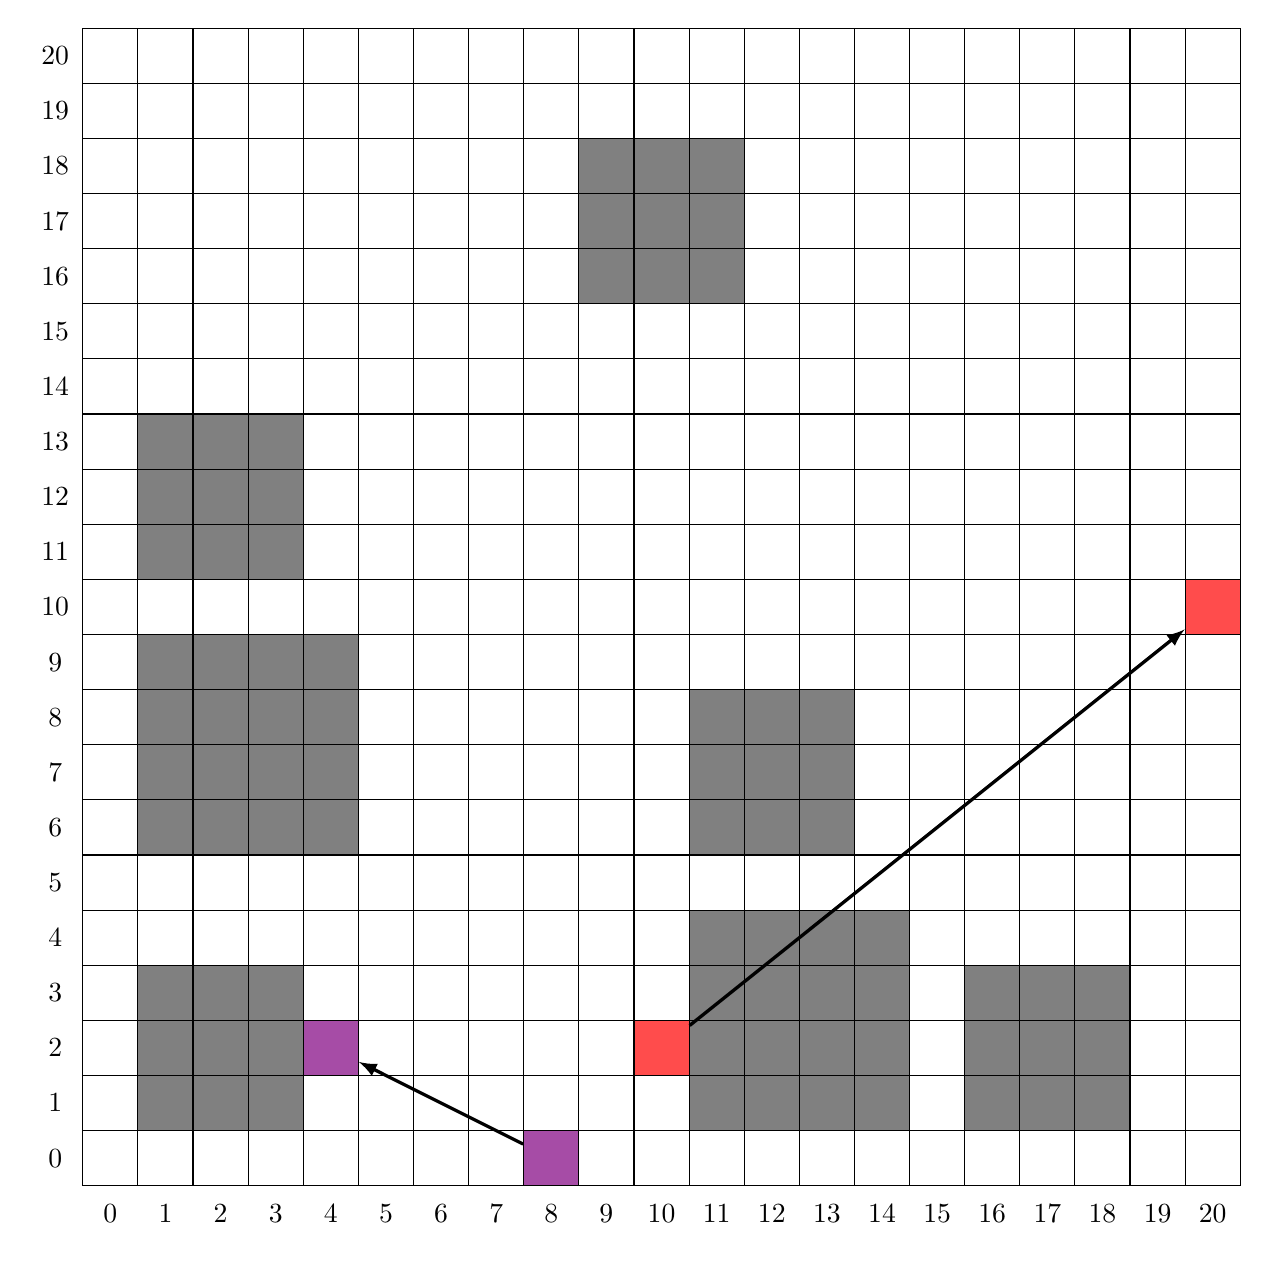
\begin{tikzpicture}[scale=\scale,
	%inner sep=1cm*\scale*\half,
	inner sep=0,
	minimum size=1cm*\scale,
	>=latex,
	pins/.style={rectangle,draw,fill=brown,font=\scriptsize},
	arrow/.style={->,very thick},
	block/.style={gray}]
	% define the row and column number
	\def \N{21}\def \M{21}
	% blockages
	\blockage{1}{6}{4}{9}
	\blockage{11}{1}{14}{4}
	\blockage{16}{1}{18}{3}
	\blockage{11}{6}{13}{8}
	\blockage{9}{16}{11}{18}
	\blockage{1}{11}{3}{13}
	\blockage{1}{1}{3}{3}
	% nets
	\drawtwopin{Dlt22_to_Dlt30}{4}{2}{Dlt22}{8}{0}{violet!70}
	\drawtwopin{W}{20}{10}{Dlt22}{10}{2}{red!70}
	\drawgrid{\N}{\M}
	\end{tikzpicture}
	\caption{DAC05\_subproblem\_31}
	\end{figure}
	\clearpage
	\begin{figure}
	\centering
	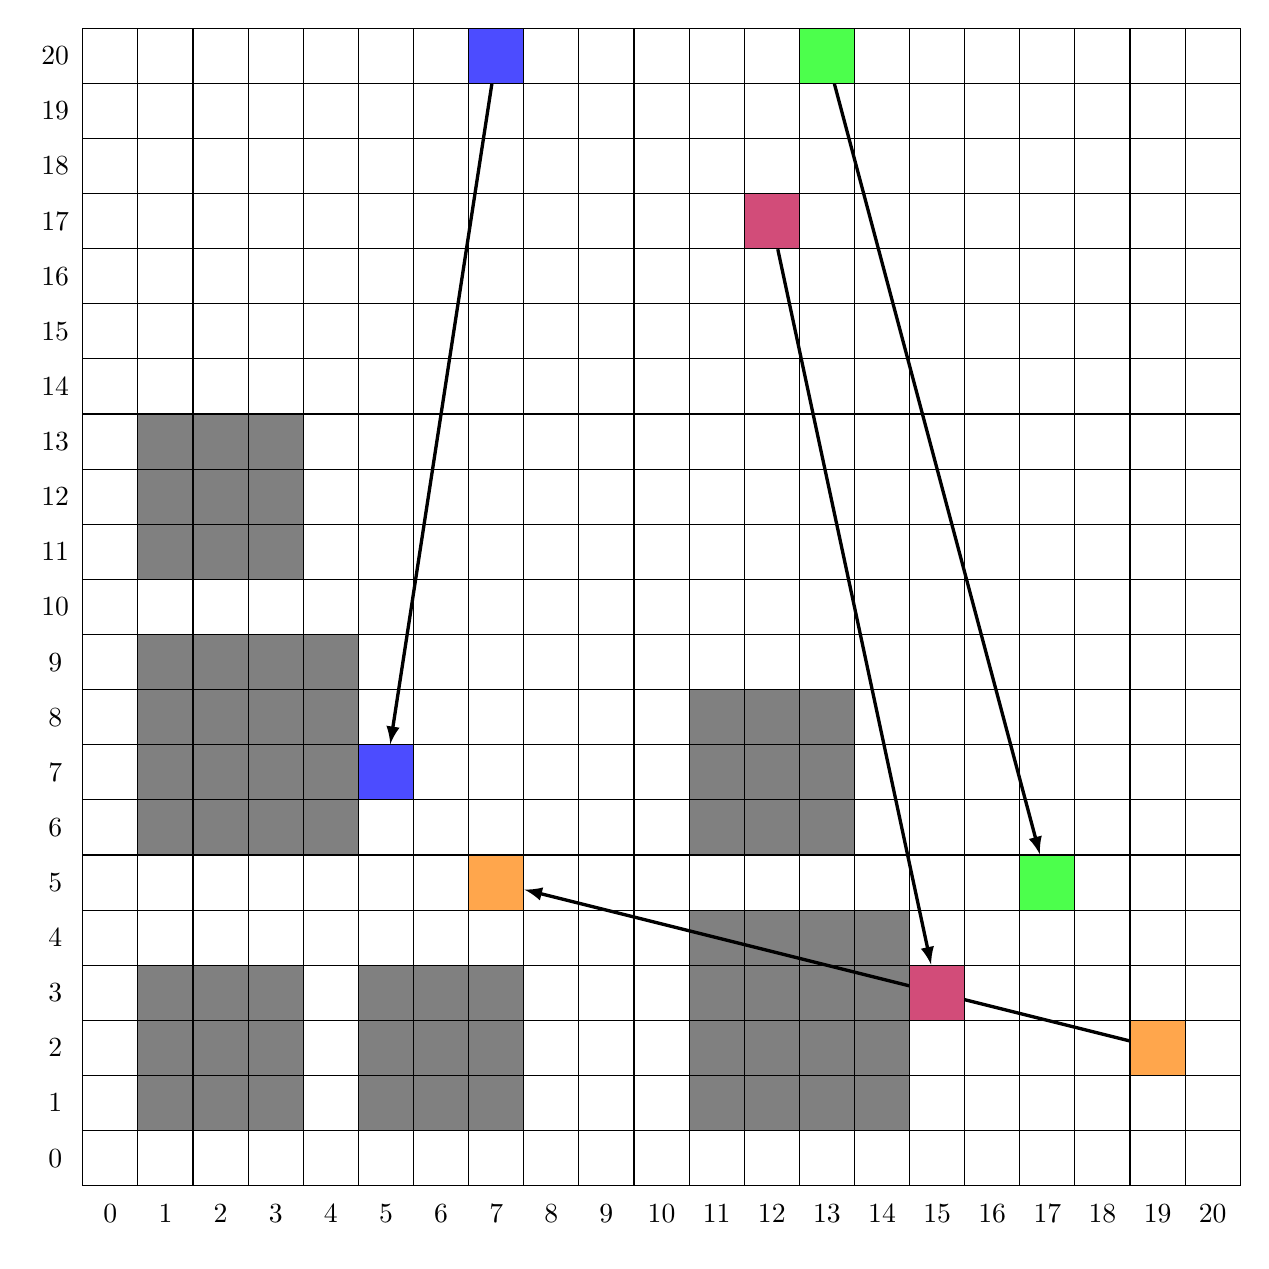
\begin{tikzpicture}[scale=\scale,
	%inner sep=1cm*\scale*\half,
	inner sep=0,
	minimum size=1cm*\scale,
	>=latex,
	pins/.style={rectangle,draw,fill=brown,font=\scriptsize},
	arrow/.style={->,very thick},
	block/.style={gray}]
	% define the row and column number
	\def \N{21}\def \M{21}
	% blockages
	\blockage{1}{6}{4}{9}
	\blockage{11}{1}{14}{4}
	\blockage{11}{6}{13}{8}
	\blockage{1}{11}{3}{13}
	\blockage{1}{1}{3}{3}
	\blockage{5}{1}{7}{3}
	% nets
	\drawtwopin{Dlt23}{5}{7}{B1}{7}{20}{blue!70}
	\drawtwopin{Dlt26}{17}{5}{B2}{13}{20}{green!70}
	\drawtwopin{Dlt23}{7}{5}{Dlt15_to_Dlt23}{19}{2}{orange!70}
	\drawtwopin{Dlt26}{15}{3}{Dlt18_to_Dlt26}{12}{17}{purple!70}
	\drawgrid{\N}{\M}
	\end{tikzpicture}
	\caption{DAC05\_subproblem\_32}
	\end{figure}
	\clearpage
	\begin{figure}
	\centering
	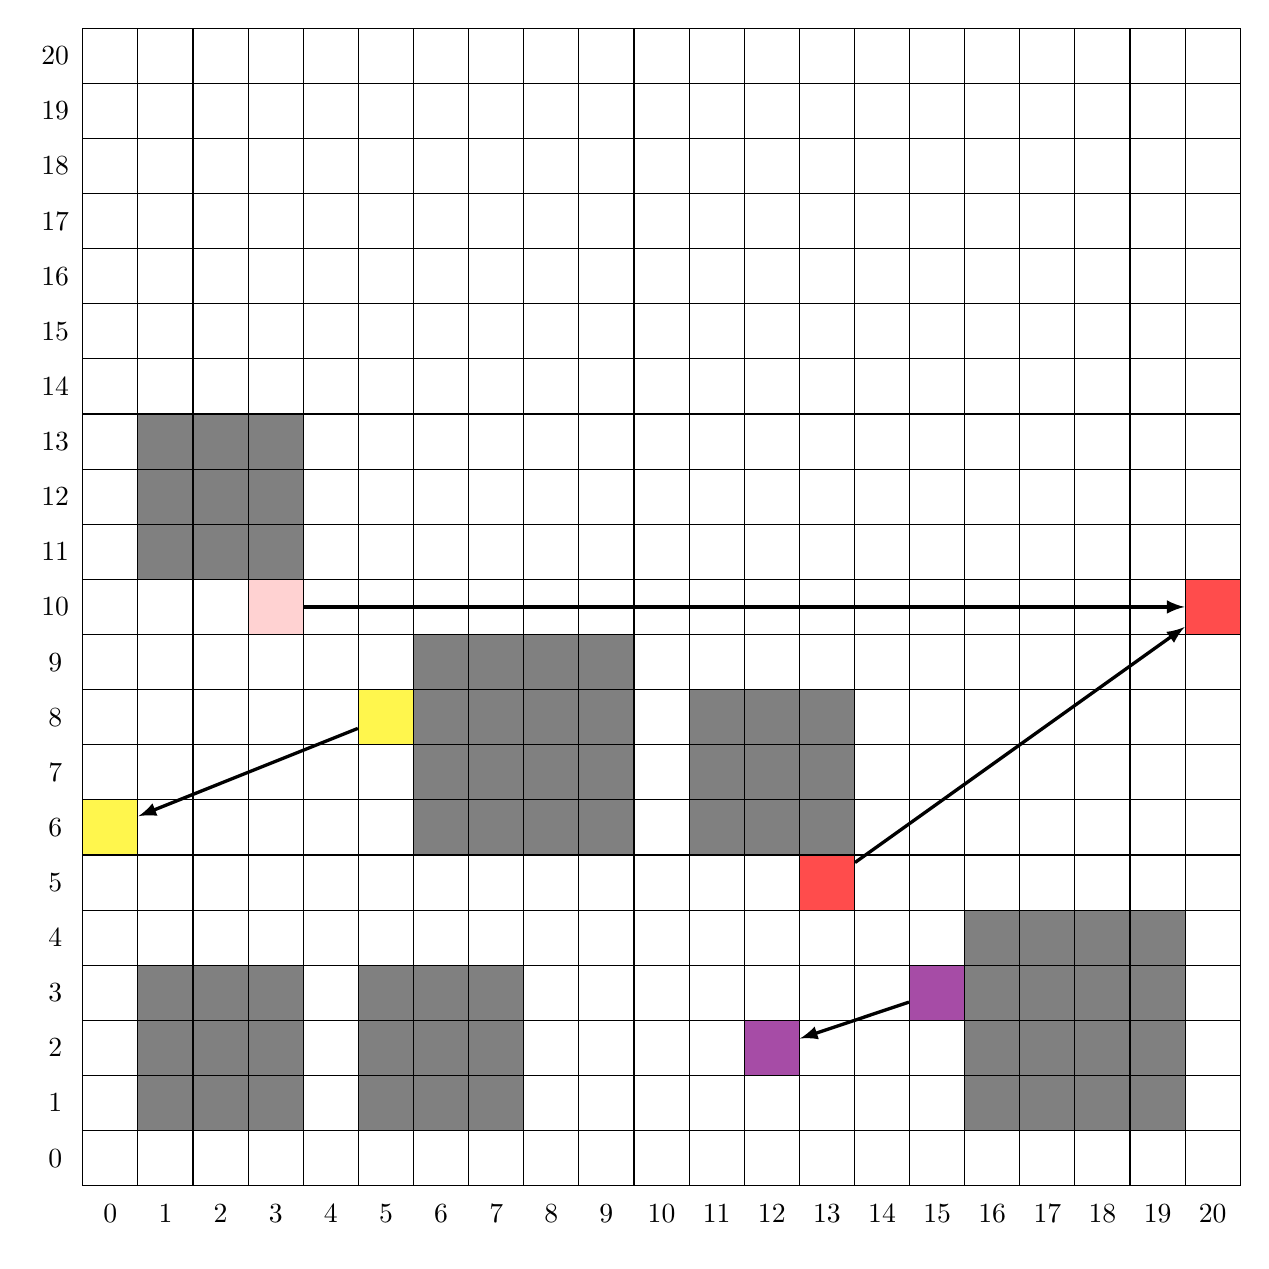
\begin{tikzpicture}[scale=\scale,
	%inner sep=1cm*\scale*\half,
	inner sep=0,
	minimum size=1cm*\scale,
	>=latex,
	pins/.style={rectangle,draw,fill=brown,font=\scriptsize},
	arrow/.style={->,very thick},
	block/.style={gray}]
	% define the row and column number
	\def \N{21}\def \M{21}
	% blockages
	\blockage{6}{6}{9}{9}
	\blockage{16}{1}{19}{4}
	\blockage{11}{6}{13}{8}
	\blockage{1}{11}{3}{13}
	\blockage{1}{1}{3}{3}
	\blockage{5}{1}{7}{3}
	% nets
	\drawtwopin{Dlt21_to_Dlt29}{0}{6}{Dlt21}{5}{8}{yellow!70}
	\drawtwopin{W}{20}{10}{Dlt21}{3}{10}{pink!70}
	\drawtwopin{Dlt24_to_Dlt32}{12}{2}{Dlt24}{15}{3}{violet!70}
	\drawtwopin{W}{20}{10}{Dlt24}{13}{5}{red!70}
	\drawgrid{\N}{\M}
	\end{tikzpicture}
	\caption{DAC05\_subproblem\_33}
	\end{figure}
	\clearpage
	\begin{figure}
	\centering
	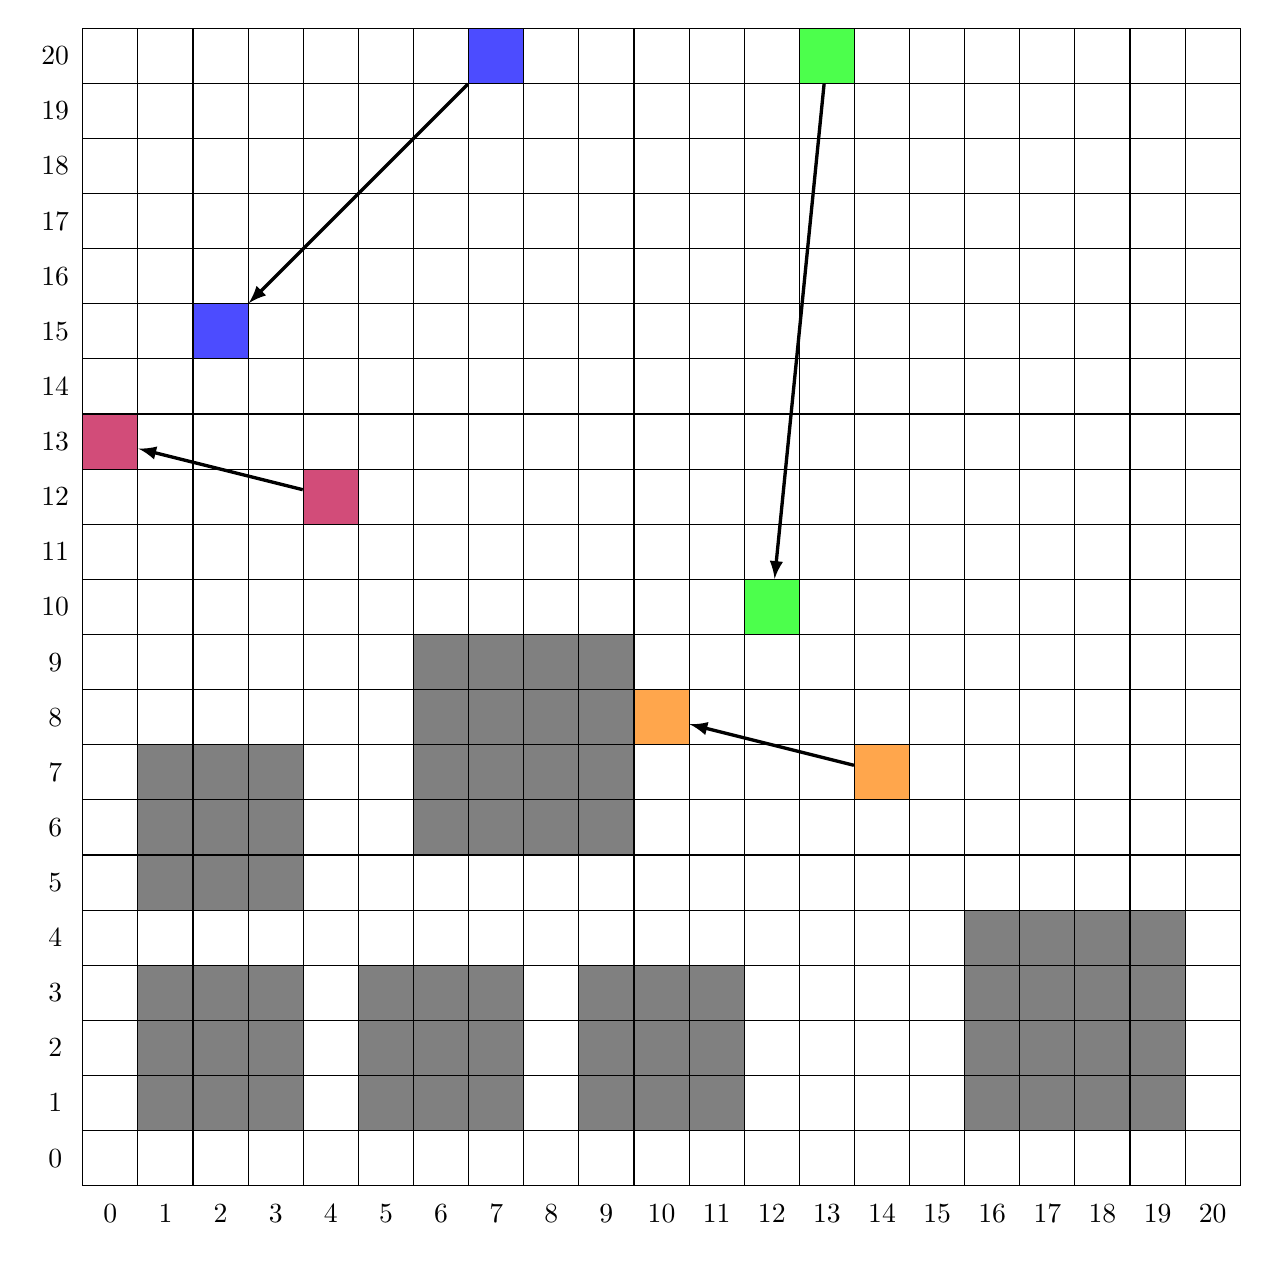
\begin{tikzpicture}[scale=\scale,
	%inner sep=1cm*\scale*\half,
	inner sep=0,
	minimum size=1cm*\scale,
	>=latex,
	pins/.style={rectangle,draw,fill=brown,font=\scriptsize},
	arrow/.style={->,very thick},
	block/.style={gray}]
	% define the row and column number
	\def \N{21}\def \M{21}
	% blockages
	\blockage{6}{6}{9}{9}
	\blockage{16}{1}{19}{4}
	\blockage{1}{1}{3}{3}
	\blockage{1}{5}{3}{7}
	\blockage{5}{1}{7}{3}
	\blockage{9}{1}{11}{3}
	% nets
	\drawtwopin{Dlt27}{2}{15}{B1}{7}{20}{blue!70}
	\drawtwopin{Dlt25}{12}{10}{B2}{13}{20}{green!70}
	\drawtwopin{Dlt25}{10}{8}{Dlt17_to_Dlt25}{14}{7}{orange!70}
	\drawtwopin{Dlt27}{0}{13}{Dlt19_to_Dlt27}{4}{12}{purple!70}
	\drawgrid{\N}{\M}
	\end{tikzpicture}
	\caption{DAC05\_subproblem\_34}
	\end{figure}
	\clearpage
	\begin{figure}
	\centering
	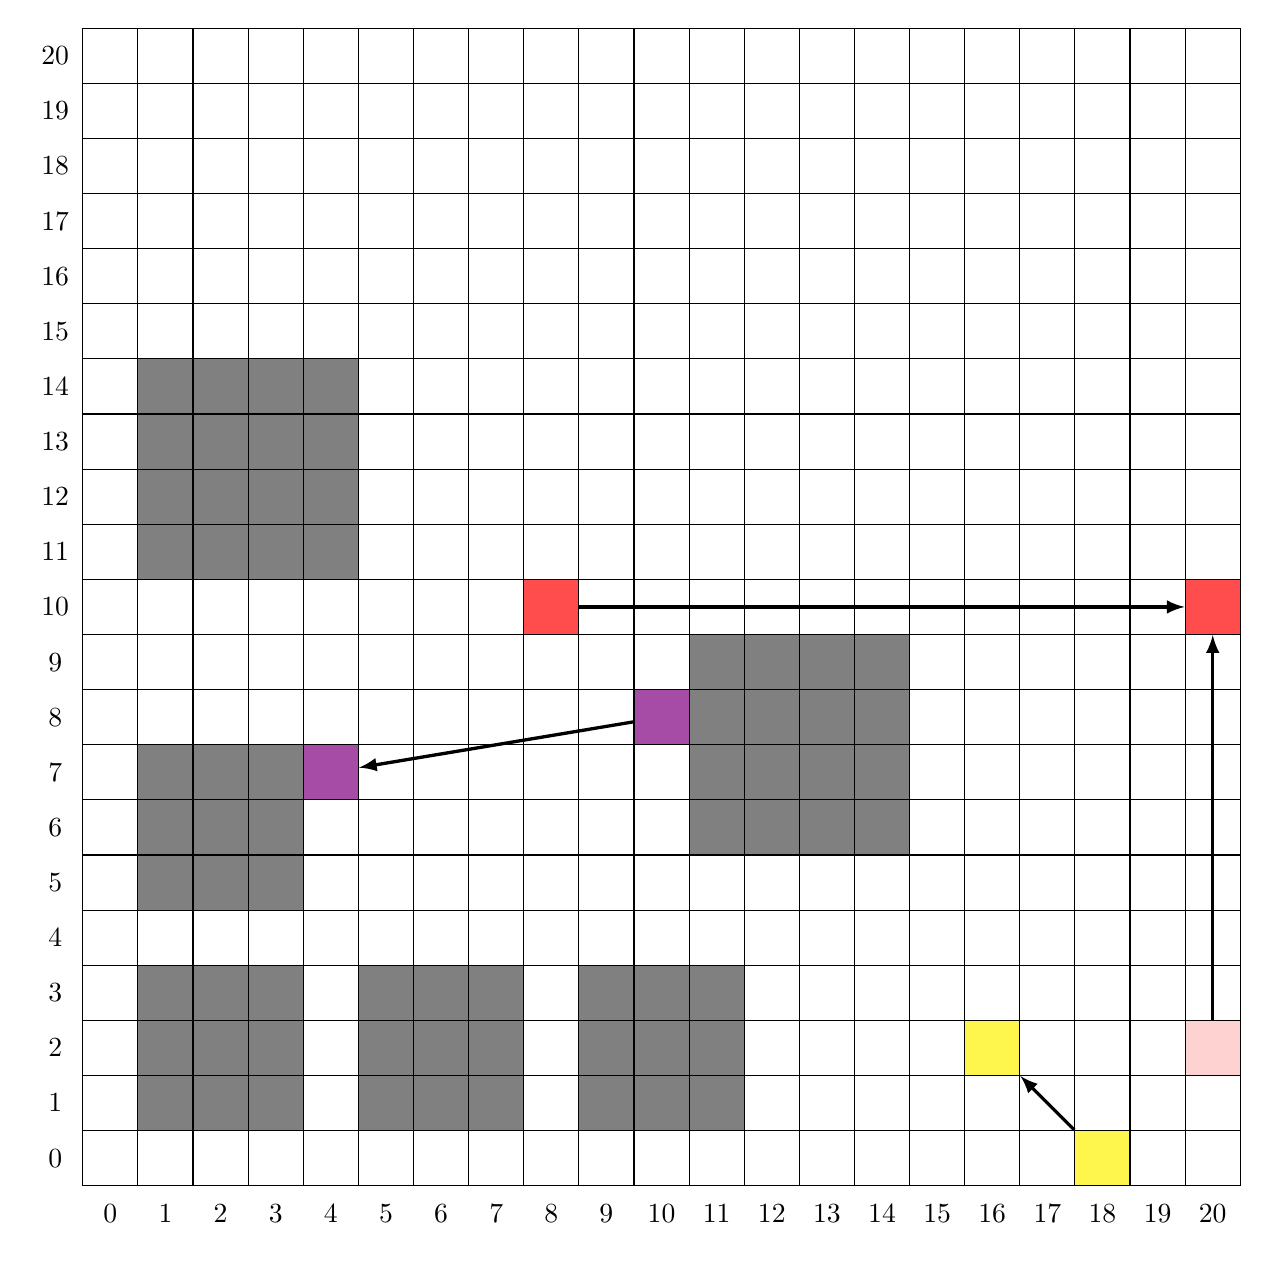
\begin{tikzpicture}[scale=\scale,
	%inner sep=1cm*\scale*\half,
	inner sep=0,
	minimum size=1cm*\scale,
	>=latex,
	pins/.style={rectangle,draw,fill=brown,font=\scriptsize},
	arrow/.style={->,very thick},
	block/.style={gray}]
	% define the row and column number
	\def \N{21}\def \M{21}
	% blockages
	\blockage{11}{6}{14}{9}
	\blockage{1}{11}{4}{14}
	\blockage{1}{1}{3}{3}
	\blockage{1}{5}{3}{7}
	\blockage{5}{1}{7}{3}
	\blockage{9}{1}{11}{3}
	% nets
	\drawtwopin{Dlt26_to_Dlt34}{16}{2}{Dlt26}{18}{0}{yellow!70}
	\drawtwopin{W}{20}{10}{Dlt26}{20}{2}{pink!70}
	\drawtwopin{Dlt23_to_Dlt31}{4}{7}{Dlt23}{10}{8}{violet!70}
	\drawtwopin{W}{20}{10}{Dlt23}{8}{10}{red!70}
	\drawgrid{\N}{\M}
	\end{tikzpicture}
	\caption{DAC05\_subproblem\_35}
	\end{figure}
	\clearpage
	\begin{figure}
	\centering
	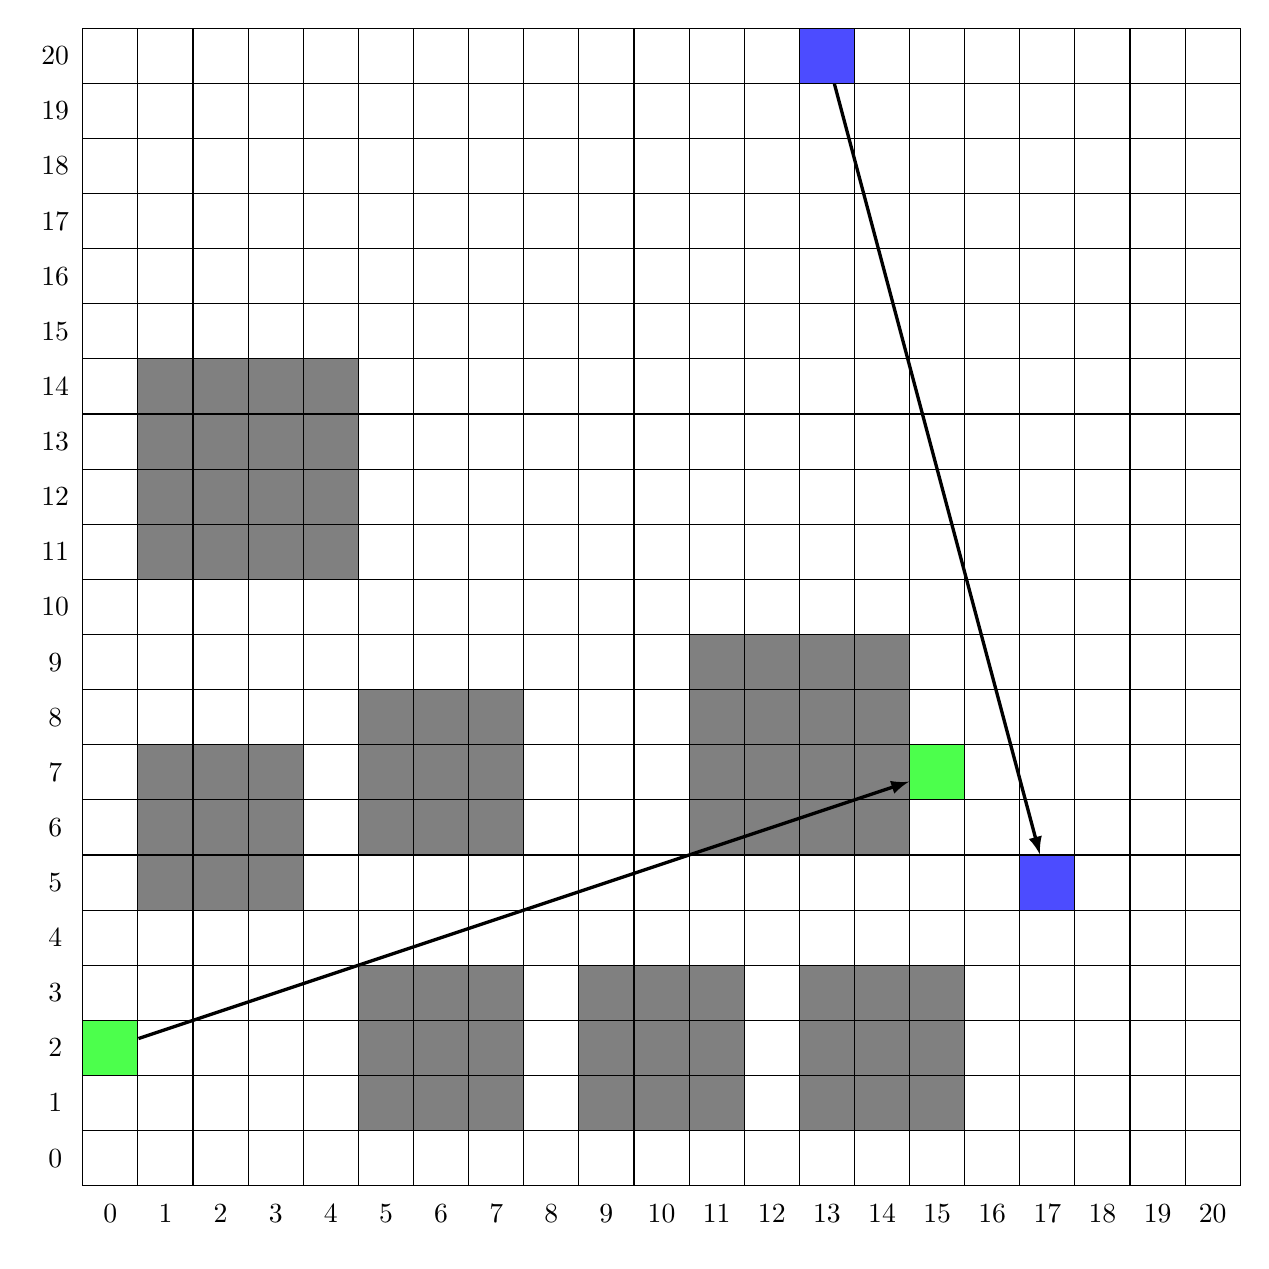
\begin{tikzpicture}[scale=\scale,
	%inner sep=1cm*\scale*\half,
	inner sep=0,
	minimum size=1cm*\scale,
	>=latex,
	pins/.style={rectangle,draw,fill=brown,font=\scriptsize},
	arrow/.style={->,very thick},
	block/.style={gray}]
	% define the row and column number
	\def \N{21}\def \M{21}
	% blockages
	\blockage{11}{6}{14}{9}
	\blockage{1}{11}{4}{14}
	\blockage{1}{5}{3}{7}
	\blockage{5}{1}{7}{3}
	\blockage{5}{6}{7}{8}
	\blockage{9}{1}{11}{3}
	\blockage{13}{1}{15}{3}
	% nets
	\drawtwopin{Dlt28}{17}{5}{B2}{13}{20}{blue!70}
	\drawtwopin{Dlt28}{15}{7}{Dlt20_to_Dlt28}{0}{2}{green!70}
	\drawgrid{\N}{\M}
	\end{tikzpicture}
	\caption{DAC05\_subproblem\_36}
	\end{figure}
	\clearpage
	\begin{figure}
	\centering
	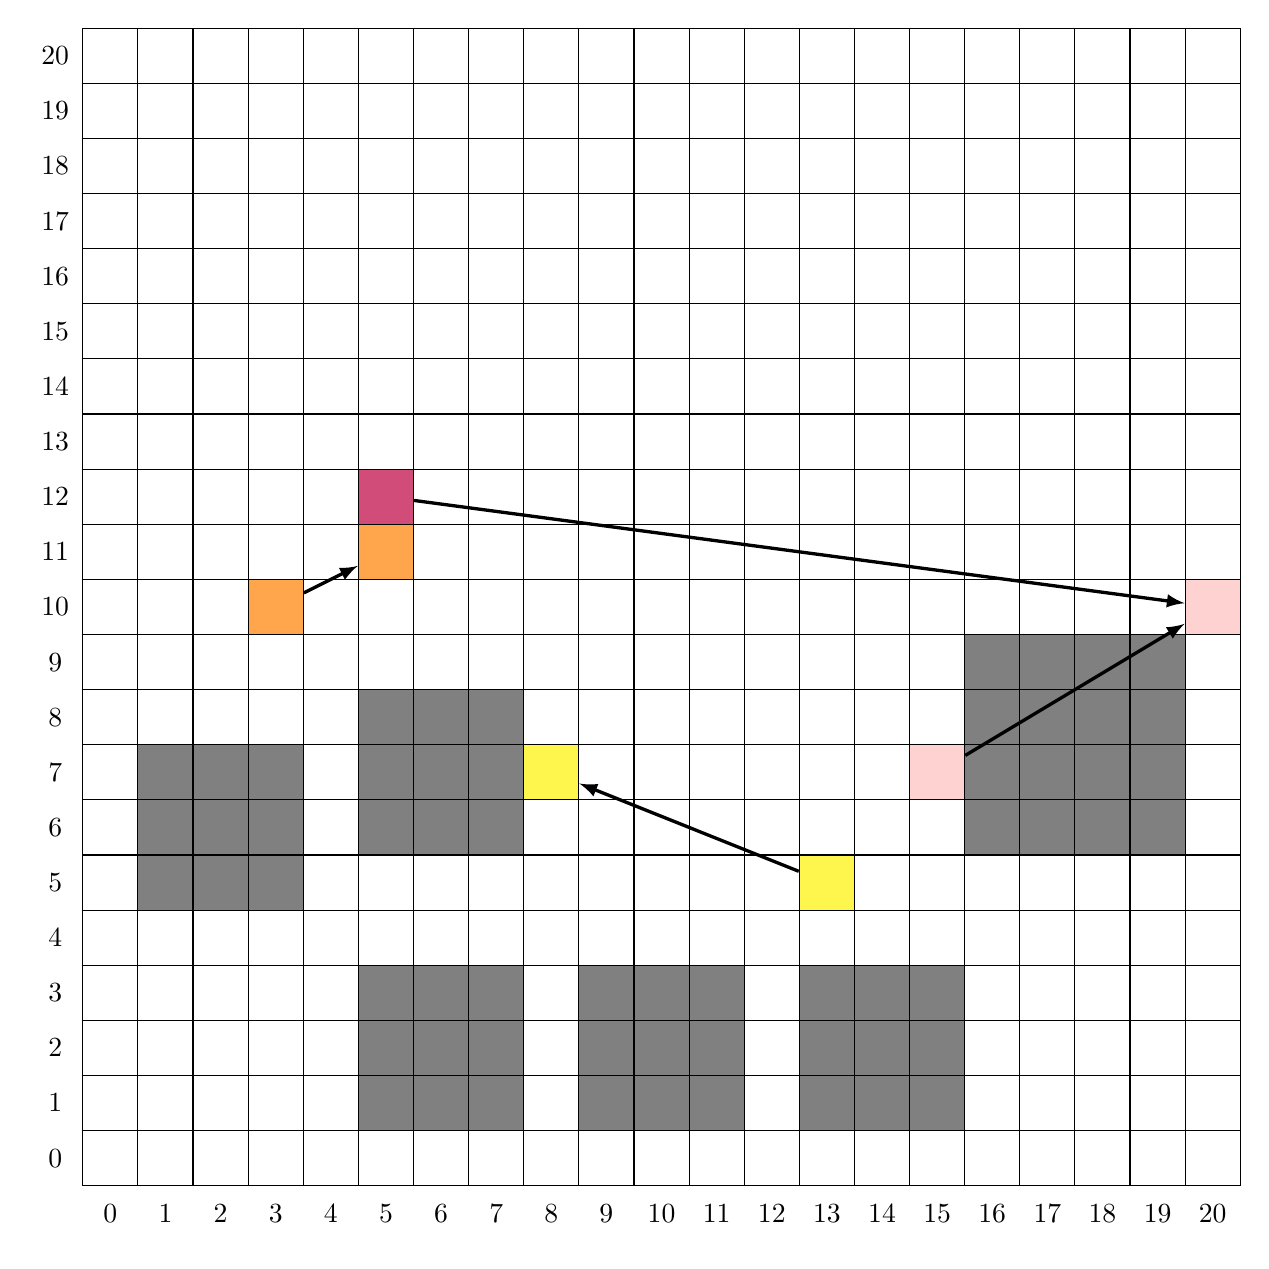
\begin{tikzpicture}[scale=\scale,
	%inner sep=1cm*\scale*\half,
	inner sep=0,
	minimum size=1cm*\scale,
	>=latex,
	pins/.style={rectangle,draw,fill=brown,font=\scriptsize},
	arrow/.style={->,very thick},
	block/.style={gray}]
	% define the row and column number
	\def \N{21}\def \M{21}
	% blockages
	\blockage{16}{6}{19}{9}
	\blockage{1}{5}{3}{7}
	\blockage{5}{1}{7}{3}
	\blockage{5}{6}{7}{8}
	\blockage{9}{1}{11}{3}
	\blockage{13}{1}{15}{3}
	% nets
	\drawtwopin{Dlt27_to_Dlt35}{5}{11}{Dlt27}{3}{10}{orange!70}
	\drawtwopin{W}{20}{10}{Dlt27}{5}{12}{purple!70}
	\drawtwopin{Dlt25_to_Dlt33}{8}{7}{Dlt25}{13}{5}{yellow!70}
	\drawtwopin{W}{20}{10}{Dlt25}{15}{7}{pink!70}
	\drawgrid{\N}{\M}
	\end{tikzpicture}
	\caption{DAC05\_subproblem\_37}
	\end{figure}
	\clearpage
	\begin{figure}
	\centering
	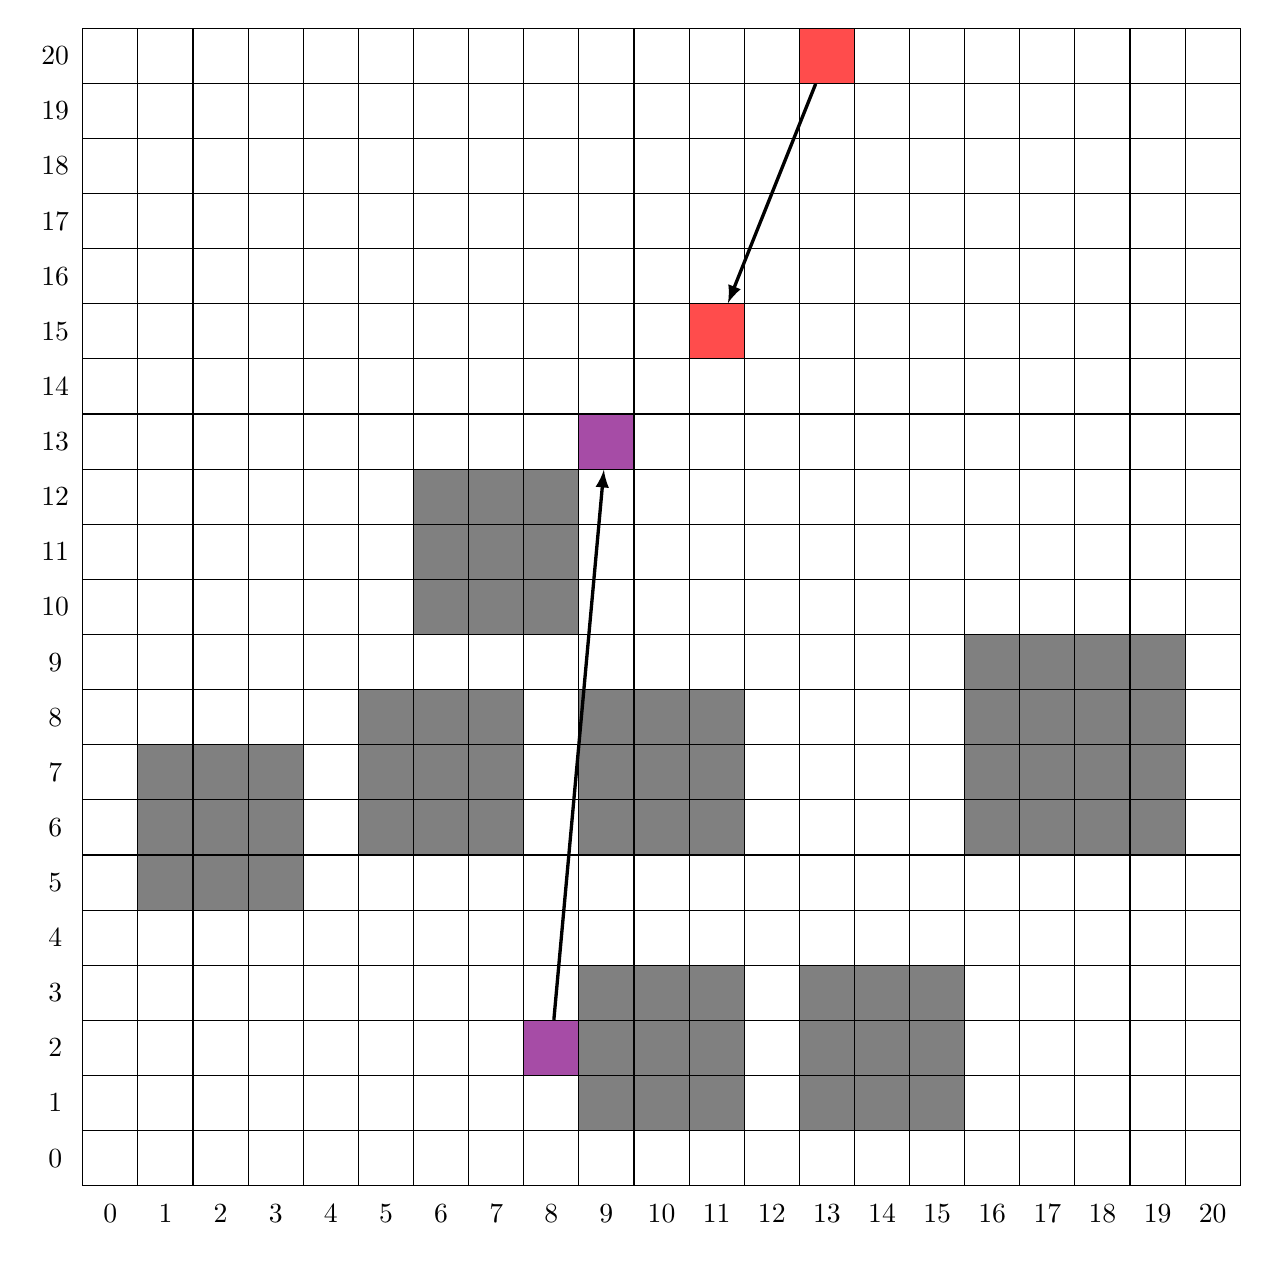
\begin{tikzpicture}[scale=\scale,
	%inner sep=1cm*\scale*\half,
	inner sep=0,
	minimum size=1cm*\scale,
	>=latex,
	pins/.style={rectangle,draw,fill=brown,font=\scriptsize},
	arrow/.style={->,very thick},
	block/.style={gray}]
	% define the row and column number
	\def \N{21}\def \M{21}
	% blockages
	\blockage{16}{6}{19}{9}
	\blockage{1}{5}{3}{7}
	\blockage{5}{6}{7}{8}
	\blockage{9}{1}{11}{3}
	\blockage{9}{6}{11}{8}
	\blockage{13}{1}{15}{3}
	\blockage{6}{10}{8}{12}
	% nets
	\drawtwopin{Dlt30}{9}{13}{Dlt22_to_Dlt30}{8}{2}{violet!70}
	\drawtwopin{Dlt30}{11}{15}{B2}{13}{20}{red!70}
	\drawgrid{\N}{\M}
	\end{tikzpicture}
	\caption{DAC05\_subproblem\_38}
	\end{figure}
	\clearpage
	\begin{figure}
	\centering
	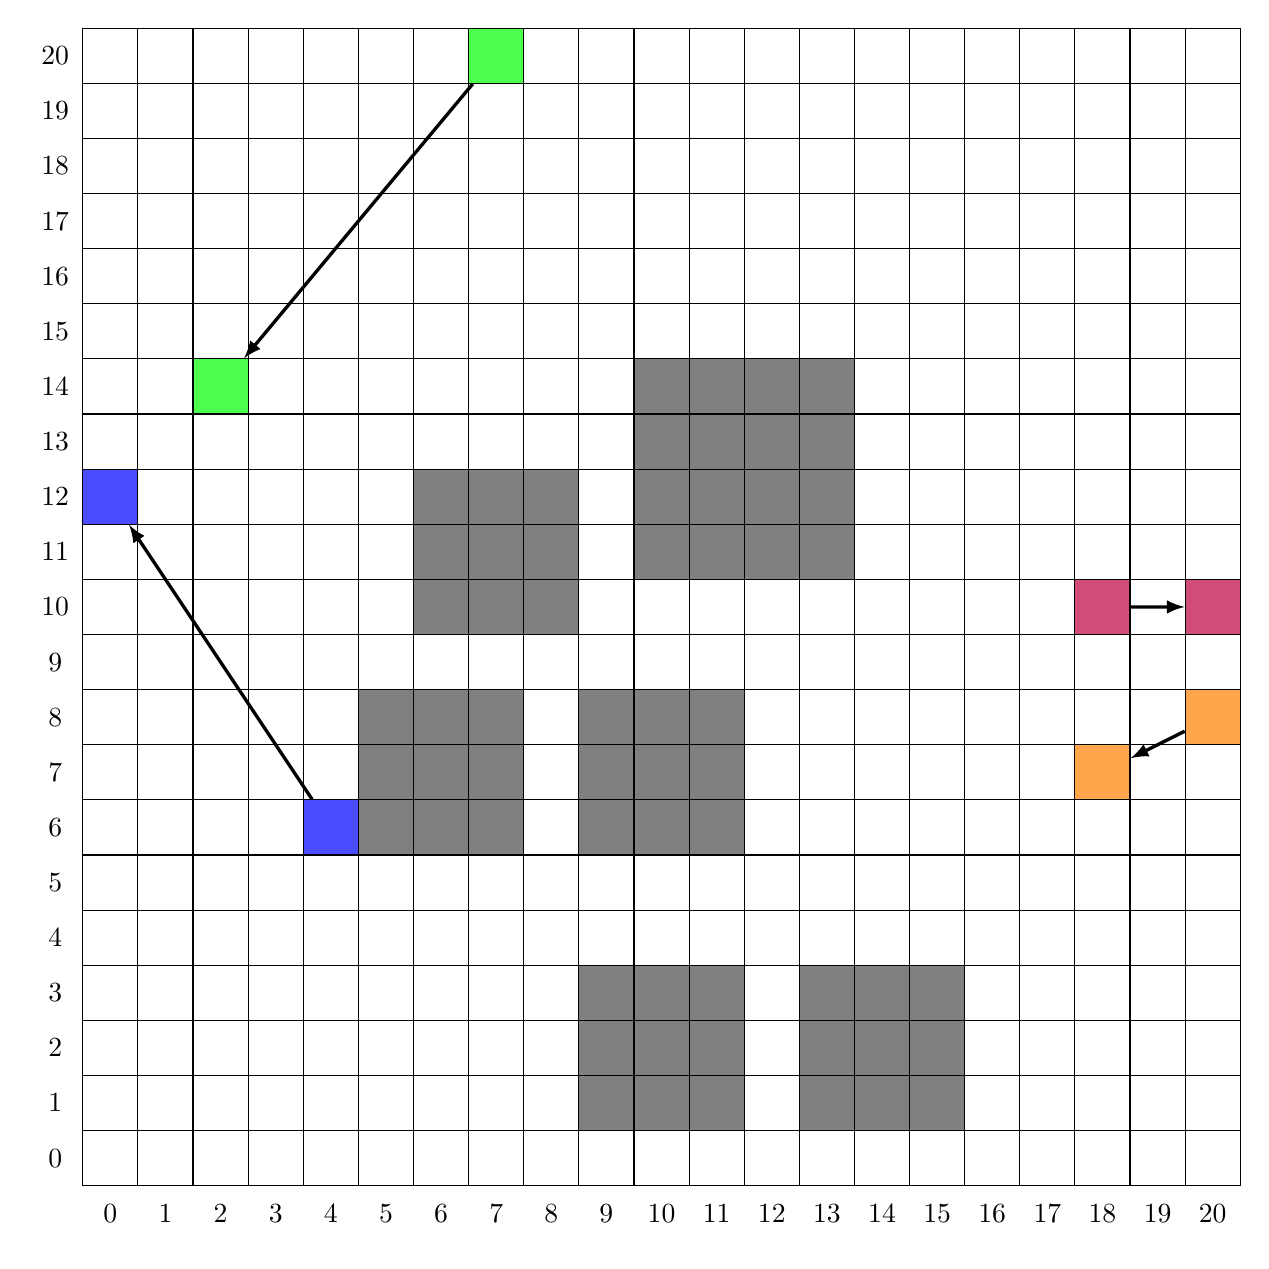
\begin{tikzpicture}[scale=\scale,
	%inner sep=1cm*\scale*\half,
	inner sep=0,
	minimum size=1cm*\scale,
	>=latex,
	pins/.style={rectangle,draw,fill=brown,font=\scriptsize},
	arrow/.style={->,very thick},
	block/.style={gray}]
	% define the row and column number
	\def \N{21}\def \M{21}
	% blockages
	\blockage{10}{11}{13}{14}
	\blockage{5}{6}{7}{8}
	\blockage{9}{1}{11}{3}
	\blockage{9}{6}{11}{8}
	\blockage{13}{1}{15}{3}
	\blockage{6}{10}{8}{12}
	% nets
	\drawtwopin{Dlt29}{0}{12}{Dlt21_to_Dlt29}{4}{6}{blue!70}
	\drawtwopin{Dlt29}{2}{14}{B1}{7}{20}{green!70}
	\drawtwopin{Dlt28_to_Dlt36}{18}{7}{Dlt28}{20}{8}{orange!70}
	\drawtwopin{W}{20}{10}{Dlt28}{18}{10}{purple!70}
	\drawgrid{\N}{\M}
	\end{tikzpicture}
	\caption{DAC05\_subproblem\_39}
	\end{figure}
	\clearpage
	\begin{figure}
	\centering
	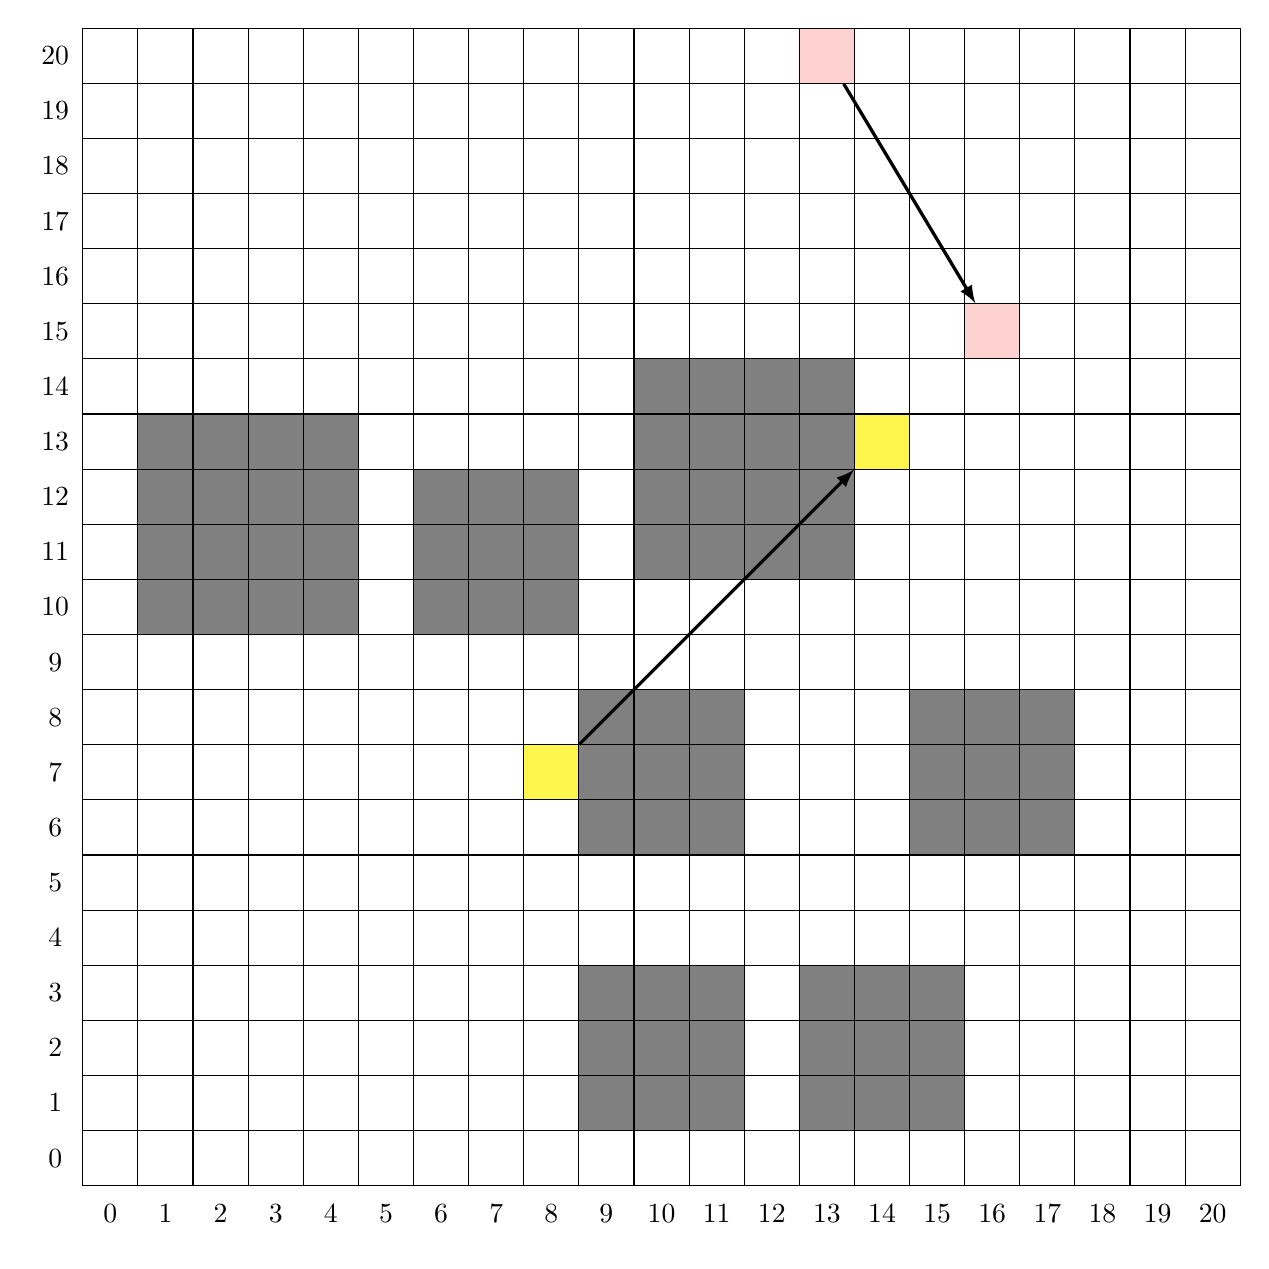
\begin{tikzpicture}[scale=\scale,
	%inner sep=1cm*\scale*\half,
	inner sep=0,
	minimum size=1cm*\scale,
	>=latex,
	pins/.style={rectangle,draw,fill=brown,font=\scriptsize},
	arrow/.style={->,very thick},
	block/.style={gray}]
	% define the row and column number
	\def \N{21}\def \M{21}
	% blockages
	\blockage{1}{10}{4}{13}
	\blockage{10}{11}{13}{14}
	\blockage{9}{1}{11}{3}
	\blockage{9}{6}{11}{8}
	\blockage{13}{1}{15}{3}
	\blockage{6}{10}{8}{12}
	\blockage{15}{6}{17}{8}
	% nets
	\drawtwopin{Dlt31}{14}{13}{Dlt23_to_Dlt31}{8}{7}{yellow!70}
	\drawtwopin{Dlt31}{16}{15}{B2}{13}{20}{pink!70}
	\drawgrid{\N}{\M}
	\end{tikzpicture}
	\caption{DAC05\_subproblem\_40}
	\end{figure}
	\clearpage
	\begin{figure}
	\centering
	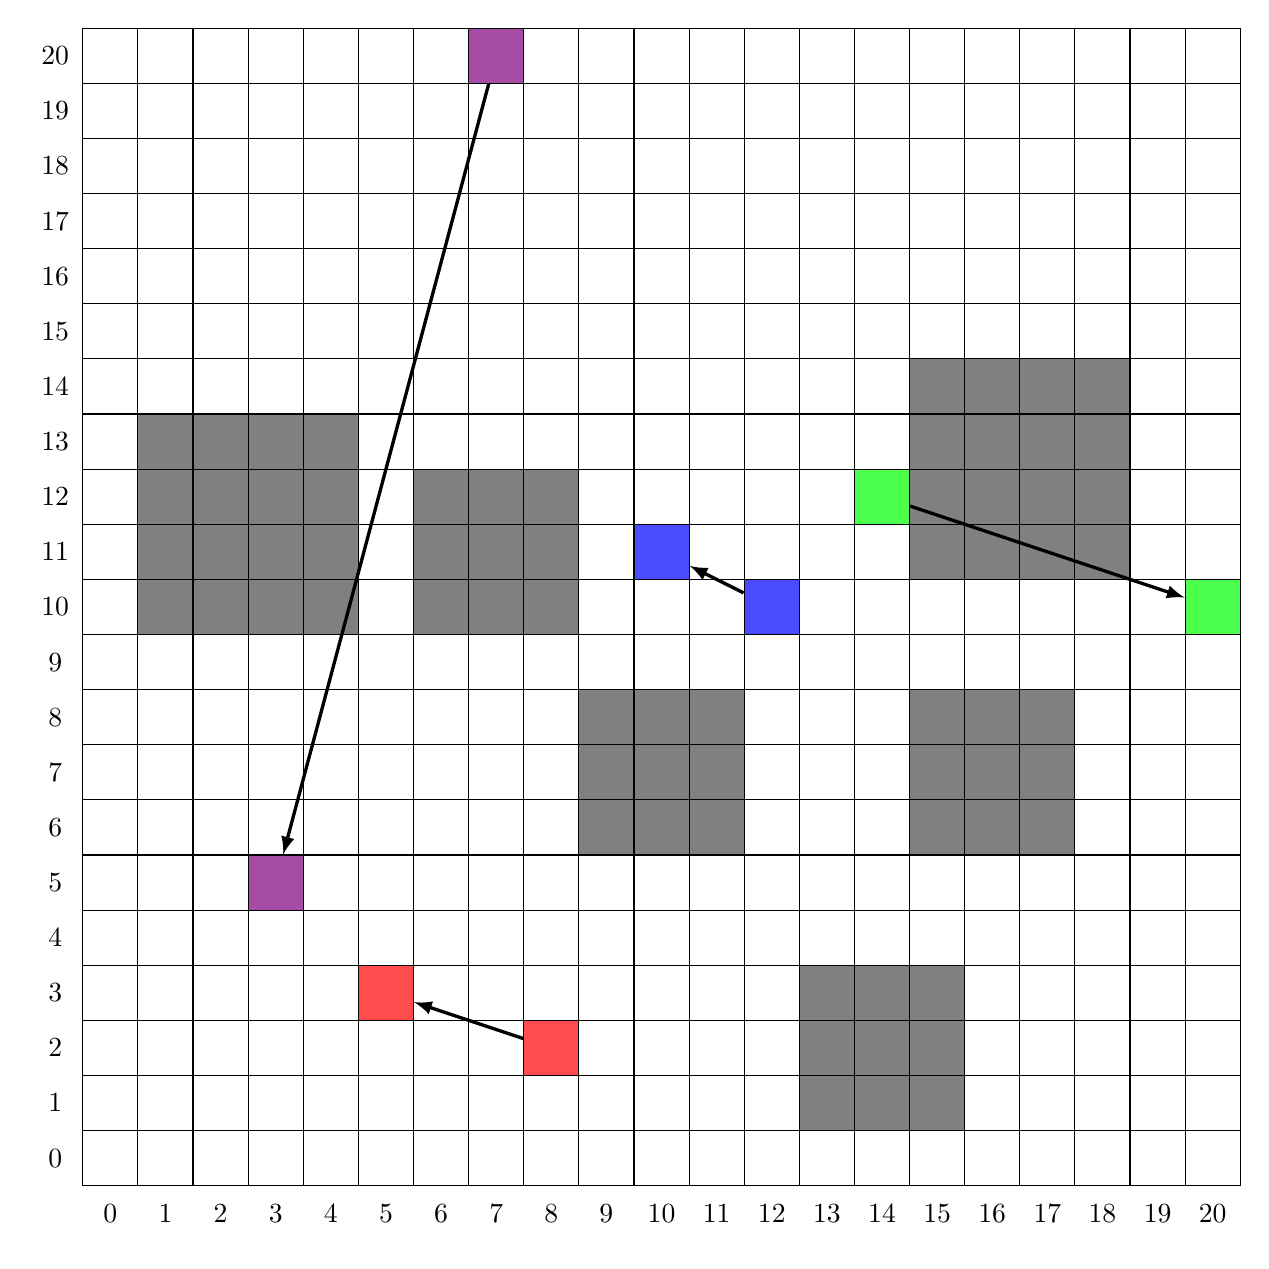
\begin{tikzpicture}[scale=\scale,
	%inner sep=1cm*\scale*\half,
	inner sep=0,
	minimum size=1cm*\scale,
	>=latex,
	pins/.style={rectangle,draw,fill=brown,font=\scriptsize},
	arrow/.style={->,very thick},
	block/.style={gray}]
	% define the row and column number
	\def \N{21}\def \M{21}
	% blockages
	\blockage{1}{10}{4}{13}
	\blockage{15}{11}{18}{14}
	\blockage{9}{6}{11}{8}
	\blockage{13}{1}{15}{3}
	\blockage{6}{10}{8}{12}
	\blockage{15}{6}{17}{8}
	% nets
	\drawtwopin{Dlt32}{3}{5}{B1}{7}{20}{violet!70}
	\drawtwopin{Dlt32}{5}{3}{Dlt24_to_Dlt32}{8}{2}{red!70}
	\drawtwopin{Dlt30_to_Dlt38}{10}{11}{Dlt30}{12}{10}{blue!70}
	\drawtwopin{W}{20}{10}{Dlt30}{14}{12}{green!70}
	\drawgrid{\N}{\M}
	\end{tikzpicture}
	\caption{DAC05\_subproblem\_41}
	\end{figure}
	\clearpage
	\begin{figure}
	\centering
	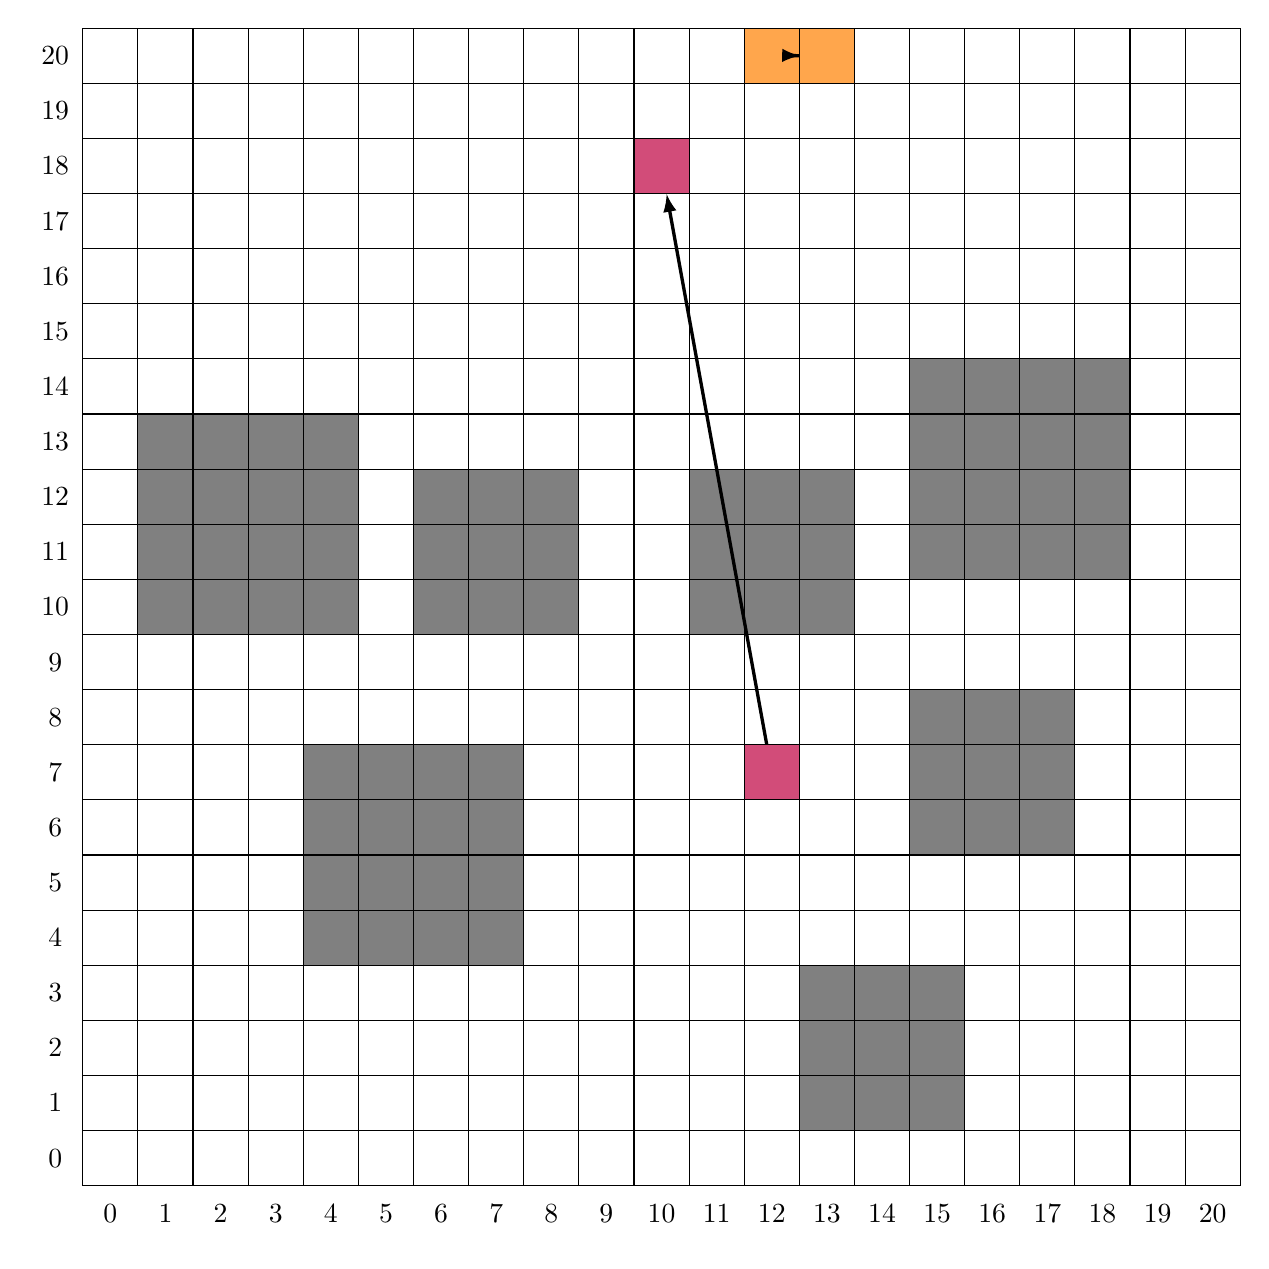
\begin{tikzpicture}[scale=\scale,
	%inner sep=1cm*\scale*\half,
	inner sep=0,
	minimum size=1cm*\scale,
	>=latex,
	pins/.style={rectangle,draw,fill=brown,font=\scriptsize},
	arrow/.style={->,very thick},
	block/.style={gray}]
	% define the row and column number
	\def \N{21}\def \M{21}
	% blockages
	\blockage{1}{10}{4}{13}
	\blockage{15}{11}{18}{14}
	\blockage{4}{4}{7}{7}
	\blockage{13}{1}{15}{3}
	\blockage{6}{10}{8}{12}
	\blockage{15}{6}{17}{8}
	\blockage{11}{10}{13}{12}
	% nets
	\drawtwopin{Dlt33}{12}{20}{B2}{13}{20}{orange!70}
	\drawtwopin{Dlt33}{10}{18}{Dlt25_to_Dlt33}{12}{7}{purple!70}
	\drawgrid{\N}{\M}
	\end{tikzpicture}
	\caption{DAC05\_subproblem\_42}
	\end{figure}
	\clearpage
	\begin{figure}
	\centering
	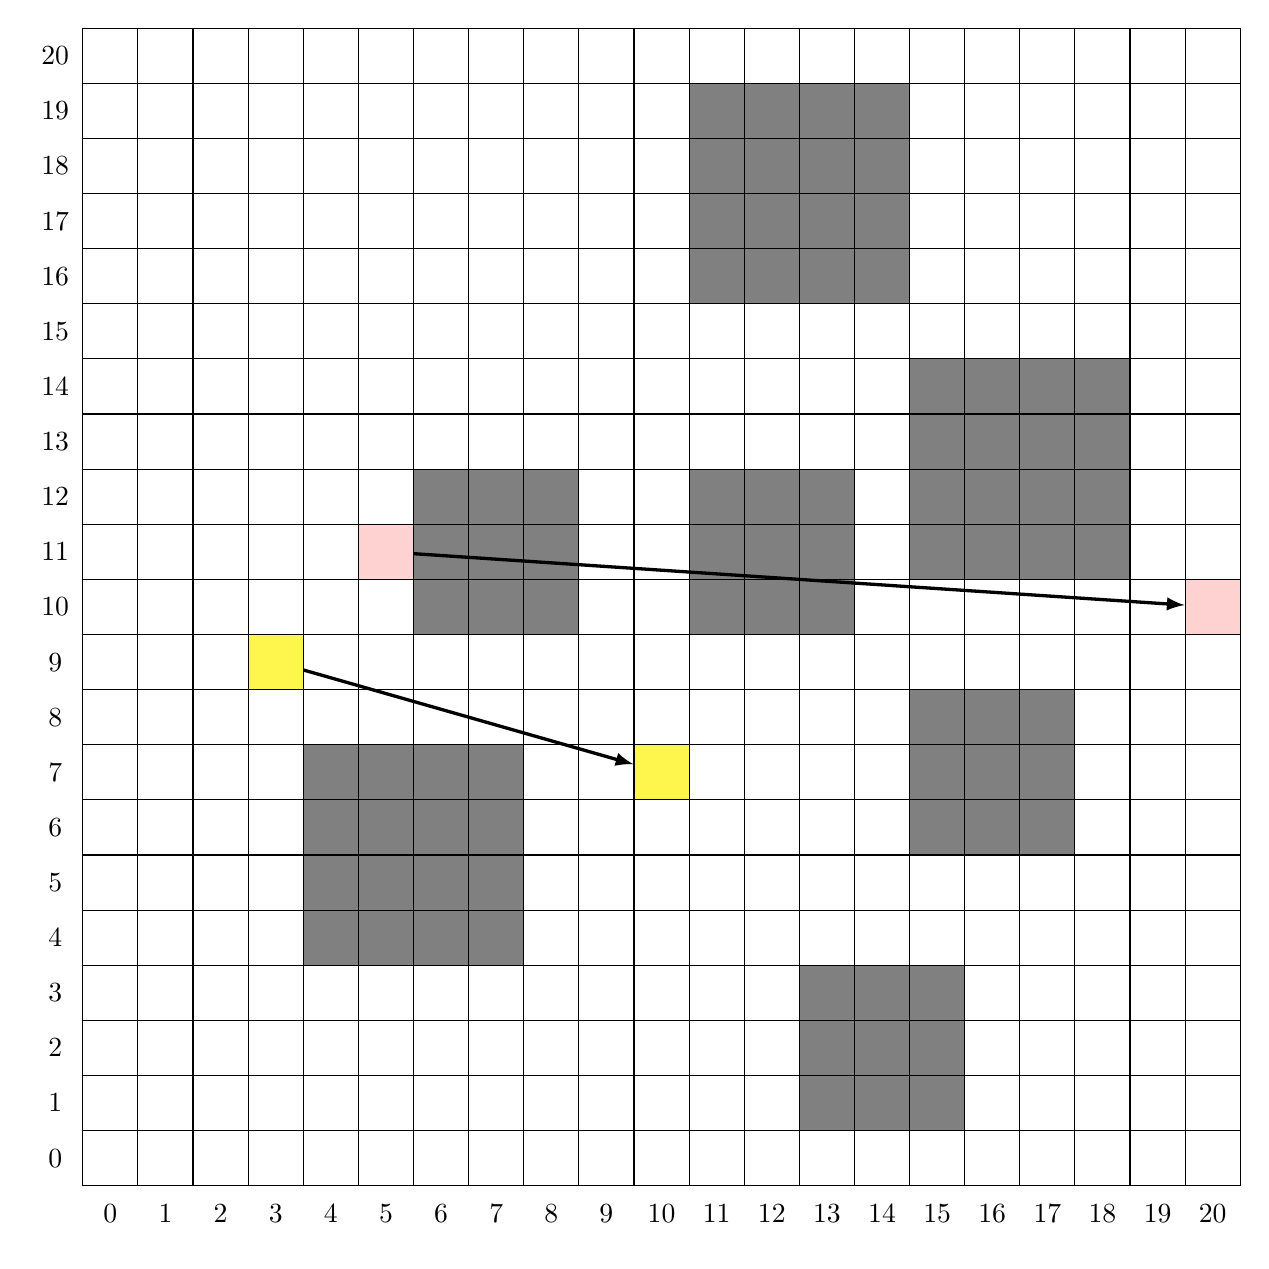
\begin{tikzpicture}[scale=\scale,
	%inner sep=1cm*\scale*\half,
	inner sep=0,
	minimum size=1cm*\scale,
	>=latex,
	pins/.style={rectangle,draw,fill=brown,font=\scriptsize},
	arrow/.style={->,very thick},
	block/.style={gray}]
	% define the row and column number
	\def \N{21}\def \M{21}
	% blockages
	\blockage{15}{11}{18}{14}
	\blockage{4}{4}{7}{7}
	\blockage{11}{16}{14}{19}
	\blockage{13}{1}{15}{3}
	\blockage{6}{10}{8}{12}
	\blockage{15}{6}{17}{8}
	\blockage{11}{10}{13}{12}
	% nets
	\drawtwopin{Dlt29_to_Dlt37}{10}{7}{Dlt29}{3}{9}{yellow!70}
	\drawtwopin{W}{20}{10}{Dlt29}{5}{11}{pink!70}
	\drawgrid{\N}{\M}
	\end{tikzpicture}
	\caption{DAC05\_subproblem\_43}
	\end{figure}
	\clearpage
	\begin{figure}
	\centering
	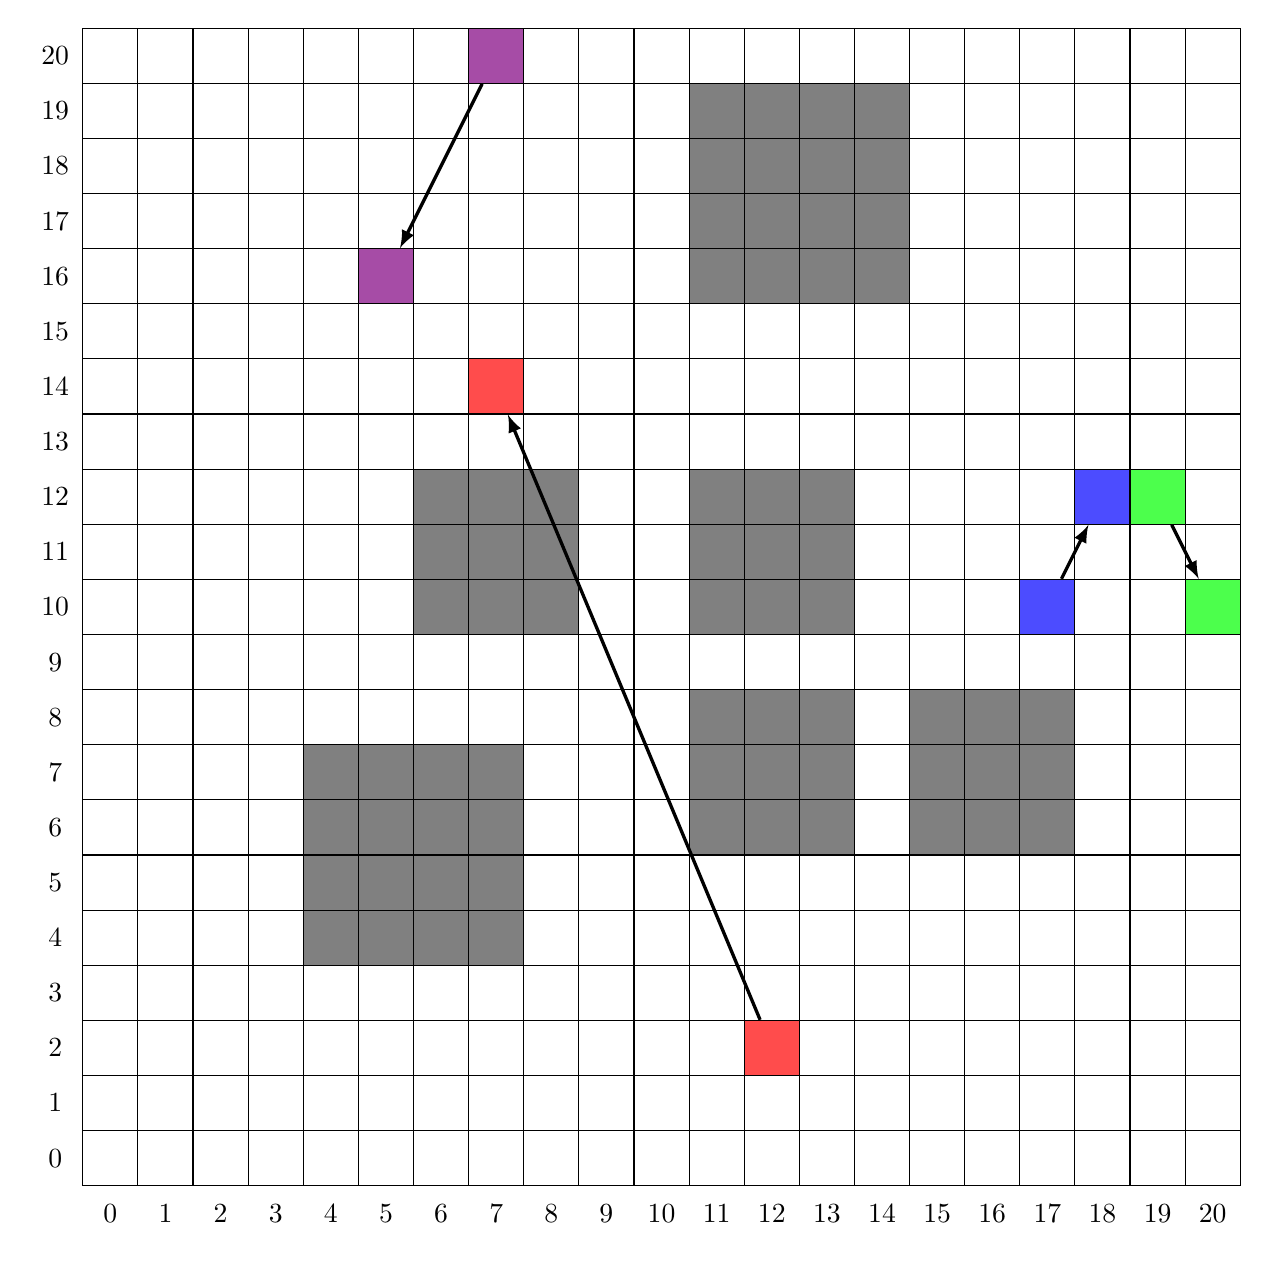
\begin{tikzpicture}[scale=\scale,
	%inner sep=1cm*\scale*\half,
	inner sep=0,
	minimum size=1cm*\scale,
	>=latex,
	pins/.style={rectangle,draw,fill=brown,font=\scriptsize},
	arrow/.style={->,very thick},
	block/.style={gray}]
	% define the row and column number
	\def \N{21}\def \M{21}
	% blockages
	\blockage{4}{4}{7}{7}
	\blockage{11}{16}{14}{19}
	\blockage{6}{10}{8}{12}
	\blockage{15}{6}{17}{8}
	\blockage{11}{6}{13}{8}
	\blockage{11}{10}{13}{12}
	% nets
	\drawtwopin{Dlt34}{5}{16}{B1}{7}{20}{violet!70}
	\drawtwopin{Dlt34}{7}{14}{Dlt26_to_Dlt34}{12}{2}{red!70}
	\drawtwopin{Dlt31_to_Dlt39}{18}{12}{Dlt31}{17}{10}{blue!70}
	\drawtwopin{W}{20}{10}{Dlt31}{19}{12}{green!70}
	\drawgrid{\N}{\M}
	\end{tikzpicture}
	\caption{DAC05\_subproblem\_44}
	\end{figure}
	\clearpage
	\begin{figure}
	\centering
	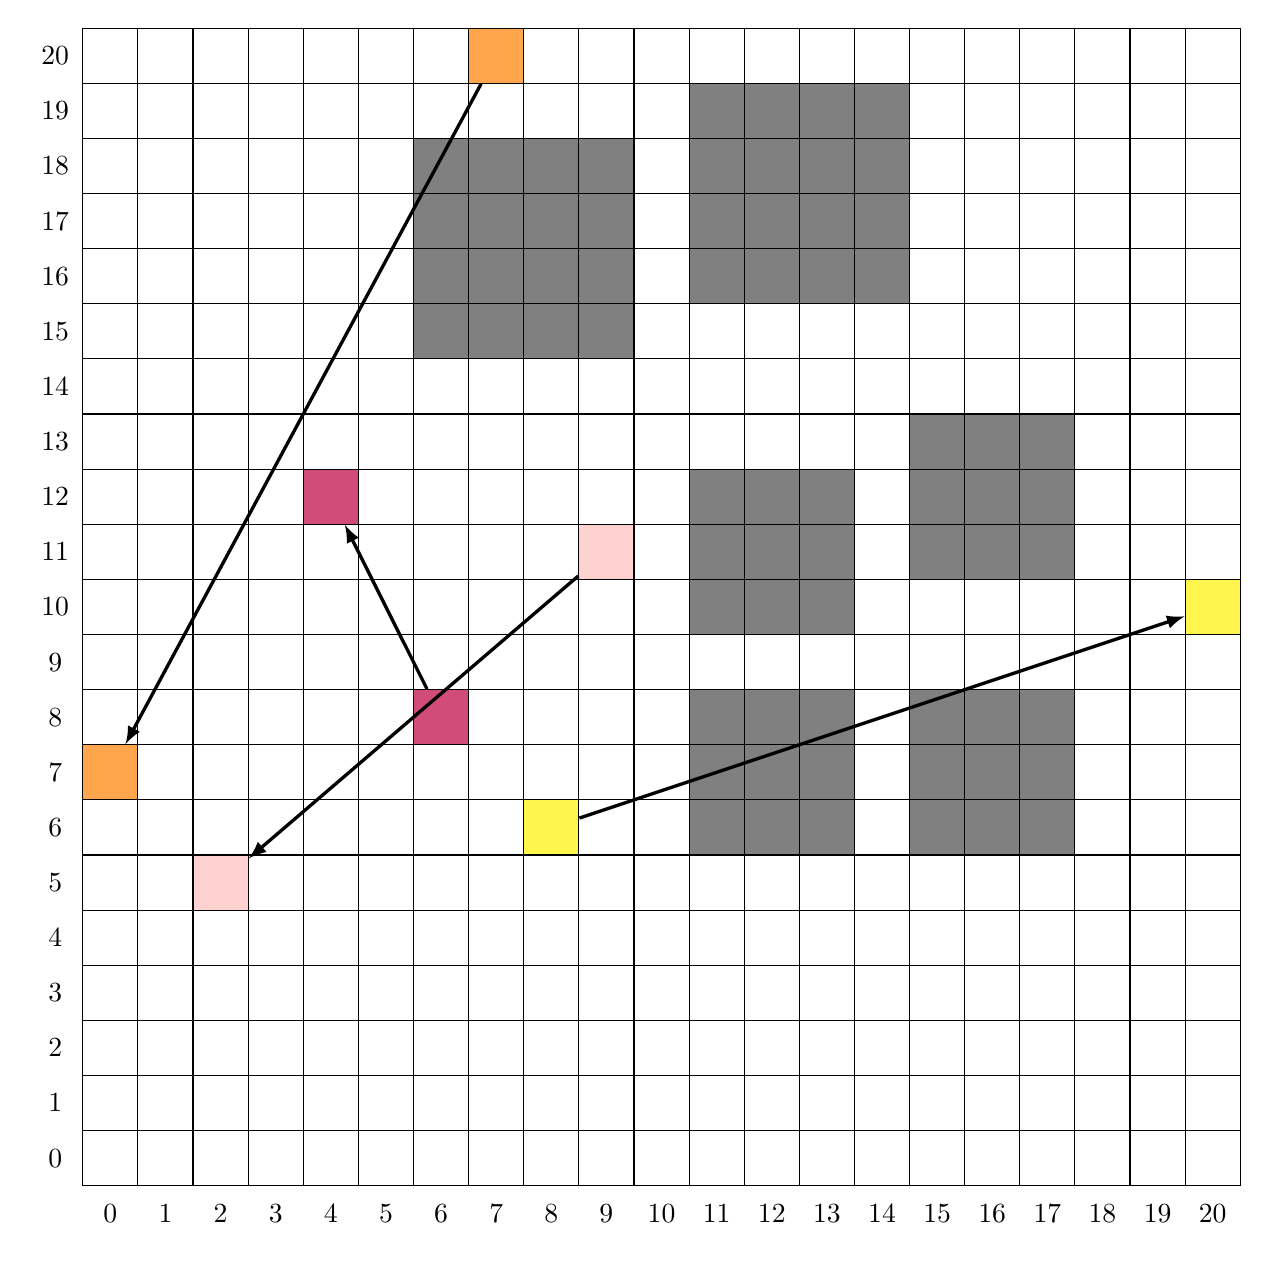
\begin{tikzpicture}[scale=\scale,
	%inner sep=1cm*\scale*\half,
	inner sep=0,
	minimum size=1cm*\scale,
	>=latex,
	pins/.style={rectangle,draw,fill=brown,font=\scriptsize},
	arrow/.style={->,very thick},
	block/.style={gray}]
	% define the row and column number
	\def \N{21}\def \M{21}
	% blockages
	\blockage{11}{16}{14}{19}
	\blockage{6}{15}{9}{18}
	\blockage{15}{6}{17}{8}
	\blockage{11}{6}{13}{8}
	\blockage{11}{10}{13}{12}
	\blockage{15}{11}{17}{13}
	% nets
	\drawtwopin{Dlt35}{0}{7}{B1}{7}{20}{orange!70}
	\drawtwopin{Dlt32_to_Mix01}{4}{12}{Dlt32}{6}{8}{purple!70}
	\drawtwopin{W}{20}{10}{Dlt32}{8}{6}{yellow!70}
	\drawtwopin{Dlt35}{2}{5}{Dlt27_to_Dlt35}{9}{11}{pink!70}
	\drawgrid{\N}{\M}
	\end{tikzpicture}
	\caption{DAC05\_subproblem\_45}
	\end{figure}
	\clearpage
	\begin{figure}
	\centering
	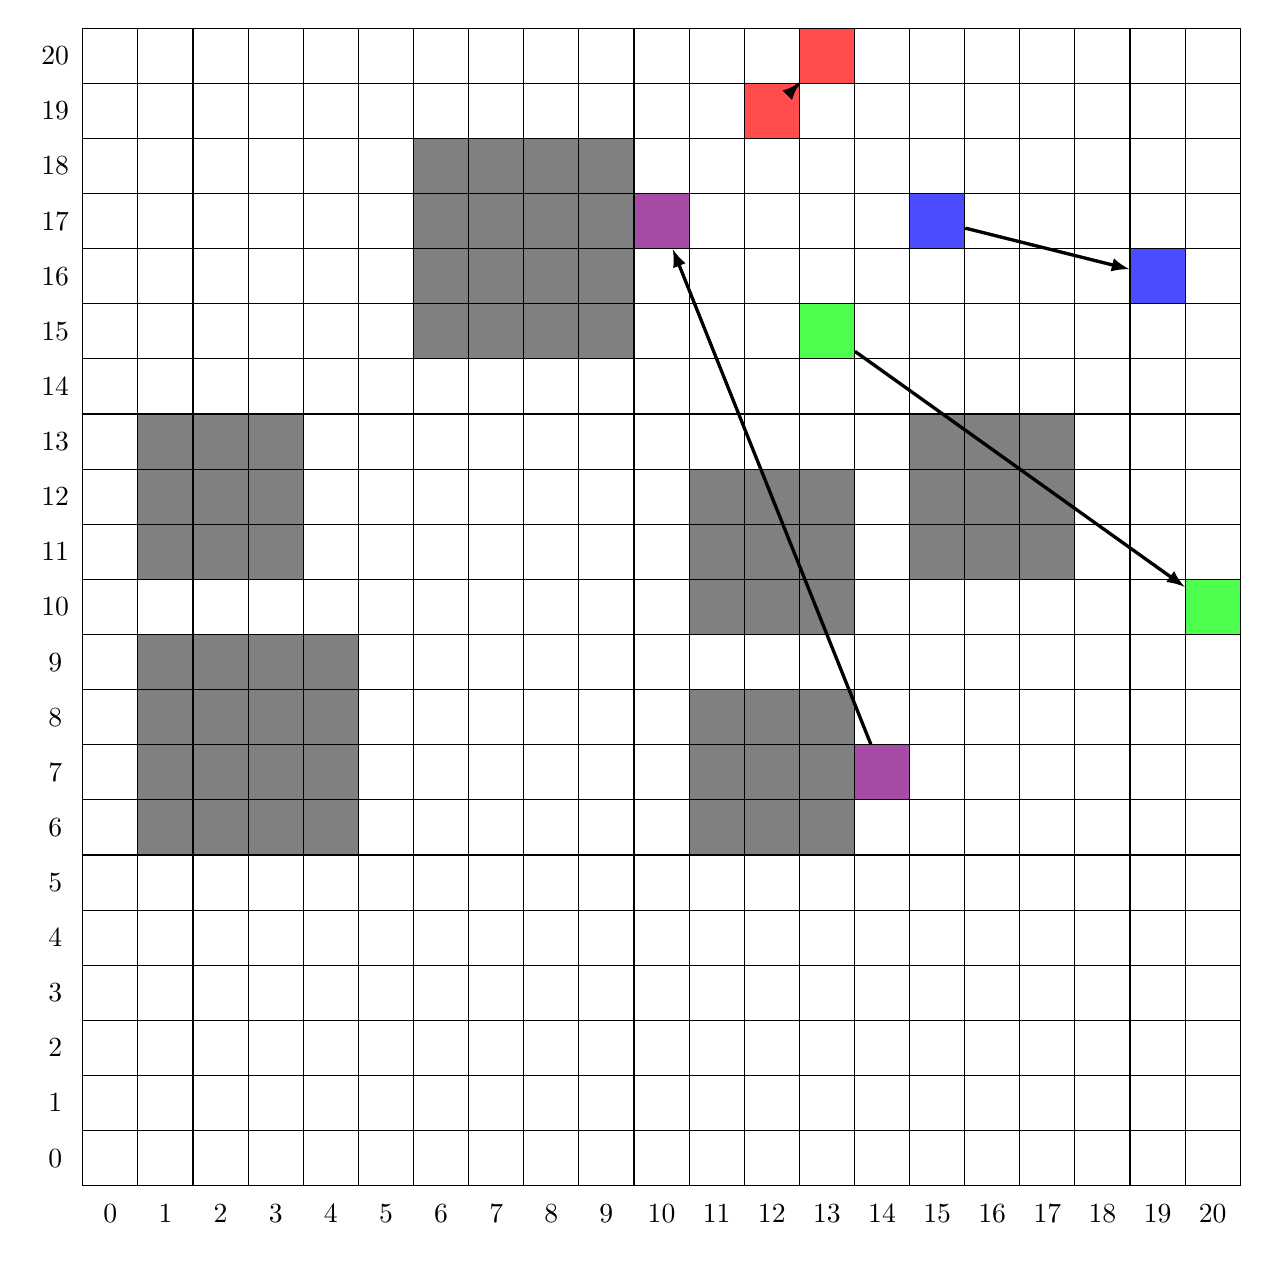
\begin{tikzpicture}[scale=\scale,
	%inner sep=1cm*\scale*\half,
	inner sep=0,
	minimum size=1cm*\scale,
	>=latex,
	pins/.style={rectangle,draw,fill=brown,font=\scriptsize},
	arrow/.style={->,very thick},
	block/.style={gray}]
	% define the row and column number
	\def \N{21}\def \M{21}
	% blockages
	\blockage{6}{15}{9}{18}
	\blockage{1}{6}{4}{9}
	\blockage{11}{6}{13}{8}
	\blockage{11}{10}{13}{12}
	\blockage{15}{11}{17}{13}
	\blockage{1}{11}{3}{13}
	% nets
	\drawtwopin{Dlt36}{10}{17}{Dlt28_to_Dlt36}{14}{7}{violet!70}
	\drawtwopin{Dlt36}{12}{19}{B2}{13}{20}{red!70}
	\drawtwopin{Dlt33_to_Mix02}{19}{16}{Dlt33}{15}{17}{blue!70}
	\drawtwopin{W}{20}{10}{Dlt33}{13}{15}{green!70}
	\drawgrid{\N}{\M}
	\end{tikzpicture}
	\caption{DAC05\_subproblem\_46}
	\end{figure}
	\clearpage
	\begin{figure}
	\centering
	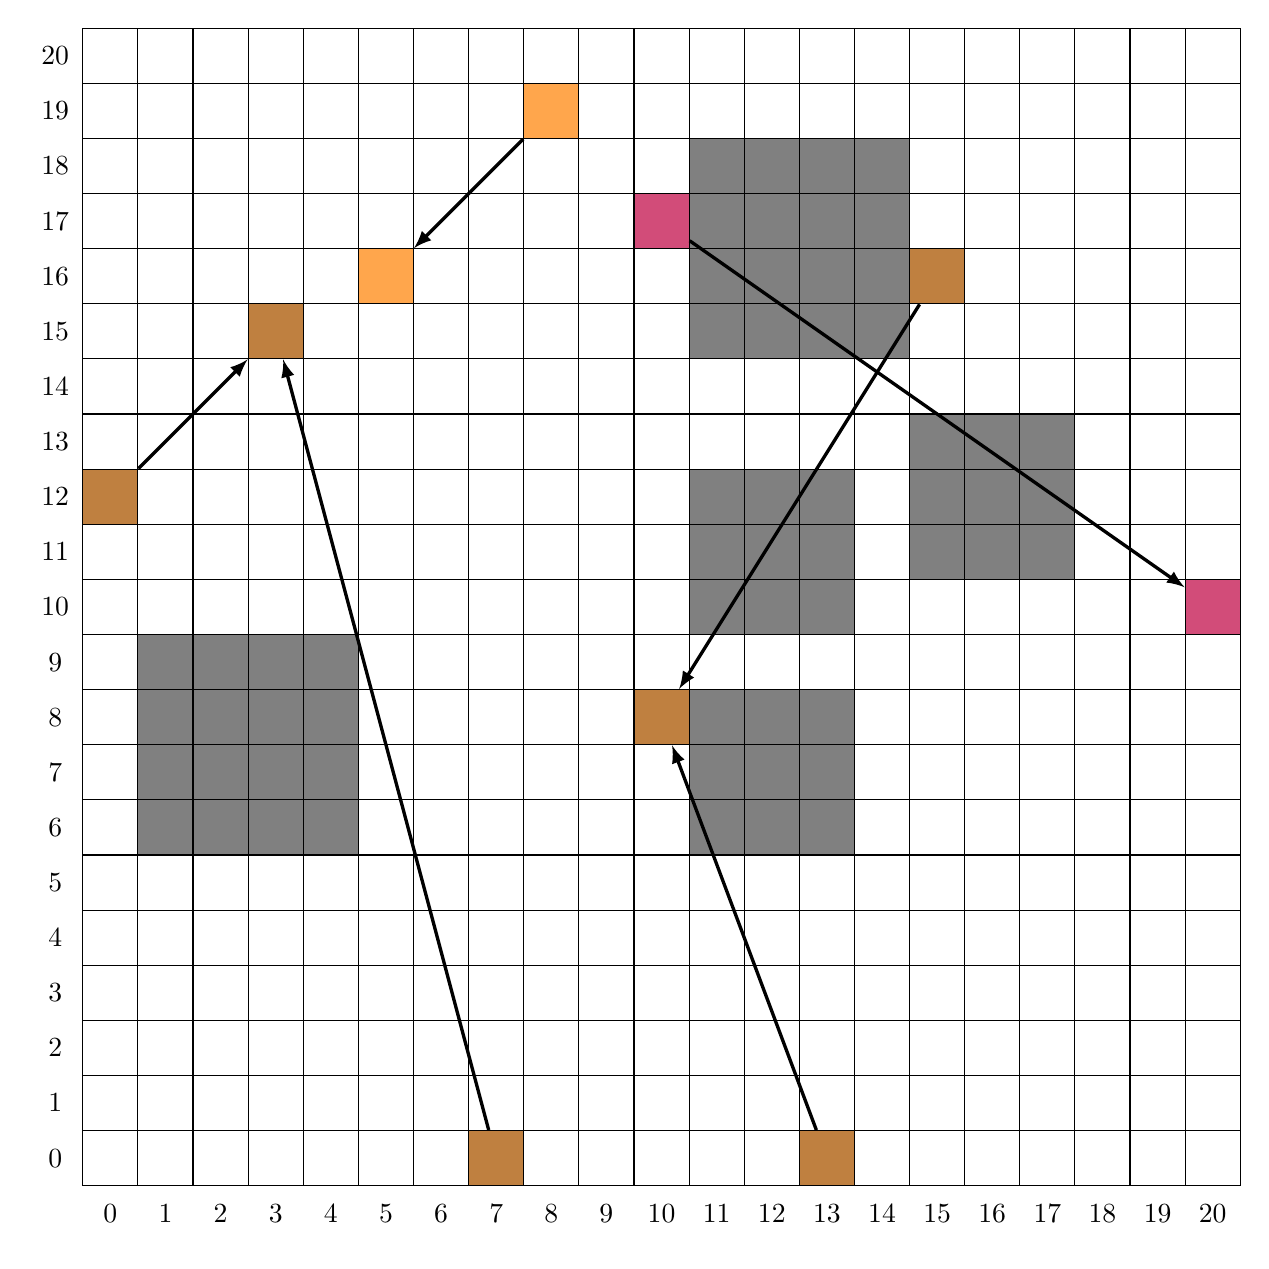
\begin{tikzpicture}[scale=\scale,
	%inner sep=1cm*\scale*\half,
	inner sep=0,
	minimum size=1cm*\scale,
	>=latex,
	pins/.style={rectangle,draw,fill=brown,font=\scriptsize},
	arrow/.style={->,very thick},
	block/.style={gray}]
	% define the row and column number
	\def \N{21}\def \M{21}
	% blockages
	\blockage{1}{6}{4}{9}
	\blockage{11}{15}{14}{18}
	\blockage{11}{6}{13}{8}
	\blockage{11}{10}{13}{12}
	\blockage{15}{11}{17}{13}
	% nets
	\drawthreepin{Mix01}{3}{15}{Dlt32_to_Mix01}{0}{12}{R1}{7}{0}
	\drawthreepin{Mix02}{10}{8}{Dlt33_to_Mix02}{15}{16}{R2}{13}{0}
	\drawtwopin{Dlt34_to_Mix03}{5}{16}{Dlt34}{8}{19}{orange!70}
	\drawtwopin{W}{20}{10}{Dlt34}{10}{17}{purple!70}
	\drawgrid{\N}{\M}
	\end{tikzpicture}
	\caption{DAC05\_subproblem\_47}
	\end{figure}
	\clearpage
	\begin{figure}
	\centering
	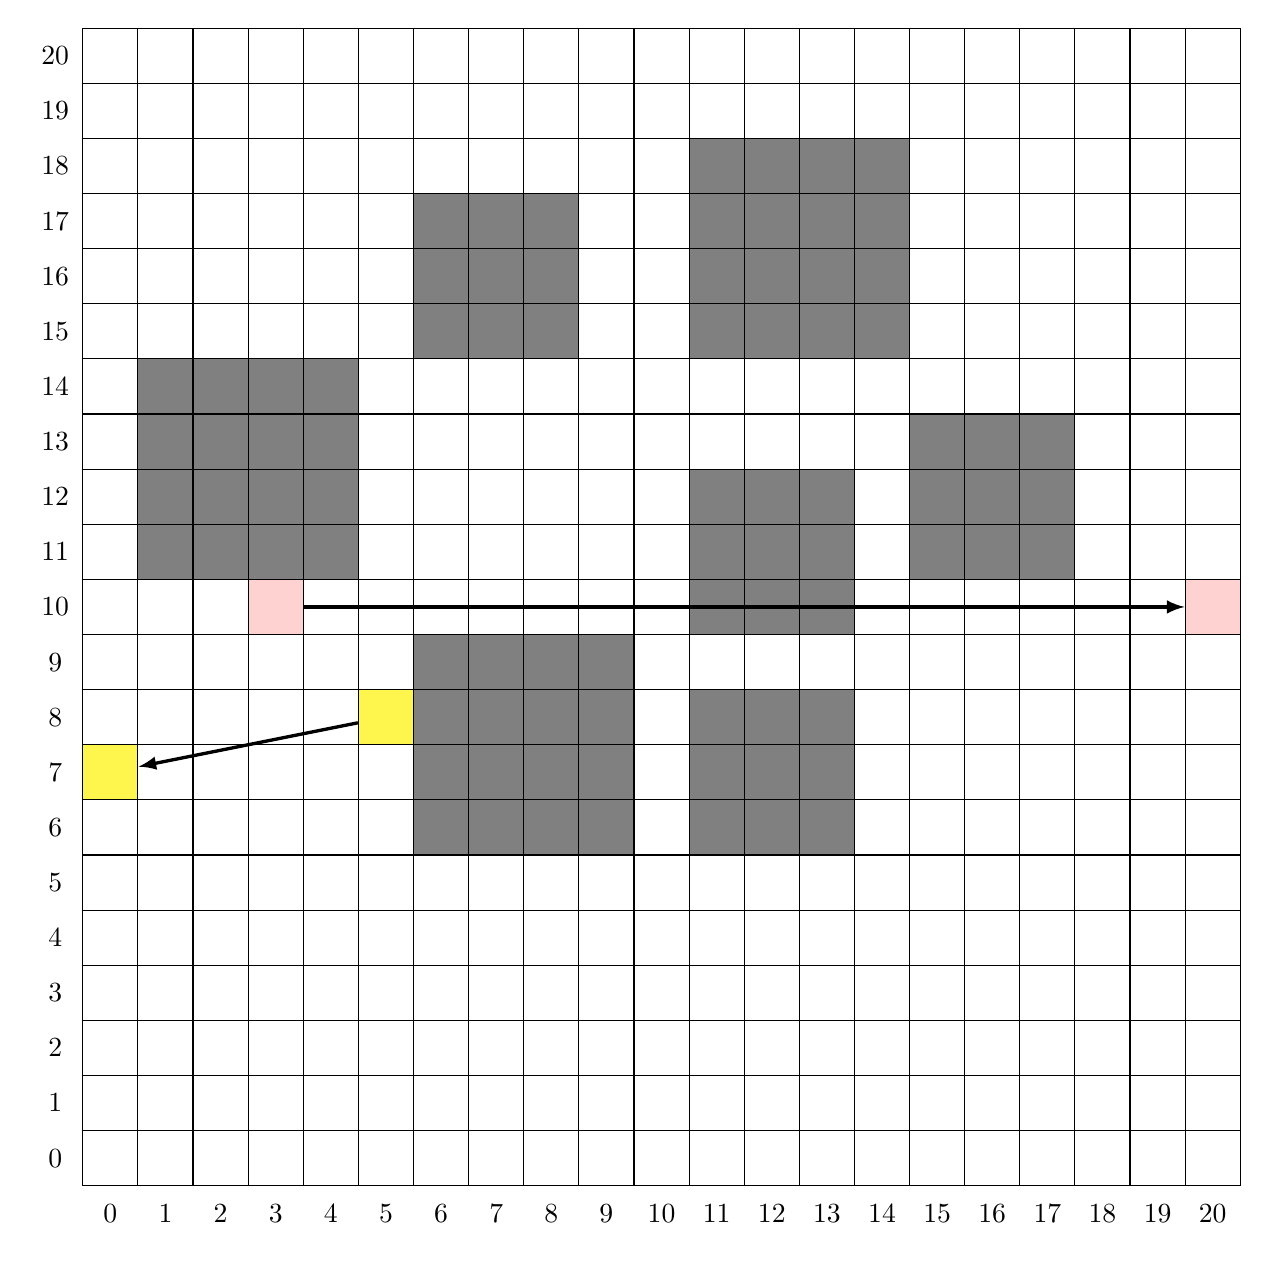
\begin{tikzpicture}[scale=\scale,
	%inner sep=1cm*\scale*\half,
	inner sep=0,
	minimum size=1cm*\scale,
	>=latex,
	pins/.style={rectangle,draw,fill=brown,font=\scriptsize},
	arrow/.style={->,very thick},
	block/.style={gray}]
	% define the row and column number
	\def \N{21}\def \M{21}
	% blockages
	\blockage{11}{15}{14}{18}
	\blockage{1}{11}{4}{14}
	\blockage{6}{6}{9}{9}
	\blockage{11}{6}{13}{8}
	\blockage{11}{10}{13}{12}
	\blockage{15}{11}{17}{13}
	\blockage{6}{15}{8}{17}
	% nets
	\drawtwopin{Dlt35_to_Mix04}{0}{7}{Dlt35}{5}{8}{yellow!70}
	\drawtwopin{W}{20}{10}{Dlt35}{3}{10}{pink!70}
	\drawgrid{\N}{\M}
	\end{tikzpicture}
	\caption{DAC05\_subproblem\_48}
	\end{figure}
	\clearpage
	\begin{figure}
	\centering
	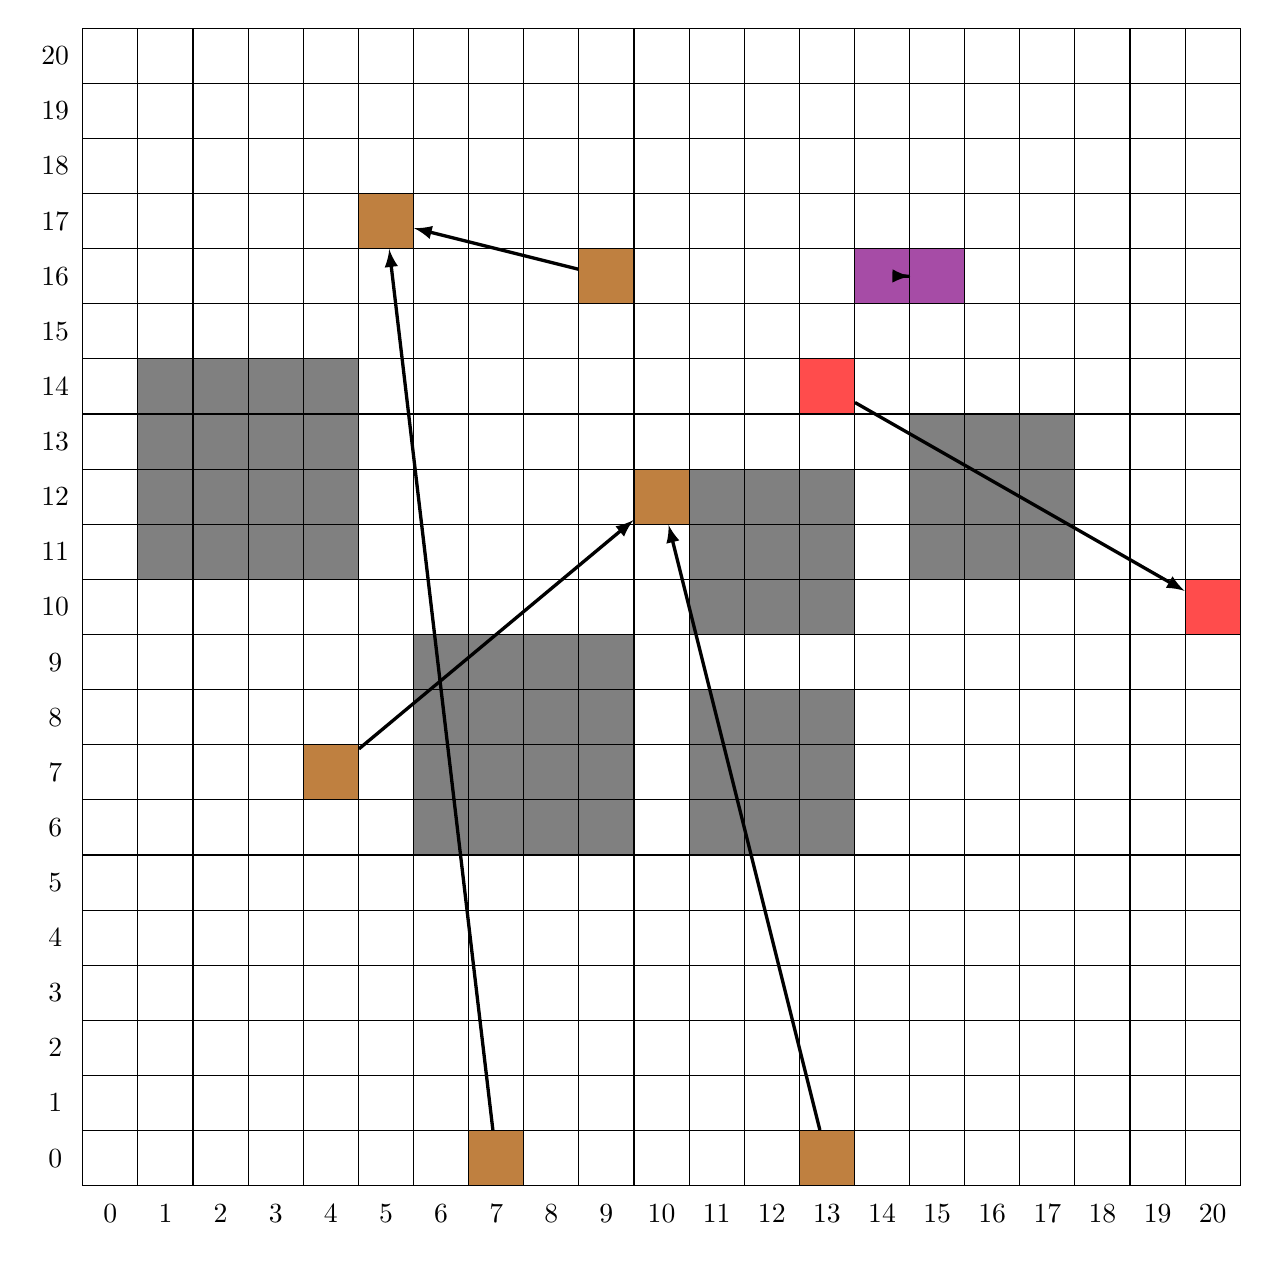
\begin{tikzpicture}[scale=\scale,
	%inner sep=1cm*\scale*\half,
	inner sep=0,
	minimum size=1cm*\scale,
	>=latex,
	pins/.style={rectangle,draw,fill=brown,font=\scriptsize},
	arrow/.style={->,very thick},
	block/.style={gray}]
	% define the row and column number
	\def \N{21}\def \M{21}
	% blockages
	\blockage{1}{11}{4}{14}
	\blockage{6}{6}{9}{9}
	\blockage{11}{6}{13}{8}
	\blockage{11}{10}{13}{12}
	\blockage{15}{11}{17}{13}
	% nets
	\drawtwopin{Dlt36_to_Mix05}{14}{16}{Dlt36}{15}{16}{violet!70}
	\drawtwopin{W}{20}{10}{Dlt36}{13}{14}{red!70}
	\drawthreepin{Mix03}{5}{17}{Dlt34_to_Mix03}{9}{16}{R1}{7}{0}
	\drawthreepin{Mix04}{10}{12}{Dlt35_to_Mix04}{4}{7}{R2}{13}{0}
	\drawgrid{\N}{\M}
	\end{tikzpicture}
	\caption{DAC05\_subproblem\_49}
	\end{figure}
	\clearpage
	\begin{figure}
	\centering
	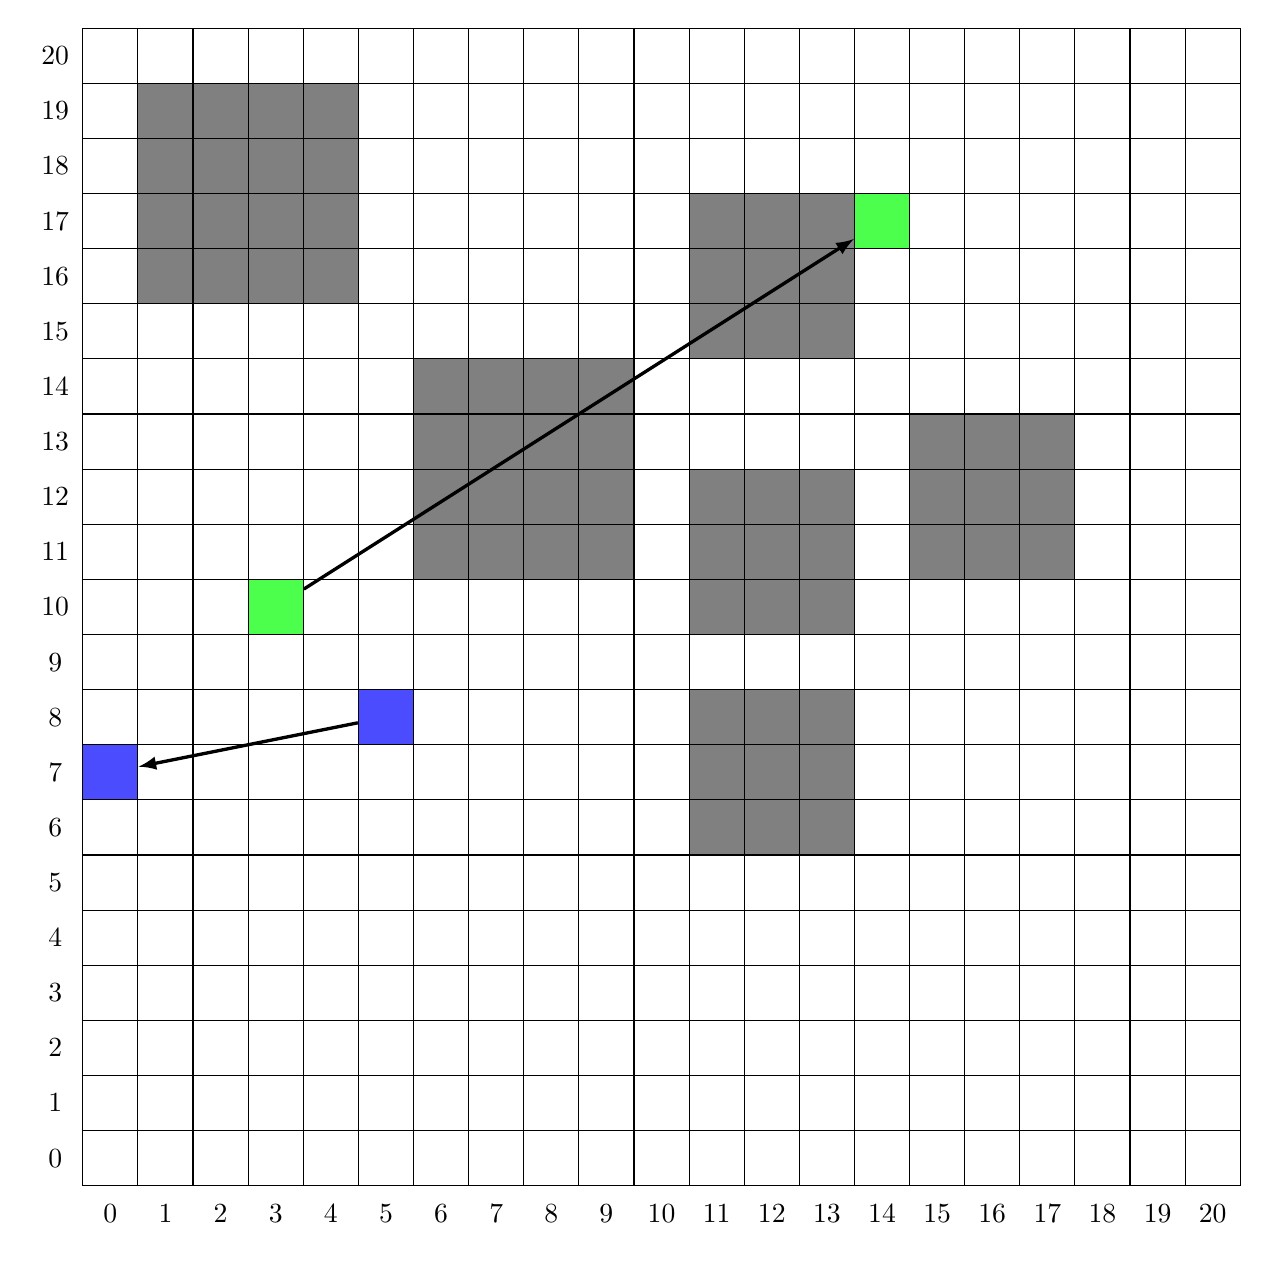
\begin{tikzpicture}[scale=\scale,
	%inner sep=1cm*\scale*\half,
	inner sep=0,
	minimum size=1cm*\scale,
	>=latex,
	pins/.style={rectangle,draw,fill=brown,font=\scriptsize},
	arrow/.style={->,very thick},
	block/.style={gray}]
	% define the row and column number
	\def \N{21}\def \M{21}
	% blockages
	\blockage{1}{16}{4}{19}
	\blockage{6}{11}{9}{14}
	\blockage{11}{6}{13}{8}
	\blockage{11}{10}{13}{12}
	\blockage{15}{11}{17}{13}
	\blockage{11}{15}{13}{17}
	% nets
	\drawtwopin{Opt02}{0}{7}{Mix02}{5}{8}{blue!70}
	\drawtwopin{Opt01}{14}{17}{Mix01}{3}{10}{green!70}
	\drawgrid{\N}{\M}
	\end{tikzpicture}
	\caption{DAC05\_subproblem\_50}
	\end{figure}
	\clearpage
	\begin{figure}
	\centering
	\begin{tikzpicture}[scale=\scale,
	%inner sep=1cm*\scale*\half,
	inner sep=0,
	minimum size=1cm*\scale,
	>=latex,
	pins/.style={rectangle,draw,fill=brown,font=\scriptsize},
	arrow/.style={->,very thick},
	block/.style={gray}]
	% define the row and column number
	\def \N{21}\def \M{21}
	% blockages
	\blockage{1}{16}{4}{19}
	\blockage{6}{11}{9}{14}
	\blockage{15}{16}{17}{18}
	\blockage{1}{6}{3}{8}
	\blockage{15}{11}{17}{13}
	\blockage{11}{15}{13}{17}
	% nets
	\drawtwopin{Dlt37}{4}{8}{Dlt29_to_Dlt37}{14}{7}{orange!70}
	\drawtwopin{Dlt38}{14}{8}{Dlt30_to_Dlt38}{14}{11}{purple!70}
	\drawtwopin{Dlt37}{6}{10}{B1}{7}{20}{yellow!70}
	\drawtwopin{Dlt38}{16}{10}{B2}{13}{20}{pink!70}
	\drawgrid{\N}{\M}
	\end{tikzpicture}
	\caption{DAC05\_subproblem\_51}
	\end{figure}
	\clearpage
	\begin{figure}
	\centering
	\begin{tikzpicture}[scale=\scale,
	%inner sep=1cm*\scale*\half,
	inner sep=0,
	minimum size=1cm*\scale,
	>=latex,
	pins/.style={rectangle,draw,fill=brown,font=\scriptsize},
	arrow/.style={->,very thick},
	block/.style={gray}]
	% define the row and column number
	\def \N{21}\def \M{21}
	% blockages
	\blockage{5}{6}{8}{9}
	\blockage{15}{6}{18}{9}
	\blockage{1}{16}{4}{19}
	\blockage{6}{11}{9}{14}
	\blockage{15}{16}{17}{18}
	\blockage{1}{6}{3}{8}
	\blockage{15}{11}{17}{13}
	% nets
	\drawthreepin{Mix05}{6}{3}{R1}{7}{0}{Dlt36_to_Mix05}{0}{16}
	\drawgrid{\N}{\M}
	\end{tikzpicture}
	\caption{DAC05\_subproblem\_52}
	\end{figure}
	\clearpage
	\begin{figure}
	\centering
	\begin{tikzpicture}[scale=\scale,
	%inner sep=1cm*\scale*\half,
	inner sep=0,
	minimum size=1cm*\scale,
	>=latex,
	pins/.style={rectangle,draw,fill=brown,font=\scriptsize},
	arrow/.style={->,very thick},
	block/.style={gray}]
	% define the row and column number
	\def \N{21}\def \M{21}
	% blockages
	\blockage{5}{6}{8}{9}
	\blockage{15}{6}{18}{9}
	\blockage{2}{1}{5}{4}
	\blockage{15}{16}{17}{18}
	\blockage{1}{6}{3}{8}
	\blockage{15}{11}{17}{13}
	% nets
	\drawtwopin{Opt04}{0}{11}{Mix04}{5}{12}{violet!70}
	\drawtwopin{Opt03}{4}{12}{Mix03}{0}{17}{red!70}
	\drawgrid{\N}{\M}
	\end{tikzpicture}
	\caption{DAC05\_subproblem\_53}
	\end{figure}
	\clearpage
	\begin{figure}
	\centering
	\begin{tikzpicture}[scale=\scale,
	%inner sep=1cm*\scale*\half,
	inner sep=0,
	minimum size=1cm*\scale,
	>=latex,
	pins/.style={rectangle,draw,fill=brown,font=\scriptsize},
	arrow/.style={->,very thick},
	block/.style={gray}]
	% define the row and column number
	\def \N{21}\def \M{21}
	% blockages
	\blockage{5}{6}{8}{9}
	\blockage{15}{6}{18}{9}
	\blockage{2}{1}{5}{4}
	\blockage{15}{16}{17}{18}
	\blockage{1}{6}{3}{8}
	\blockage{5}{11}{7}{13}
	\blockage{1}{10}{3}{12}
	% nets
	\drawtwopin{Dlt39}{11}{5}{B2}{13}{20}{blue!70}
	\drawtwopin{Dlt39}{9}{7}{Dlt31_to_Dlt39}{14}{12}{green!70}
	\drawgrid{\N}{\M}
	\end{tikzpicture}
	\caption{DAC05\_subproblem\_54}
	\end{figure}
	\clearpage
	\begin{figure}
	\centering
	\begin{tikzpicture}[scale=\scale,
	%inner sep=1cm*\scale*\half,
	inner sep=0,
	minimum size=1cm*\scale,
	>=latex,
	pins/.style={rectangle,draw,fill=brown,font=\scriptsize},
	arrow/.style={->,very thick},
	block/.style={gray}]
	% define the row and column number
	\def \N{21}\def \M{21}
	% blockages
	\blockage{10}{6}{13}{9}
	\blockage{15}{16}{17}{18}
	\blockage{1}{6}{3}{8}
	\blockage{5}{11}{7}{13}
	\blockage{1}{10}{3}{12}
	% nets
	\drawtwopin{Mix05_to_Opt05}{0}{16}{Mix05}{1}{3}{orange!70}
	\drawtwopin{Dlt37_to_Mix06}{4}{7}{Dlt37}{7}{10}{purple!70}
	\drawtwopin{W}{20}{10}{Dlt37}{9}{8}{yellow!70}
	\drawtwopin{Dlt38_to_Mix07}{18}{12}{Dlt38}{17}{5}{pink!70}
	\drawtwopin{W}{20}{10}{Dlt38}{19}{7}{violet!70}
	\drawgrid{\N}{\M}
	\end{tikzpicture}
	\caption{DAC05\_subproblem\_55}
	\end{figure}
	\clearpage
	\begin{figure}
	\centering
	\begin{tikzpicture}[scale=\scale,
	%inner sep=1cm*\scale*\half,
	inner sep=0,
	minimum size=1cm*\scale,
	>=latex,
	pins/.style={rectangle,draw,fill=brown,font=\scriptsize},
	arrow/.style={->,very thick},
	block/.style={gray}]
	% define the row and column number
	\def \N{21}\def \M{21}
	% blockages
	\blockage{15}{16}{17}{18}
	\blockage{1}{6}{3}{8}
	\blockage{5}{11}{7}{13}
	\blockage{1}{10}{3}{12}
	\blockage{1}{15}{3}{17}
	% nets
	\drawthreepin{Mix06}{4}{7}{Dlt37_to_Mix06}{8}{7}{R1}{7}{0}
	\drawthreepin{Mix07}{11}{17}{Dlt38_to_Mix07}{14}{12}{R2}{13}{0}
	\drawtwopin{Dlt39_to_Mix08}{13}{7}{Dlt39}{12}{10}{red!70}
	\drawtwopin{W}{20}{10}{Dlt39}{14}{8}{blue!70}
	\drawgrid{\N}{\M}
	\end{tikzpicture}
	\caption{DAC05\_subproblem\_56}
	\end{figure}
	\clearpage
	\begin{figure}
	\centering
	\begin{tikzpicture}[scale=\scale,
	%inner sep=1cm*\scale*\half,
	inner sep=0,
	minimum size=1cm*\scale,
	>=latex,
	pins/.style={rectangle,draw,fill=brown,font=\scriptsize},
	arrow/.style={->,very thick},
	block/.style={gray}]
	% define the row and column number
	\def \N{21}\def \M{21}
	% blockages
	\blockage{5}{6}{8}{9}
	\blockage{7}{16}{10}{19}
	\blockage{15}{16}{17}{18}
	\blockage{1}{6}{3}{8}
	\blockage{5}{11}{7}{13}
	\blockage{1}{10}{3}{12}
	\blockage{1}{15}{3}{17}
	% nets
	\drawthreepin{Mix08}{13}{12}{Dlt39_to_Mix08}{9}{7}{R2}{13}{0}
	\drawgrid{\N}{\M}
	\end{tikzpicture}
	\caption{DAC05\_subproblem\_57}
	\end{figure}
	\clearpage
	\begin{figure}
	\centering
	\begin{tikzpicture}[scale=\scale,
	%inner sep=1cm*\scale*\half,
	inner sep=0,
	minimum size=1cm*\scale,
	>=latex,
	pins/.style={rectangle,draw,fill=brown,font=\scriptsize},
	arrow/.style={->,very thick},
	block/.style={gray}]
	% define the row and column number
	\def \N{21}\def \M{21}
	% blockages
	\blockage{5}{6}{8}{9}
	\blockage{7}{16}{10}{19}
	\blockage{9}{11}{12}{14}
	\blockage{5}{11}{7}{13}
	\blockage{1}{10}{3}{12}
	\blockage{1}{15}{3}{17}
	% nets
	\drawtwopin{W}{20}{10}{Opt01}{18}{17}{green!70}
	\drawtwopin{W}{20}{10}{Opt02}{4}{7}{orange!70}
	\drawgrid{\N}{\M}
	\end{tikzpicture}
	\caption{DAC05\_subproblem\_58}
	\end{figure}
	\clearpage
	\begin{figure}
	\centering
	\begin{tikzpicture}[scale=\scale,
	%inner sep=1cm*\scale*\half,
	inner sep=0,
	minimum size=1cm*\scale,
	>=latex,
	pins/.style={rectangle,draw,fill=brown,font=\scriptsize},
	arrow/.style={->,very thick},
	block/.style={gray}]
	% define the row and column number
	\def \N{21}\def \M{21}
	% blockages
	\blockage{9}{11}{12}{14}
	\blockage{5}{11}{7}{13}
	\blockage{1}{10}{3}{12}
	\blockage{1}{15}{3}{17}
	% nets
	\drawtwopin{Opt06}{0}{7}{Mix06}{9}{7}{purple!70}
	\drawtwopin{Opt07}{14}{17}{Mix07}{6}{17}{yellow!70}
	\drawgrid{\N}{\M}
	\end{tikzpicture}
	\caption{DAC05\_subproblem\_59}
	\end{figure}
	\clearpage
	\begin{figure}
	\centering
	\begin{tikzpicture}[scale=\scale,
	%inner sep=1cm*\scale*\half,
	inner sep=0,
	minimum size=1cm*\scale,
	>=latex,
	pins/.style={rectangle,draw,fill=brown,font=\scriptsize},
	arrow/.style={->,very thick},
	block/.style={gray}]
	% define the row and column number
	\def \N{21}\def \M{21}
	% blockages
	\blockage{9}{11}{12}{14}
	\blockage{1}{6}{3}{8}
	\blockage{15}{16}{17}{18}
	% nets
	\drawtwopin{Opt05}{4}{12}{Mix05_to_Opt05}{4}{16}{pink!70}
	\drawtwopin{W}{20}{10}{Opt03}{8}{12}{violet!70}
	\drawtwopin{W}{20}{10}{Opt04}{4}{11}{red!70}
	\drawgrid{\N}{\M}
	\end{tikzpicture}
	\caption{DAC05\_subproblem\_60}
	\end{figure}
	\clearpage
	\begin{figure}
	\centering
	\begin{tikzpicture}[scale=\scale,
	%inner sep=1cm*\scale*\half,
	inner sep=0,
	minimum size=1cm*\scale,
	>=latex,
	pins/.style={rectangle,draw,fill=brown,font=\scriptsize},
	arrow/.style={->,very thick},
	block/.style={gray}]
	% define the row and column number
	\def \N{21}\def \M{21}
	% blockages
	\blockage{5}{11}{7}{13}
	\blockage{1}{6}{3}{8}
	\blockage{15}{16}{17}{18}
	% nets
	\drawtwopin{Opt08}{0}{11}{Mix08}{8}{12}{blue!70}
	\drawgrid{\N}{\M}
	\end{tikzpicture}
	\caption{DAC05\_subproblem\_61}
	\end{figure}
	\clearpage
	\begin{figure}
	\centering
	\begin{tikzpicture}[scale=\scale,
	%inner sep=1cm*\scale*\half,
	inner sep=0,
	minimum size=1cm*\scale,
	>=latex,
	pins/.style={rectangle,draw,fill=brown,font=\scriptsize},
	arrow/.style={->,very thick},
	block/.style={gray}]
	% define the row and column number
	\def \N{21}\def \M{21}
	% blockages
	\blockage{5}{11}{7}{13}
	\blockage{1}{10}{3}{12}
	% nets
	\drawtwopin{W}{20}{10}{Opt06}{4}{7}{green!70}
	\drawtwopin{W}{20}{10}{Opt07}{18}{17}{orange!70}
	\drawgrid{\N}{\M}
	\end{tikzpicture}
	\caption{DAC05\_subproblem\_62}
	\end{figure}
	\clearpage
	\begin{figure}
	\centering
	\begin{tikzpicture}[scale=\scale,
	%inner sep=1cm*\scale*\half,
	inner sep=0,
	minimum size=1cm*\scale,
	>=latex,
	pins/.style={rectangle,draw,fill=brown,font=\scriptsize},
	arrow/.style={->,very thick},
	block/.style={gray}]
	% define the row and column number
	\def \N{21}\def \M{21}
	% blockages
	\blockage{1}{10}{3}{12}
	% nets
	\drawtwopin{W}{20}{10}{Opt05}{8}{12}{purple!70}
	\drawgrid{\N}{\M}
	\end{tikzpicture}
	\caption{DAC05\_subproblem\_63}
	\end{figure}
	\clearpage
	\begin{figure}
	\centering
	\begin{tikzpicture}[scale=\scale,
	%inner sep=1cm*\scale*\half,
	inner sep=0,
	minimum size=1cm*\scale,
	>=latex,
	pins/.style={rectangle,draw,fill=brown,font=\scriptsize},
	arrow/.style={->,very thick},
	block/.style={gray}]
	% define the row and column number
	\def \N{21}\def \M{21}
	% blockages
	% nets
	\drawtwopin{W}{20}{10}{Opt08}{4}{11}{yellow!70}
	\drawgrid{\N}{\M}
	\end{tikzpicture}
	\caption{DAC05\_subproblem\_64}
	\end{figure}
	\clearpage


\end{document}
